\documentclass[oneside,b5papar,11pt]{book}

\usepackage[protrusion=true,expansion=true]{microtype} % Better typography
\usepackage{graphicx,wrapfig} % Required for including pictures
\usepackage{mathpazo} % Use the Palatino font
\usepackage[T1]{fontenc} % Required for accented characters
\usepackage{amscd,amsmath}
\usepackage{tikz,stmaryrd}
\usepackage{latexsym,amsbsy,bbold, fullpage}
\usepackage{amssymb,amsthm,amsfonts}
\usepackage{pdfsync,yfonts}
\usepackage{tkz-graph,tikz-cd}
\usepackage[all,pdf]{xy}
\usepackage{ctex}
\usepackage{titlesec}
\usepackage{color,xcolor,tcolorbox}
\usepackage{framed}
\usepackage{hyperref,url}
\usepackage{makeidx}
\usepackage[annataritalic]{tengwarscript}%支持Tengwa字母,可以写精灵语了
\usepackage{enumitem}

\def\UrlBreaks{\do\A\do\B\do\C\do\D\do\E\do\F\do\G\do\H\do\I\do\J
\do\K\do\L\do\M\do\N\do\O\do\P\do\Q\do\R\do\S\do\T\do\U\do\V
\do\W\do\X\do\Y\do\Z\do\[\do\\\do\]\do\^\do\_\do\`\do\a\do\b
\do\c\do\d\do\e\do\f\do\g\do\h\do\i\do\j\do\k\do\l\do\m\do\n
\do\o\do\p\do\q\do\r\do\s\do\t\do\u\do\v\do\w\do\x\do\y\do\z
\do\.\do\@\do\\\do\/\do\!\do\_\do\|\do\;\do\>\do\]\do\)\do\,
\do\?\do\'\do+\do\=\do\#}%URL换行咒语

\usetikzlibrary{matrix, calc, arrows}
\usetikzlibrary{patterns,trees,snakes}

\makeindex

%%%%%%%%%%%%%%%%%%%%%%%%%%%%%%%%%%%%%%%%%%%%%%%%%%%%
%在此处调整 定义、定理、性质、引理、公理 的背景颜色%
\newcommand{\chapterbackgroundcolor}{
  \definecolor{shadecolor}{RGB}{255,227,170}
}

\newcommand*{\thmcolor}{185,181,134}
\newcommand*{\propcolor}{201,198,160}
\newcommand*{\lemmacolor}{225,225,200}
\newcommand*{\axiomcolor}{247,247,249}
\newcommand*{\definitioncolor}{173,197,165}
\newcommand*{\notationcolor}{208,222,203}
%%%%%%%%%%%%%%%%%%%%%%%%%%%%%%%%%%%%%%%%%%%%%%%%%%%%

%%%%%%%%%%%%%%%%%%%%%%%%%%%%%%%%%%%%
%%%%%这里调用了曲豆豆的独家秘籍%%%%%
%这是曲豆豆的红包

%%%%%%%%%%%%%%定理环境%%%%%%%%%%%%%%%%%%%%%%%

\newtheorem{mythm}{定理}[section]
\newtheorem{mylemma}[mythm]{引理}
\newtheorem{myprop}[mythm]{性质}
\newtheorem{myaxiom}[mythm]{公理}
\newtheorem{mydefinition}[mythm]{定义}
\newtheorem{mynotation}[mythm]{记号}
\newtheorem{example}[mythm]{例子}
\newtheorem{PreImportantExample}[mythm]{重要例子}
\newtheorem{rem}[mythm]{注记}
\newtheorem{mycor}[mythm]{推论}
\newtheorem{claim}[mythm]{断言}
\newtheorem{prob}{习题}[section]


\chapterbackgroundcolor


\newenvironment{thm}
  {\definecolor{shadecolor}{RGB}{\thmcolor}
    \begin{shaded}\begin{mythm}}
  {\end{mythm}\end{shaded}
  \chapterbackgroundcolor}

\newenvironment{lemma}
  {\definecolor{shadecolor}{RGB}{\lemmacolor}
    \begin{shaded}\begin{mylemma}}
  {\end{mylemma}\end{shaded}
  \chapterbackgroundcolor}

\newenvironment{prop}
  {\definecolor{shadecolor}{RGB}{\propcolor}
    \begin{shaded}\begin{myprop}}
  {\end{myprop}\end{shaded}
  \chapterbackgroundcolor}

\newenvironment{axiom}
  {\definecolor{shadecolor}{RGB}{\axiomcolor}
    \begin{shaded}\begin{myaxiom}}
  {\end{myaxiom}\end{shaded}
  \chapterbackgroundcolor}

\newenvironment{cor}
  {\definecolor{shadecolor}{RGB}{\lemmacolor}
    \begin{shaded}\begin{mycor}}
  {\end{mycor}\end{shaded}
  \chapterbackgroundcolor}

\newenvironment{definition}
  {\definecolor{shadecolor}{RGB}{\definitioncolor}
    \begin{shaded}\begin{mydefinition}}
  {\end{mydefinition}\end{shaded}
  \chapterbackgroundcolor}

\newenvironment{notation}
  {\definecolor{shadecolor}{RGB}{\notationcolor}
    \begin{shaded}\begin{mynotation}}
  {\end{mynotation}\end{shaded}
  \chapterbackgroundcolor}

\newenvironment{Example}
  {\definecolor{shadecolor}{RGB}{\examplecolor}
    \begin{shaded}\begin{PreImportantExample}}
  {\end{PreImportantExample}\end{shaded}
  \chapterbackgroundcolor}

%%%%%%%%%%%%%%%%%%%%%%%%%%%%%%%%%%%%%%%%%%%%%%%%%%%%%%%%%%%%
\newcommand*{\vs}{\vspace{5pt}}
\newcommand*{\vsp}{\vspace{10pt}}
\newcommand*{\vspp}{\vspace{20pt}}
\newcommand*{\kong}{$\,\,\,$}
\newcommand*{\fengexian}{
  \rule[0pt]{14.3cm}{0.01em}
\vs}
%%%%%%%%%%%%%%%%%%%%%%%%%%%%%%%%%%%%%%%%%%%%%%%%%%%%%%%%%%%%
\newcommand*{\Langle}{\left\langle}
\newcommand*{\Rangle}{\right\rangle}
%%%%%%%%%%%%%%%%%%%%%%%%%%%%%%%%%%%%%%%%%%%%%%%%%%%%%%%%%%%%
\newcommand*{\bbA}{\mathbb{A}}
\newcommand*{\bbB}{\mathbb{B}}
\newcommand*{\bbC}{\mathbb{C}}
\newcommand*{\bbD}{\mathbb{D}}
\newcommand*{\bbE}{\mathbb{E}}
\newcommand*{\bbF}{\mathbb{F}}
\newcommand*{\bbG}{\mathbb{G}}
\newcommand*{\bbH}{\mathbb{H}}
\newcommand*{\bbI}{\mathbb{I}}
\newcommand*{\bbJ}{\mathbb{J}}
\newcommand*{\bbK}{\mathbb{K}}
\newcommand*{\bbL}{\mathbb{L}}
\newcommand*{\bbM}{\mathbb{M}}
\newcommand*{\bbN}{\mathbb{N}}
\newcommand*{\bbO}{\mathbb{O}}
\newcommand*{\bbP}{\mathbb{P}}
\newcommand*{\bbQ}{\mathbb{Q}}
\newcommand*{\bbR}{\mathbb{R}}
\newcommand*{\bbS}{\mathbb{S}}
\newcommand*{\bbT}{\mathbb{T}}
\newcommand*{\bbU}{\mathbb{U}}
\newcommand*{\bbV}{\mathbb{V}}
\newcommand*{\bbW}{\mathbb{W}}
\newcommand*{\bbX}{\mathbb{X}}
\newcommand*{\bbY}{\mathbb{Y}}
\newcommand*{\bbZ}{\mathbb{Z}}

\newcommand*{\mcalA}{\mathcal{A}}
\newcommand*{\mcalB}{\mathcal{B}}
\newcommand*{\mcalC}{\mathcal{C}}
\newcommand*{\mcalD}{\mathcal{D}}
\newcommand*{\mcalE}{\mathcal{E}}
\newcommand*{\mcalF}{\mathcal{F}}
\newcommand*{\mcalG}{\mathcal{G}}
\newcommand*{\mcalH}{\mathcal{H}}
\newcommand*{\mcalI}{\mathcal{I}}
\newcommand*{\mcalJ}{\mathcal{J}}
\newcommand*{\mcalK}{\mathcal{K}}
\newcommand*{\mcalL}{\mathcal{L}}
\newcommand*{\mcalM}{\mathcal{M}}
\newcommand*{\mcalN}{\mathcal{N}}
\newcommand*{\mcalO}{\mathcal{O}}
\newcommand*{\mcalP}{\mathcal{P}}
\newcommand*{\mcalQ}{\mathcal{Q}}
\newcommand*{\mcalR}{\mathcal{R}}
\newcommand*{\mcalS}{\mathcal{S}}
\newcommand*{\mcalT}{\mathcal{T}}
\newcommand*{\mcalU}{\mathcal{U}}
\newcommand*{\mcalV}{\mathcal{V}}
\newcommand*{\mcalW}{\mathcal{W}}
\newcommand*{\mcalX}{\mathcal{X}}
\newcommand*{\mcalY}{\mathcal{Y}}
\newcommand*{\mcalZ}{\mathcal{Z}}

\newcommand*{\mfkg}{\mathfrak{g}}    %Lie algebra
\newcommand*{\mfkh}{\mathfrak{h}}
\newcommand*{\mfkm}{\mathfrak{m}}    %maximal ideal
\newcommand*{\mfkp}{\mathfrak{p}}    %prime ideal
\newcommand*{\mfkq}{\mathfrak{q}}

\newcommand*{\mfkgl}{\mathfrak{gl}}
\newcommand*{\mfksl}{\mathfrak{sl}}
\newcommand*{\mfkso}{\mathfrak{so}}
\newcommand*{\mfksp}{\mathfrak{sp}}

\newcommand*{\bfk}{\boldsymbol{k}}
\newcommand*{\bfp}{\boldsymbol{p}}
\newcommand*{\bfq}{\boldsymbol{q}}
\newcommand*{\bfu}{\boldsymbol{u}}
\newcommand*{\bfv}{\boldsymbol{v}}
\newcommand*{\bfw}{\boldsymbol{w}}
\newcommand*{\bfx}{\boldsymbol{x}}
\newcommand*{\bfy}{\boldsymbol{y}}
\newcommand*{\bfz}{\boldsymbol{z}}

\newcommand*{\Ahat}{\hat{A}}
\newcommand*{\Bhat}{\hat{B}}
\newcommand*{\Chat}{\hat{C}}
\newcommand*{\Dhat}{\hat{D}}
\newcommand*{\Ehat}{\hat{E}}
\newcommand*{\Fhat}{\hat{F}}
\newcommand*{\Ghat}{\hat{G}}
\newcommand*{\Hhat}{\hat{H}}

\newcommand*{\zbar}{\overline{z}}            %complex number
\newcommand*{\wbar}{\overline{w}}
\newcommand*{\taubar}{\overline{\tau}}

\newcommand*{\ftil}{\widetilde{f}}
\newcommand*{\gtil}{\widetilde{g}}
\newcommand*{\htil}{\widetilde{h}}
\newcommand*{\itil}{\widetilde{i}}
\newcommand*{\xtil}{\widetilde{x}}
\newcommand*{\ytil}{\widetilde{y}}
\newcommand*{\ztil}{\widetilde{z}}
\newcommand*{\wtil}{\widetilde{w}}

\newcommand*{\Omgtil}{\widetilde{\Omega}}

\newcommand*{\afa}{\alpha}
\newcommand*{\lmd}{\lambda}
\newcommand*{\Lmd}{\Lambda}
\newcommand*{\sgm}{\sigma}
\newcommand*{\Sgm}{\Sigma}
\newcommand*{\gma}{\gamma}
\newcommand*{\Gma}{\Gamma}
\newcommand*{\dta}{\delta}
\newcommand*{\Dta}{\Delta}
\newcommand*{\omg}{\omega}
\newcommand*{\Omg}{\Omega}
\newcommand*{\veps}{\varepsilon}
\newcommand*{\fai}{\varphi}
\newcommand*{\pai}{\varpi}

%%%%%%%%%%%%%%%%%%%%%%%%%%%%%%%%%%%%%%%%%%%%%%%%

\newcommand*{\ra}{\rightarrow}
\newcommand*{\inj}{\hookrightarrow}
\newcommand*{\surj}{\twoheadrightarrow}
\newcommand*{\xra}{\xrightarrow}
\newcommand*{\xla}{\xleftarrow}
\newcommand*{\llra}{\longleftrightarrow}
\newcommand*{\Llra}{\Longleftrightarrow}
\newcommand*{\rlim}{\varinjlim}                 %colimit,余极限,归纳极限,正向极限
\newcommand*{\llim}{\varprojlim}                %limit,极限,投射极限,逆向极限
\newcommand*{\suobing}{\lrcorner\,}             %张量的缩并

\newcommand*{\xybigrow}{\xymatrixrowsep{5pc}}   %交换图排版专用
\newcommand*{\xybigcol}{\xymatrixcolsep{5pc}}   %增大行、列间距
\newcommand*{\tabularbigrow}{\specialrule{0em}{4pt}{4pt}}

\newcommand*{\pz}{\text{---}}                   %破折号
\newcommand*{\yc}{\triangle}                    %余代数的乘法,co-product
\newcommand*{\p}{\partial}                      %偏微分、边缘算子partial
\newcommand*{\td}{\mathrm{d}}                   %微分算子d
\newcommand*{\pbar}{\overline{\partial}}        %Dolbeaut算子partial-bar
\newcommand*{\ten}{\otimes}                     %张量积tensor product
\newcommand*{\bigten}{\bigotimes}
\newcommand*{\op}{^{\text{op}}}
\newcommand*{\downdot}{_{\bullet}}              %下方黑点,用于同调代数中的链复形
\newcommand*{\ddowndot}{_{\bullet\bullet}}
\newcommand*{\updot}{^{\bullet}}
\newcommand*{\wedgeform}{\bigwedge\nolimits^}
\newcommand*{\ssubset}{\subset\!\subset}        %紧包含
\newcommand*{\vkong}{\varnothing}               %空集

%%%%%%%%%%%%%%%%%%%%%%%%%%%%%%%%%%%%%%%%%%%%%%%%
\newcommand*{\lbar}[1]{\overline{#1}}    %比较长的上横线

\newcommand*{\fps}[1]{[\![#1]\!]}        %Formal power series形式幂级数
\newcommand*{\Ls}[1]{(\!(#1)\!)}         %Laurent series     洛朗级数

\newcommand*{\Choose}[2]
  {\left[{
      #1 \atop
      #2
  }\right]}                              %快速输入小型方括号组合数

\newcommand*{\bbar}[1]
  {\overline{#1}}

\newcommand*{\pp}[1]
  {\frac{\partial   }
        {\partial #1}
  }                               %切向量场,一阶偏微分算子

\newcommand*{\pfrac}[2]
  {\frac{\partial #1}
        {\partial #2}
  }                               %一阶偏微分

\newcommand*{\ppfrac}[2]
  {\frac{\partial^2{#1}}
        {\partial{#2}^2}}          %二阶偏微分

\newcommand*{\pmfrac}[3]
  {\frac{\partial^2{#1}}
        {\partial{#2}\partial{#3}}} %二阶混合偏微分

%amsmath 宏包输入矩阵%
%matrix pmatrix bmatrix Bmatrix vmatrix Vmatrix%
%分别为无括号,小括号,中括号,大括号,竖线,双竖线%
%%%%%%%%%%%%%%%%%%%%%%%%%%%%%%%%%%%%%%%%%%%%%%%%
\DeclareMathOperator{\ad}{ad}         %adjoint
\DeclareMathOperator{\Ass}{Ass}       %Associated Prime
\DeclareMathOperator{\Aut}{Aut}       %automorphism
\DeclareMathOperator{\ch}{char}
\DeclareMathOperator{\cl}{cl}         %classical
\DeclareMathOperator{\Coder}{Coder}   %Co-derivation  并不是“码农”的意思
\DeclareMathOperator{\coker}{coker}   %co-kernel      余核
\DeclareMathOperator{\Conf}{Conf}     %Kontsevich公式当中用到了;configuration of points
\DeclareMathOperator{\Crit}{Crit}     %Critical locus
\DeclareMathOperator{\Der}{Der}       %Derivation        导子
\DeclareMathOperator{\Div}{div}       %divergence     散度
\DeclareMathOperator{\DR}{DR}         %De-Rham
\DeclareMathOperator{\End}{End}       %Endomorphism
\DeclareMathOperator{\Ext}{Ext}
\DeclareMathOperator{\ev}{ev}         %evaluation
\DeclareMathOperator{\Free}{Free}
\DeclareMathOperator{\Gal}{Gal}
\DeclareMathOperator{\HC}{HC}         %Hochschild Cyclic (co)homology
\DeclareMathOperator{\HH}{HH}         %Hochschild (co)homology
\DeclareMathOperator{\Hom}{Hom}
\DeclareMathOperator{\id}{id}         %identity
\DeclareMathOperator{\im}{Im}         %Image
\DeclareMathOperator{\Inn}{Inn}       %Inner Derivation  内导子
\DeclareMathOperator{\Inv}{Inv}
\DeclareMathOperator{\Lie}{Lie}
\DeclareMathOperator{\Mor}{Mor}       %Morphism
\DeclareMathOperator{\Obj}{Obj}
\DeclareMathOperator{\Obs}{Obs}       %Observable
\DeclareMathOperator{\per}{per}       %periodic cyclic complex
\DeclareMathOperator{\PV}{PV}         %Polyvector field
\DeclareMathOperator{\Rep}{Rep}
\DeclareMathOperator{\sgn}{sgn}
\DeclareMathOperator{\Sh}{Sh}
\DeclareMathOperator{\Span}{span}
\DeclareMathOperator{\supp}{supp}     %Support 支撑集
\DeclareMathOperator{\Sym}{Sym}       %Symmetry  对称张量积
\DeclareMathOperator{\Tor}{Tor}
\DeclareMathOperator{\Tot}{Tot}       %Total complex of a double-complex
\DeclareMathOperator{\YM}{YM}         %Yang-Mills   杨振宁-米尔斯

%%%%%%%%%%%%%%%%%%%%%%%%%%%%%%%%%%%%%%%%%%%%%%%%
%%%%%%%%%%%%以下是范畴论记号%%%%%%%%%%%%%%%%%%%%
\DeclareMathOperator{\Commu}{\mathsf{Commu}}
\DeclareMathOperator{\alg}{\mathsf{alg}}
\DeclareMathOperator{\Mod}{\mathsf{Mod}}

\newcommand*{\Modcat}[2]
    {\Mod^{#1}_{#2}}
\newcommand*{\Assalgcat}[2]
    {\mathsf{Ass}\!\text{-}\!\alg^{#1}_{#2}}
\newcommand*{\Commualgcat}[2]
    {\Commu\!\text{-}\!\alg^{#1}_{#2}} 
%%%%%%%%%%%%%%%%%%%%%%%%%%%%%%%%%%%%
%%%%%%%%%%%%%%%%%%%%%%%%%%%%%%%%%%%%

\linespread{1.2} % 调整行间距

\makeatletter
%\renewcommand\@biblabel[1]{\textbf{#1.}}
% 将参考文献的方括号 '[1]' 换成 '1.'

\renewcommand{\@listI}{\itemsep=0pt}
% Reduce the space between items in the itemize and enumerate environments and the bibliography

\renewcommand{\maketitle}{
% Customize the title - do not edit title and author name here, see the TITLE block below
\begin{center} % Right align 可以换成 “flushleft”
{\Huge\@title} % Increase the font size of the title

\vspace{50pt} % 标题与作者之间的行间距

{\Large\@author} % 作者姓名
\\\@date % Date

\vspace{20pt} % 作者与摘要之间的行间距
\end{center}
}


%\renewcommand{\abstractname}{摘要}
% Uncomment to change the name of the abstract to something else

\renewcommand{\bibname}{参考文献}
\renewcommand{\contentsname}{目录}
\renewcommand{\proofname}{证明}
\renewcommand{\indexname}{术语索引}

\titleformat{\chapter}
  {\color{blue}
    \huge\bfseries}
  {第\,\thechapter\,章}
{1em}{}

\newcommand{\mchapter}[1]{
  \begin{shaded}
    \chapter{#1}
  \end{shaded}
}



\title{\textbf{复几何}% Title
} % Subtitle

\author{\textsc{曲豆豆\,\,\,码字} % Author
\\{\textit{南七技校福利社\,\,五道口分社}}}

\date{\today\\
第01稿}

%----------------------------------------------------------------------------------------
\begin{document}

\maketitle

\vspp

\begin{figure}[ht]
\centering
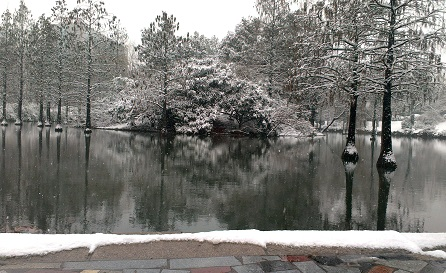
\includegraphics[width=0.7\textwidth]
  {IMAG1546.jpg}

图:中国科学技术大学西校区-也西湖雪景

拍摄于2015.1.28 - 11:30
\end{figure}

本课程参考以下教材:

1. \verb"Demailly: Complex analytic and differential geometry."

2.  \verb"Huybrechts: Complex geometry: an introduction."

3.  \verb"Morrow, Kodaira: Complex manifolds."

4. \verb"Grauert, Remmert: Coherent analytic sheaves."

5. \verb"Hormander: An introduction to complex analysis in several variables."

6. \verb"Griffiths, Harris: Principles of algebraic geometry."

\fengexian

\begin{center}
在五道口也要红专并进、理实交融呀$\sim$
\end{center}

\tableofcontents
\chapter{多复变函数}
%应该补充一些复线性空间的线性代数,单独构成一节。
\section{多元全纯函数}
首先快速回顾单复变函数的知识。
我们通常用$\Omg$来表示$\bbC$的开子集,
$z=x+iy$为$\bbC$的坐标。对于$z\in\bbC$以及实数$R>0$,我们令
$$\bbD(z,R):=\{w\in\bbC|\,|w-z|< R\}$$
为以$z$为圆心$R$为半径的开圆盘。

此外,我们有如下常用记号:
$$\left\{\begin{array}{l}
\td z:=\td x + i\td y\\
\td \bar{z} := \td x- i\td y
\end{array}\right.\quad
\left\{\begin{array}{l}
\pp{z}:=\frac{1}{2}
\left(\pp{x}-i\pp{y}\right)\\
\pp{\bar{z}} := \frac{1}{2}
\left(\pp{x}+i\pp{y}\right)
\end{array}\right.
$$
对于函数$f:\Omg\to\bbC$,
称$f$是\textbf{全纯}(holomorphic)的,
\index{holomorphic function\kong 全纯函数}
若在$\Omg$中成立
$$\pbar f:=\pfrac{f}{\bar{z}}\td\zbar=0$$
我们知道,$f$是全纯的当且仅当$f$在$\Omg$
处处能够局部地展开为收敛幂级数。

对于$\bbC$中的紧致集$K$,称函数$f:K\to\bbC$是全纯的,
如果存在$K$的开邻域$\Omg\supseteq K$,
使得$f$可延拓为$\Omg$上的全纯函数。

单复变函数论中有如下重要结果:

\begin{thm}(柯西积分公式)
设$\bbD\subseteq\bbC$为$\bbC$中的开圆盘,$f:\bbD\to\bbC$为
$\bbD$上的全纯函数,且在$\p\bbD$连续,
则对于任意$w\in\bbD$,成立
$$f(w)=\frac{1}{2\pi i}\int_{\p\bbD}\frac{f(z)}{z-w}\td z$$
\end{thm}

此定理能推导出单变量全纯函数理论的“almost everything”.
这里不再赘述。

我们开始考虑多变量全纯函数。

\begin{definition}
设$\Omg\subseteq\bbC^n$为$\bbC^n$的开子集,函数$f:\Omg\to\bbC$
称为(多变量)\textbf{全纯函数},如果满足以下条件:

(1)$f$是连续函数;

(2)对任意$1\leq j\leq n$,以及任意固定的
$z_1,...,z_{j-1};z_{j+1},...,z_n\in\bbC$,关于$z_j$的单变量函数
$$z_j\mapsto f(z_1,...,z_{j-1};z_j;z_{j+1},...,z_n)$$
是(单变量)全纯函数。
\end{definition}

事实上,如果该定义中的(2)成立,那么能推出(1)成立,
也就是说此定义中的(1)可以去掉。其证明比较复杂,我们承认之。

\begin{notation}
对于$\bbC^n$的开子集$\Omg$,我们记
$$\mcalO(\Omg):=\{f:\Omg\to\bbC|f\text{是$\Omg$上的全纯函数}\}$$
\end{notation}
容易知道$\mcalO(\Omg)$有显然的$\bbC$-代数结构。\vs

本节将说明,多变量全纯函数具有一些与单变量全纯函数类似的性质。

\begin{notation}
对于$z=(z_1,z_2,...,z_n)\in\bbC^n$以及$R=(R_1,R_2,...,R_n)\in\bbR^n$,
并且$R_j>0\,\,(\forall 1\leq j\leq n)$,则我们记
$$\bbD(z,R):=\bbD(z_1,R_1)\times\bbD(z_2,R_2)\times
\cdots\times\bbD(z_n,R_n)$$
称为以$z$为中心,$R$为半径的\textbf{多圆柱}(polydisk)。
\index{polydisk\kong 多圆柱}

对于多圆柱$\bbD(z,R)$,我们记
$$\Gamma(z,R):=\p\bbD(z_1,R_1)\times\p\bbD(z_2,R_2)\times
\cdots\times\p\bbD(z_n,R_n)$$
称为$\bbD(z,R)$的\textbf{特征边界}(distinguished boundary)。
\index{distinguished boundary\kong 特征边界}
\end{notation}
特别注意特征边界$\Gamma(z,R)$
并不等于该多圆柱的边界$\p\bbD(z,R)$.

\begin{thm}(多变量全纯函数的柯西积分公式)

设$f:\overline{\bbD(z,R)}\to\bbC$为全纯函数,
则对任意的$w\in\bbD(z,R)$,成立
$$
  f(w)=
       \frac{1}{(2\pi i)^n}\int_{\Gamma(z,R)}
         \frac{f(\xi)\td\xi_1\td\xi_2\cdots\td\xi_n}
              {(\xi_1-w_1)(\xi_2-w_2)\cdots(\xi_n-w_n)}
$$
\end{thm}
\begin{proof}
由多变量全纯函数的定义,
反复使用单变量全纯函数的柯西积分公式即可。这是容易的。
\end{proof}

与单复变函数完全类似,我们也有泰勒展开:

\begin{cor}(多元全纯函数的泰勒展开公式)

对于$f\in\mcalO(\Omg)$,其中$\Omg\subseteq\bbC^n$为开子集,则
对于任何多圆柱$\bbD(z_0,R)$,如果
$\overline{\bbD(z_0,R)}\subseteq\Omg$,则对于任意$w\in\bbD(z_0,R)$,成立
$$
  f(w)=
       \sum_{\afa\in\bbN^n}a_\afa(w-z_0)^\afa
$$
其中
$$
  a_\afa=\frac{1}{(2\pi i)^n}
           \int_{\Gamma(z_0,R)}
             \frac{f(z)}
                  {(z-z_0)^{\afa+1}}
           \td z_1\td z_2\cdots\td z_n
  =\frac{f^{(\afa)}(z_0)}{\afa!}
$$
\label{多元泰勒-cor}
\end{cor}
注意这里的$\afa$为多重指标,即$\afa=(\afa_1,...,\afa_n)$,
其中每个$\afa_i$都为非负整数。
我们记
\begin{eqnarray*}
z^{\afa}&:=&z_1^{\afa_1}z_2^{\afa_2}\cdots z_n^{\afa_n}\\
\afa!&:=&\afa_1!\afa_2!\cdots\afa_n!\\
f^{(\afa)}&:=&(\p_{z_1})^{\afa_1}(\p_{z_2})^{\afa_2}\cdots(\p_{z_n})^{\afa_n}f\\
\afa+1&:=&(\afa_1+1,\afa_2+1,...,\afa_n+1)
\end{eqnarray*}

其中$z=(z_1,...,z_n)\in\bbC^n$,$f$为$n$元全纯函数。
\begin{proof}
与单复变函数的情形完全类似,可由柯西积分公式得到。
\end{proof}

\begin{thm}(柯西不等式)对于$\bbC^n$的开子集$\Omg$,
若$f\in\mcalO(\Omg)$,多圆柱$\overline{\bbD(z_0,R)}\subseteq\Omg$,
则对任意多重指标$\afa\in\bbN^n$,成立
$$\left|f^{(\afa)}(z_0)\right|\leq
\frac{\afa!}{R^\afa}
\sup_{z\in\Gamma(z_0,R)}|f(z)|$$
\end{thm}
\begin{proof}
与单复变函数的情形完全类似。
利用多元泰勒展开(推论\ref{多元泰勒-cor})即可。
\end{proof}

\begin{cor}设$\Omg\subseteq \bbC^n$为\textbf{连通}开集,
$f\in\mcalO(\Omg)$满足$\forall 1\leq k\leq n$,
$\pfrac{f}{z_k}$在$\Omg$上恒为$0$,则$f$在$\Omg$上为常值函数。
\end{cor}

\begin{cor}(刘维尔定理)
设$f\in\mcalO(\bbC^n)$,并且满足
$$|f(z)|\leq A(1+|z|)^B$$
其中$A,B$为正实数,那么$f$必为次数不超过$B$的多项式函数。
\end{cor}

这些性质于单变量全纯函数雷同,证明也是类似的。

\begin{cor}(Montel定理)

设$\Omg$为$\bbC^n$的开子集,则$\mcalO(\Omg)$
中的任何局部一致有界的全纯函数列都存在一致收敛的子列。
\end{cor}
\begin{proof}
仍类似于单复变全纯函数的情形。使用柯西积分公式,再配合
Arzela-Ascoli定理即可。从略。
\end{proof}

现在,简单介绍一些复的微分形式。对于$\bbC^n$,记其复坐标为
$(z_1,z_2,...,z_n)$;视$\bbC^n$为$2n$维实线性空间,
$$z_k=x_k+iy_k$$
从而引入
\begin{eqnarray*}
\td z_k&=&\td x_k+i\td y_k\qquad (1,0)\text{形式}\\
\td \zbar_k&=&\td x_k-i\td y_k\qquad (0,1)\text{形式}
\end{eqnarray*}

\begin{definition}($(p,q)$-形式)

设$\Omg$为$\bbC^n$的非空开集,则形如
$$u(z)=\sum_{|I|=p\atop |J|=q}
a_{IJ}(z)\td z_I\wedge\td\zbar_J$$
的光滑张量场称为$(p,q)$-形式。
记$\Omg$上的$(p,q)$-形式之全体为$C^\infty_{p,q}(\Omg)$.
\end{definition}
这里的$I,J$为多重指标。“光滑”指的是系数函数$a_{IJ}$为$\Omg$上的光滑复值函数。
另外,显然$(0,0)$-形式即为光滑函数;
$C^\infty_{p,q}(\Omg)$具有显然的复线性空间结构,
事实上还是$C^\infty(\Omg)$-模。

\begin{notation}($\pbar$-算子)
定义算子
$$\pbar: C^\infty_{p,q}(\Omg)\to C^\infty_{p,q+1}(\Omg)$$
如下:对于$(p,q)$-形式
$$u:=\sum_{|I|=p\atop|J|=q}
a_{IJ}\td z_I\wedge\td\zbar_J$$
则
$$
  \pbar u=
  \sum_{|I|=p\atop|J|=q}
    \sum_{k=1}^n
      \pfrac{a_{IJ}}{\zbar_k}
      \td \zbar_k\wedge\td z_I\wedge\td\zbar_J
$$
\end{notation}
类似地,也有
$$\p:C_{p,q}^\infty(\Omg)\to C_{p+1,q}^\infty(\Omg)$$
它们与外微分算子$\td$满足关系
$$\td=\p+\pbar$$
由$\td^2=0$,易知
$$\p^2=0,\quad \pbar^2=0,\quad \p\pbar+\pbar\p=0$$

以下事实显然成立:
\begin{lemma}
对于区域$\Omg$上的光滑函数$f\in C^\infty(\Omg)$,
则$f$全纯当且仅当$\pbar f=0$.
\end{lemma}

\begin{rem}(Dolbeault上同调)
对于$\Omg\subseteq\bbC^n$,注意$\pbar^2=0$,
从而对任意$p\geq 0$,有上链复形$C^\infty_{p,\bullet}(\Omg)$:
$$
  \cdots\to
  C^\infty_{p,q-1}(\Omg)
  \xra{\pbar}C^\infty_{p,q}(\Omg)
  \xra{\pbar}C^\infty_{p,q+1}(\Omg)
  \to\cdots
$$
称上同调群
$$H^{p,q}(\Omg):=H^q(C^\infty_{p,\bullet}(\Omg),\pbar)$$
为区域$\Omg$的\textbf{Dolbeault上同调群}。
\index{Dolbeault cohomology}
\end{rem}
类似于外微分$\td$的de-Rham上同调群,
Dolbeault上同调群与$\Omg$的拓扑联系密切。
例如,以下定理十分重要,我们先陈述,以后再证明:

\begin{lemma}(Dolbeault-Grothendieck引理)

设$\bbD\subseteq\bbC^n$为多圆柱,则对于任意$p,q\geq 0$,
$$H^{p,q}(\bbD)=0$$
\end{lemma}

不难发现它与de Rham上同调的Poincare引理有些类似。

\section{解析延拓与Hartogs现象}
上一节介绍了多复变函数的一些“普通的”(与单变量类似)性质,
本节开始介绍多复变函数的一些独特性质。

\begin{lemma}设$f\in C^\infty_c(\bbC)$为复平面上的
紧支光滑函数,则对任意$z\in\bbC$,成立
$$
  \frac{1}{2\pi i}
  \iint_\bbC
    \frac{\p f\big/\p\taubar}
         {\tau-z}
    \td\tau\wedge\td\taubar
=f(z)$$
\end{lemma}
\begin{proof}
基本的微积分练习。考虑换元$\tau=z+re^{i\theta}$,则易知
\begin{eqnarray*}
  \td\tau\wedge\td\taubar&=&-2ir\td r\wedge\td\theta\\
  \pfrac{r}{\taubar}&=&\frac{1}{2}e^{i\theta}\\
  \pfrac{\theta}{\taubar}&=&-\frac{1}{2ir}e^{i\theta}
\end{eqnarray*}
因此有
\begin{eqnarray*}
     \frac{1}{2\pi i}
     \iint_\bbC
       \frac{\p f\big/\p\taubar}
            {\tau-z}
       \td\tau\wedge\td\taubar
&=&
     \frac{-1}{2\pi}
       \int_0^\infty\td r
         \int_0^{2\pi}
           \left(
            -\frac{1}{ir}\pfrac{f}{\theta}(z+re^{i\theta})
           \right)
           \td\theta\\
& &
    +\frac{-1}{2\pi}
     \int_0^{2\pi}\td\theta
       \int_0^\infty
       \left(
         \pfrac{f}{r}(z+re^{i\theta})
       \right)
       \td r\\
&=&
     0+\frac{-1}{2\pi}
     \int_0^{2\pi}
       -f(z)
       \td\theta\\
&=&
     f(z)
\end{eqnarray*}
证毕。
\end{proof}

\begin{lemma}(简单版本的$\pbar$-引理)

设$n\geq 2$,$\fai\in C^\infty_{0,1}(\bbC^n)$
为具有紧支集的光滑$(0,1)$-形式,
且$\pbar\fai=0$,则存在$\bbC^n$上的紧支光滑函数$g$,使得
$$\pbar g=\fai$$
\label{partial-bar引理-简单版本-lemma}
\end{lemma}

\begin{proof}
记光滑$(0,1)$-形式$\fai$为
$$\fai=\sum_{k=1}^n\fai_k(z_1,...,z_n)\td\zbar_k$$
则
\begin{eqnarray*}
     \pbar\fai
&=&
     \sum_{k,l}
       \pfrac{\fai_k}{\zbar_l}
       \td\zbar_l\wedge\td\zbar_k
 =
     \sum_{1\leq l<k\leq n}
       \left(
         \pfrac{\fai_k}{\zbar_l}
        -\pfrac{\fai_l}{\zbar_k}
       \right)
       \td\zbar_l\wedge\td\zbar_k
\end{eqnarray*}
从而由$\pbar\fai=0$可得对任意$k\neq l$,
$$\pfrac{\fai_k}{\zbar_l}=\pfrac{\fai_l}{\zbar_k}$$

考虑如下的$\bbC^n$上的函数$\psi$:对于$z=(z_1,...,z_n)\in\bbC^n$,
$$
  \psi(z)
:=
  \frac{1}{2\pi i}
  \iint_\bbC
    \frac{\fai_1(\tau;z_2,...,z_n)}
         {\tau-z_1}
    \td\tau\wedge\td\taubar
$$
由$\fai_1$的紧支性易知$\psi$为$\bbC^n$上的光滑函数。
对于$1<k\leq n$,有
\begin{eqnarray*}
     \pfrac{\psi(z)}{\zbar_k}
&=&
     \frac{1}{2\pi i}
     \iint_\bbC
       \frac{\pfrac{\fai_1}{\zbar_k}(\tau;z_2,...,z_n)}
            {\tau-z_1}
       \td\tau\wedge\td\taubar\\
&=&
     \frac{1}{2\pi i}
     \iint_\bbC
       \frac{\pfrac{\fai_k}{\taubar}(\tau;z_2,...,z_n)}
            {\tau-z_1}
       \td\tau\wedge\td\taubar\\
&=&
    \fai_k(z)
\end{eqnarray*}
上式对$k=1$显然也成立。因此$\pbar\psi=\fai$.

最后还需要证明$\psi$是紧支的。
由于$\fai$紧支,存在足够大的$R>0$,使得
$$\supp\fai\subseteq \bbD(0,R)$$
因此任意取定$z\in\bbC^n$,使得$z$的分量$z_2,z_3,...,z_n$之中
至少有一个模长大于$R$,则由$\psi$的定义式直接得到$\psi(z)=0$.
(注意:这一步严重依赖$n\geq 2$!)也就是说,存在$z\not\in\bbD(0,R)$
使得$\psi=0$在$z$的某邻域内都成立。
另一方面,由于$\pbar\psi=\fai$且$\supp\fai\subseteq\bbD(0,R)$,
从而$\psi$在$\bbD(0,\bbR)$外部全纯,因此由解析延拓唯一性,
$\psi$在$\bbD(0,R)$外部恒为零,因此$\psi$紧支。
\end{proof}

此引理在单复变$n=1$的情形\textbf{不成立}:
\begin{example}
设$\fai_1\in C_0^\infty(\bbC)$为复平面上的紧支光滑函数,并且
$$\iint_\bbC\fai_1(z)\neq 0$$
考虑$\bbC$上的$(0,1)$-形式$\fai=\fai_1(z)\td\zbar$,
则$\pbar\fai=0$是平凡的,
但\textbf{不存在}紧支光滑函数$\psi$使得$\pbar\psi=\fai$.
\end{example}

\begin{proof}
若存在紧支光滑函数$\psi$使得$\pbar\psi=\fai$,
则$\pfrac{\psi}{\zbar}=\fai_1$.于是
$$
  0\neq
  \iint_\bbC
    \fai_1(z)\td z\wedge\td\zbar
=
  \iint_\bbC
    \pfrac{\psi}{\zbar}
    \td z\wedge\td\zbar
=0
$$
产生矛盾。
\end{proof}

以下是多复变函数解析延拓的令人惊讶的性质,
它与单复变函数有本质不同:

\begin{thm}(Hartogs现象)

设$\Omg\subseteq\bbC^n$为开集$(n\geq 2)$,
$K\ssubset\Omg$且为$\bbC^n$的紧子集,
则对任意的$f\in\mcalO(\Omg\setminus K)$,
都存在解析延拓$F\in\mcalO(\Omg)$,使得
$$F|_{\Omg\setminus K}=f$$
\end{thm}

\begin{proof}
取$K$与$\Omg$直接的截断函数$\psi\in C^\infty_0(\bbC^n)$,
使得$0\leq \psi\leq 1$,
$$K\ssubset\supp\psi\ssubset\Omg$$
并且$\psi|_K\equiv 1$.
考虑$$\ftil:=(1-\psi)f$$
则$\ftil$在整个$\Omg$上都有定义。注意
$$\pbar\ftil=-(\pbar\psi)f+(1-\psi)\pbar f$$
易知$\supp\pbar\ftil\subseteq\supp\psi$.于是由
引理\ref{partial-bar引理-简单版本-lemma},存在光滑函数
$v$,使得$\supp v\subseteq\psi$,并且$\pbar v=\pbar\ftil$,
从而考虑函数
$$F:=(1-\psi)f-v$$
则$\pbar F=0$,从而$F\in\mcalO(\Omg)$.又因为易知
$$F=f\quad(\forall z\in\Omg\setminus\supp\psi)$$
从而由解析延拓唯一性,有$F_{\Omg\setminus K}=f$.
\end{proof}

关于解析延拓,再介绍如下结果:

\begin{lemma}(Hartogs figure)
\index{Hartogs figure}

对于$n>1$,正实数$0\leq r<R$,
以及$\bbC^{n-1}$的开子集$\omg'\subseteq\omg$,
其中$\omg$是连通的。记$\bbC^n$的开子集
$$
  \Omg:=
    \left(
      (\bbD(0,R)\setminus\bbD(0,r))\times\omg
    \right)
    \cup
    \left(
      \bbD(0,R)\times\omg'
    \right)
$$
其中$\bbD(0,r)$与$\bbD(0,R)$
分别为$\bbC$上的以原点为中心,$r,R$为半径的开圆盘。
则任意$f\in\mcalO(\Omg)$都可以(唯一地)解析延拓至
$$\widetilde{\Omg}:=\bbD(0,R)\times\omg$$
\end{lemma}
如此的区域$\Omg$称之为“\textbf{Hartogs figure}”。
$\Omg$的几何图像大致如下:

\begin{figure}[ht]
\centering
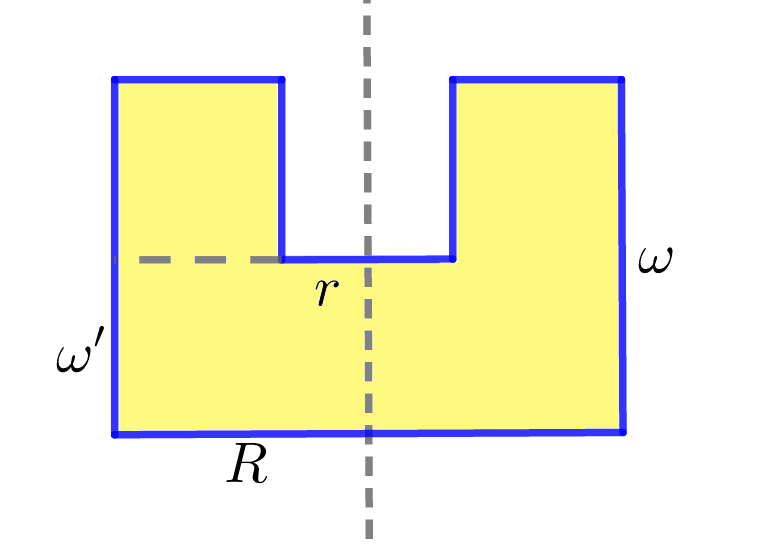
\includegraphics[width=0.4\textwidth]
  {figures/HartogsFigure.png}

图:Hartogs figure示意
\end{figure}

\begin{proof}
容易知道
$$\Omg=\big\{(z_1,\ztil)\in\bbC\times\bbC^{n-1}\big|
r<|z_1|<R,\ztil\in\omg\text{或者}
|z_1|\leq r,\ztil\in\omg'
\big\}$$
对于$f\in\mcalO(\Omg)$,定义$\Omgtil$上的函数
$$
  \ftil(z_1,\ztil):=
    \frac{1}{2\pi i}
    \int_{|w|=\rho}
      \frac{f(w,\ztil)}
           {z_1-w}
      \td w
$$
其中$\rho$为满足$\max\{r,|z_1|\}<\rho<R$的任意实数。
则易知如此定义的$\ftil$为$f$在$\Omgtil$上的解析延拓。
\end{proof}

\begin{thm}(Riemann延拓定理)

考虑$\bbC^n$中的多圆柱$\bbD(0,R)$,其中$n\geq 2$,$R\in\bbR_+^n$。
对任意$2\leq p\leq n$,令$\bbC^n$的子集
$$S:={(z_1,...,z_n)\in\bbC^n|z_1=\cdots=z_p=0}$$
则对任意$f\in\mcalO(\bbD(0,R)\setminus S)$,
$f$都可(唯一地)解析延拓至$\bbD(0,R)$.
\end{thm}

\begin{proof}
这是Hartogs figure的显然推论。记$R=(R_1,R_2,...,R_n)$,
以及$R':=(R_2,...,R_n)\in\bbR^{n-1}$.
考虑$\bbC^{n-1}$的开子集
\begin{eqnarray*}
  \omg &:=&\bbD(0,R')\\
  \omg'&:=&\omg\setminus\{z_2=\cdots=z_p=0\}
\end{eqnarray*}
则易知
$$\bbD(0,R)\setminus S=
\Big(
  \bbD(0,R_1)\setminus\{0\}\times\omg
\Big)
\cup
\Big(
  \bbD(0,R_1)\times\omg'
\Big)
$$
为Hartogs figure,从而完。
\end{proof}

\section{Weierstrass预备定理与除法定理}
(待补)







%%%%%%%%%%%%%%%%%%%%%%%%%%%%%%%%%%%%%%%%%%%%%%%%%
%%%%%%%%%%%%%%%%%%%%%%%%%%%%%%%%%%%%%%%%%%%%%%%%%
%       2019.3.21启用电子稿                     %
%%%%%%%%%%%%%%%%%%%%%%%%%%%%%%%%%%%%%%%%%%%%%%%%%

\chapter{层与层上同调}
\section{层的上同调}
Today:

Sheaf cohomology

$X$ a topological space, $\mcalF$- sheaf (of abelian groups).

\begin{definition}  (resolution)

(1)a resolution of $\mcalF$ is an exact sequence

$$0\to \mcalF\xra{j}\mcalF\xra{d^0}\mcalF\xra{d^1}\to\cdots$$

\end{definition}

\begin{definition}
A sheaf $\mcalA$ is called injective, if
if for any injective morphism $j:\mcalA\to \mcalB$
and for any morphism $\fai:\mcalA\to\mcalS$,
there exists an extension $\psi :\mcalB\to \mcalS$,such that
%%%%%diagram%%%
\end{definition}
\begin{thm}
the category of sheaves of abelian sheaves have enough
injective objects, i.e.  any $\mcalF$ can be
embedded in some injective sheaf.
\end{thm}

\begin{definition}
Consider an injective resolution of $\mcalF$, i.e. an exact sequence
$$0\to\mcalF\to\mcalI^0\xra{\td}\mcalI^1\xra{\td}\mcalI^2\to\cdots$$
where every $\mcalI^k(k\geq 0)$ is injective.


$\rightsquigarrow $induces a sequence
$$0\to\Gamma(X,\mcalF)
\to\Gamma(X,\mcalI^0)\xra{\td}
\Gamma(X,\mcalI^1)\xra{\td}
\Gamma(X,\mcalI^2)\to\cdots$$

Then
$$H^q(X,\mcalF):=H^q(\Gamma(X,\mcalI\updot))$$

\end{definition}

then, $H^0(X,\mcalF)=\Gamma(X,\mcalF)$.

\begin{definition}
A sheaf $\mcalS$ is called a flabby (flasque ,in France) ,if
for any open set $\Omg\subseteq X$, the morphism
$$\mcalS(X)\to\mcalS(\Omg)$$
is surjective.
\end{definition}

\begin{definition}
$$0\to\mcalF\xra{j}\mcalF^0\xra{d^0}\to\mcalF^1$$
is an exact sequence is called a flabby resolution, if
any $\mcalF^k$ is flabby.
\end{definition}

\begin{definition}
$$H^q(X,\mcalF):=...\text{by flabby resolution...}$$
\end{definition}

\begin{proof}
Homological Algebra...omit.
\end{proof}

the two definitions of Sheaf Cohomology are isomorphic.


Godement's construction

$$God(\mcalF)(U):=
\{f:U\to\bigcup_{x\in U}\mcalF_x|
f(y)\in\mcalF_y,\forall y\in U\}
:=\prod_{x\in U}\mcalF_x$$

$God(\mcalF)$ is a sheaf, and it is flabby. and there is a canonical
morphism $\mcalF(U)\to God(F)(U)$ by $x\mapsto(x\mapsto s_x)$ is injective.

$$\mcalF^0:=God(\mcalF)$$
$$0\to\mcalF\xra{j}\mcalF^0\surj\coker(j)=\mcalF^0\big/\mcalF$$
and consider
$$\mcalF^1:=God(\coker(j))$$
......then construct by induction... this is a flabby resolution of $\mcalF$.

\begin{definition}(resolution by fine sheaves)

$\mcalA$ is a sheaf of ring,
$X$ is a paracompact topological space, $\mcalA$
is called a fine sheaf, if for any open covering
$$X=\bigcup_{\alpha}V_{\alpha}\quad,\mcalV:=\{V_{\alpha}\}$$
there exists a partition of unit subordinate to $\mcalV$,
(i.e. $\exists f_{\alpha}\in\mcalA(V_{\alpha}),supp(\alpha)
:=\overline{\{x\in V_{\alpha}|f_{\alpha,x}\neq 0\}}\subseteq V_{\alpha}$, and
$\sum_{\alpha}f_{\alpha}=1$(the sum is locally finite)
 )
\end{definition}

\begin{example}
$X$ is a differential manifold,
$\mcalC^{\infty}$ is the sheaf of smooth functions,
then $\mcalC^{\infty}$ is a fine sheaf.
\end{example}

\begin{thm}
$\mcalS$ is a sheaf of $\mcalA$-modules,
$\mcalA$ is a fine sheaf. then for any $q\geq 1$,
$$H^q(X,\mcalS)=0$$
\end{thm}
\begin{proof}
Consider a flabby(or injective) resolution
$$0\to\mcalS\xra{j}\mcalI^0\xra{\td}\mcalI^1\xra{\td}\mcalI^2\cdots$$
where any $\mcalI^k(k\geq 0)$ is a sheaf of $\mcalA$-modules.

by definition,
$$H^q(X,m\mcalS):=\frac{\ker\td:\Gamma(\mcalI^q)\to\Gamma(\mcalI^{q+1})}
                       {\Im\td:\Gamma(\mcalI^{q-1})\to\Gamma(\mcalI^{q})}$$

Let $\alpha\in\ker\{\td:\Gamma(\mcalI^q)\to\Gamma(\mcalI^{q+1})\}$
by the exactness of resolution, $\exists$ an open covering $\mcalU=(U_{i})_{i}$,
s.t. $\alpha|_{U_{i}}=\td\beta_{i}$
where $\beta_{i}\in\mcalT^{q-1}(U_{i})$.
Let $(\beta_{i})_{i}$ be the partition of unit w.r.t. $\mcalU$.
consider
$$\beta:=\sum_{i}f_i\beta_i$$
(well defined). Then $\td\beta=\alpha$....
\end{proof}

\section{\u{C}ech上同调}
\textbf{\u{C}ech cohomology}

$X$- a topological space, $\mcalF$- a sheaf of abelian group.
$$\mcalU=(U_{\alpha})_{\alpha\in I}$$
is an open covering.

notation:$U_{\alpha_1,...,\alpha_q}:=\bigcap_{i=1}^qU_{\alpha_i}$.

\u{C}ech $q$-chain w.r.t $\mcalU$:

$$C^q(\mcalU,\mcalF):=\prod_{(\alpha_1,...,\alpha_q)
\in\mcalI^{q+1}}\mcalF(U_{\alpha_1,...,\alpha_q})$$

$$c\in C^q(\mcalU,\mcalF)$$
means that we have a family of sections
$C_{\alpha_1,...,\alpha_q}\in\mcalF(U_{\alpha_1,...,\alpha_q})$
with the relation
$$C_{\alpha_0,...,\alpha_j,...,\alpha_i,...}=-C_{...}$$

\u(C)ech differential:
$$\delta^q:C^q(\mcalU,\mcalF)\to C^{q+1}(\mcalU,\mcalF)$$
$$\delta^q(c)_{\alpha_0,...,\alpha_{q+1}}
:=\sum_{0\leq k\leq q+1}(-1)^k
c_{...\hat{\alpha_k}...}|_{U_{\alpha_0,...,\alpha_{q+1}}}$$

\begin{prop}
$$\delta^q\circ\delta^q=0$$
\end{prop}

so, we have \u{C}ech cohomology
$$H^q(\mcalU,\mcalF):=\ker\delta^q\big/\im\delta^{q-1}$$

example:
$$C^0(\mcalU,\mcalF):=\prod_{\alpha\in I}\mcalF(U_{\alpha})$$
$$c=(c_{\alpha})_{\alpha\in I}\in C^0(\mcalU,\mcalF)$$
$$\delta^0c=0\iff(\delta^0c)_{\alpha_0\alpha_1}
:=(c_{\alpha_1}-c_{\alpha_0})|_{U_{\alpha_0\alpha_1}}=0$$
so, $c_{\alpha_0}=c_{\alpha_1}$ on $U_{\alpha_0\alpha_1}$.

$\rightsquigarrow$ $H^0(\mcalU,\mcalF)=\mcalF(X)$.

\begin{example}
(1) consider $X=\triangle\setminus\{0\}$, where $\triangle=
\{(z_1,z_2)||z_1|<1,|z_2|<1\}$. Consider the covering
$$\mcalU=U_1\cup U_2$$
where
$$U_1:=\{(z_1,z_2)\in\triangle|z_1\neq 0\}=\bbD^*\times\bbD$$
$$U_2:=\{(z_1,z_2)\in\triangle|z_2\neq 0\}=\bbD\times\bbD^*$$

then
$$U_1\cap U_2=\bbD^*\times\bbD^*$$

consider $H^0(X,\mcalO)=\mcalO(X)\cong\mcalO(\triangle)
=\{f:\triangle\to\bbC\text{holomorphic}\}$.

$$H^1(\mcalU,\mcalO)=\ker\delta^1\big/\im\delta^0$$
$$\delta^1:C^1(\mcalU,\mcalO)\to C^2(\mcalU,\mcalO)\subseteq
\prod_{\alpha_0,\alpha_1,\alpha_2}\mcalO(U_{\alpha_0,\alpha_1,\alpha_2})=0$$
$$\ker\delta^1=
C^1(\mcalU,\mcalO)=\{c=c(\alpha_0,\alpha_1)|c_{\alpha_0,\alpha_1}\in\mcalO(U_{\alpha_0\alpha_1})\}
=\{c\in\mcalO(U_1\cap U_2)\}=\{c=\sum_{m,n\in\bbZ}a_{mn}z_1^mz_2^n\text{convergent}\}$$

$$\delta^0:C^0(\mcalU,\mcalO)\to\mcalC^1(\mcalU,\mcalO)$$
$$(\delta^0c)_{12}=(c_2-c_1)|_{U_{12}}$$
where $c_2\in\mcalO(U_2)$ and $c_1\in\mcalO(U_1)$.
note that
$$\mcalO(U_1)=\{c(z_1,z_2)=\sum_{m\in\bbZ,n\geq 0}a_{mn}z_1^mz_2^n\text{convergent}\}$$
$$\mcalO(U_2)=\{c(z_1,z_2)=\sum_{n\in\bbZ,m\geq 0}a_{mn}z_1^mz_2^n\text{convergent}\}$$

So, $H^1(\mcalU,\mcalO)=
\{c(z_1,z_2)=\sum_{m,n<0}a_{mn}z_1^mz_2^n\}$
\end{example}

\begin{example}(complex projective space)

$$\bbC P^n:=(\bbC^{n+1}\setminus\{0\})\big/\sim$$
$$(z_0,...,z_n)\sim\lmd(z_0,...,z_n)$$
for some $\lmd\in\bbC^*$.

$$\bbC P^n=\{[z_0,...,z_n]|\text{not all $z_k=0$},z_i\in\bbC\}
=\bigcup_{0\leq p\leq n}V_k$$
where
$$V_k=\{[z_0,...,z_n]|z_k\neq 0\}
\cong \{(\frac{z_0}{z_k},...,1,...,\frac{z_n}{z_k})|
z_i\in\bbC,i\neq k, z_k\neq 0\}\cong \bbC^n$$
this is a holo chart.

$$\bbC P^1=V_0\cup V_1,\mcalV=\{V_0,\mcalV_1\}$$
HW: compute $H^q(\mcalV,\mcalO)$.

Answer:
$$H^0\cong\bbC,H^1\cong 0$$
\end{example}

%%%%%%%%%%%%%%%%2019.3.26 第五周 周二%%%%%%%%%%%%%%%%%%%%%%%%%%%%%

\textbf{Correction}:

$\mcalA$: Sheaf of rings (with unit)

$X$: paracompact topological space,

\begin{definition}
$\mcalA$ is called fine, if for any open covering
$\mcalU=(V_{\alpha})_{\alpha\in\mcalI}$,there exist
$s_{\alpha}\in\mcalA(X)$
such that such that $supp(s_{\alpha})\subseteq V_{\alpha}$,
$$\sum_{\alpha}s_{\alpha}=1$$
(this is a locally finite sum)
\end{definition}

\begin{rem}
we call $\mcalA$ is a \textbf{soft sheaf},
if for any closed set $K\subseteq X$,
the morphism
$$\mcalA(X)\to \mcalA(K)$$
is surjective.
where $\mcalA(K):=\Gamma(K,\mcalA|_K)$
\end{rem}

fact: $\mcalA$ is fine if and only if
$\mcalH om(\mcalA,\mcalA)$ is soft.
(omit)

Recall:

Cech cohomology: $X$ topological space,
$\mcalU=(U_{\alpha})_{\alpha\in\mcalI}$,
$$C^q(\mcalU,\mcalF)=
\prod_{\alpha_0<...<\alpha_q}\mcalF(\U_{\alpha_1,...,\alpha_q})$$
$$\delta^q:C^q(\mcalU,\mcalF)\to C^{q+1}(\mcalU,\mcalF)$$

fact: $H^0(\mcalU,\mcalF)=\Gamma(X,\mcalF)$.

Today:

\begin{definition}
Let $\mcalV=(V_{\beta})_{\beta\in J}$ be another open covering,
then $\mcalV$ is called a refinement of $\mcalU$, if there exists a map
$$\rho:\mcalJ\to\mcalI$$
such that
$$V_{\beta}\subseteq U_{\rho(\beta)}$$
\end{definition}

\begin{prop}
Let $\mcalV$ be a refinement of $\mcalU$, then $\rho$ induces a map
$$\rho^q:C^q(\mcalU,\mcalF)\to C^q(\mcalV,\mcalF)$$
$$(\rho^qC)_{\beta_0,...,\beta_q}\mapsto
C_{\rho(\beta_0),...,\rho(\beta_q)}|_{V_{\beta_0,...,\beta_q}}$$
$\rho$ is a morphism of complexes.
\end{prop}

%%%%%%改用电子版了%%%%%%
so, $\rho$ induces a map
$$H^q(\rho):H^q(\mcalU,\mcalF)\to H^q(\mcalV,\mcalF)$$

Let $\tilde{\rho}:\mcalJ\to\mcalI$ be another refinement of $\mcalU$

(induces $H^q(\tilde{\rho}):H^q(\mcalU,\mcalF)\to H^q(\mcalV,\mcalF)$)
then $\rho,\tilde{\rho}$ are homotopic
%%%homotopy%%%
(chain homotopy$\rightsquigarrow H^q(\rho)=H^q(\tilde(\rho))$)

so, if $\rho:\mcalJ\to \mcalI$ is refinement, then
$$H^q(\rho)$$
is independent of the refinement.

\begin{definition}
$$\check{H}^q(X,\mcalF):=\lim_{\to\atop\mcalU} H^q(\mcalU,\mcalF)$$
i.e. $a\in H^q(\mcalU,\mcalF)\sim\in H^q(\mcalV,\mcalF)$ iff
$\exists$ a refinement $\mcalW$ of $\mcalU$ and $\mcalV$ such that
$a,b$ have the same image in $H^q(\mcalW,\mcalF)$
\end{definition}

\begin{rem}
$$\check{H}^0(X,\mcalF)=\Gamma(X,\mcalF)$$

Exercise: For $q=1$, if $\mcalV$ is a refinement of $\mcalU$,
then
$$H^1(\mcalU,\mcalF)\to H^1(\mcalV,\mcalF)$$
is injective.
\end{rem}

so ,for any open cover $\mcalU$,
$$H^1(\mcalU,\mcalF)\to \check{H}^1(X,\mcalF)$$
is injective.

\textbf{Homological Algebra}
recall:let $(K\updot,\td_k),(L\updot,\td_l)$ and $(M\updot,\td_M)$,
if we have a short exact sequence
$$0\to K\updot\xra{\fai} L\updot\xra{\psi}M\updot\to 0$$
then it induces a long exact sequence :
$$
  \cdots\to H^q(K\updot)\to
  H^q(L\updot)\to
  H^q(M\updot)\to
  H^{q+1}(K\updot)\to\cdots
$$

analogy of Cech cohomology: $X$ is a topological space,
$\mcalU$ is an open covering of $X$.
$\mcalA$ and $\mcalB$ sheaves on $X$, Let
$$\fai:\mcalA\to\mcalB$$
be a morphism, then it induces
$$\fai\updot:C\updot(\mcalU,\mcalA)\to C\updot(\mcalU,\mcalB)$$

Let
$$0\to \mcalA\to\mcalB\to\mcalC\to 0$$
be an exact sequence of sheaves, then we have:
for any open set $\Omg$,
$$0\to \mcalA(\Omg)\to \mcalB(\Omg)\to\mcalC(\Omg)$$
left exact.

Example: consider
$$0\to\bbZ\to\mcalO\xra{exp}\to0$$
is exact on $bbC^{\times}:=\bbC\setminus\{0\}$

but we have :
$$0\to\mcalA(\Omg)\xra{\psi}\mcalB(\Omg)\to\im\psi(\Omg)\to 0$$
is exact.

First we have the following exact sequence
$$C^q(\mcalU,\mcalA)\to C^q(\mcalU,\mcalB)\to C^q_{\mcalB}(\mcalU,\mcalC)\to 0$$
where $C_{\mcalB}^q$ is the image of ...

then we get an exact sequence
$$0\to (C\updot(\mcalU,\mcalA),\delta)\to
(C\updot(\mcalU,\mcalB),\delta)\to
(C\updot_{\mcalB}(\mcalU,\mcalC),\delta)\to 0$$

it induces a long exact sequence
$$\cdots\to
H^q(\mcalU,\mcalA)\to
H^q(\mcalU,\mcalB)\to
H^q_{\mcalB}(\mcalU,\mcalC)\to
H^{q+1}(\mcalU,\mcalA)\to\cdots
$$

\begin{thm}
If $X$ is paracompact,
$$0\to\mcalA\to\mcalB\to\mcalC\to 0$$
is a sheaf exact sequence.
Then there is a long exact sequence
$$
\cdots\to
\check{H}^q(X,\mcalA)\to
\check{H}^q(X,\mcalB)\to
\check{H}^q(X,\mcalC)\to
\check{H}^{q+1}(X,\mcalZ)\to \cdots
$$
\end{thm}
\begin{proof}

Key lemma: need to prove
$$\lim_{\to\atop\mcalU}H^q(\mcalU,\mcalC)=
\lim_{\to\atop\mcalU}H^q_{\mcalB}(\mcalU,\mcalC)
$$
if $X$ is paracompact.

Omit.
\end{proof}


if
$$0\to \mcalA\to\mcalB\to\mcalC\to 0$$
exact,

recall:(cohomology by resolutions)
$$
0\to\mcalA\to\mcalF^0\to\mcalF^1\to\cdots
$$
flabby resolution. then it induces
$$0\to\Gamma(X,\mcalA)\to\Gamma(X,\mcalF^0)\to\Gamma(X,\mcalF^1)\to\cdots$$
then define the sheaf cohomology...

we have a long exact sequence
$$
\cdots\to H^q(X,\mcalA)\to H^q(X,\mcalB)\to H^q(X,\mcalC)\to H^{q+1}(X,\mcalA)\to\cdots
$$
it is homological algebra...

\begin{thm}(Leray's acyclic theorem)
Let $\mcalU=(U_{\alpha})_{\alpha\in\mcalI}$ be an open covering of $X$,
($\mcalF$ is a sheaf on $X$), if satisfying
$$H^k(U_{\alpha_0,...,\alpha_q})=0$$
for any $k \geq 1$ ,then
$$H^q(\mcalU,\mcalF)\cong \check(H)^q(X,\mcalF)$$

and if $X$ is paracompact ,we also have
$$H^q(\mcalU,\mcalF)\cong \check(H)^q(X,\mcalF)\cong H^q(X,\mcalF)$$

\end{thm}
(this $\mcalU$ is called acyclic covering)

\textbf{de Rham- Weil theorem}
\begin{definition}
$\mcalF$ is a sheaf on $X$, $\Omg$ is an open set of $X$,
then $\mcalF$ is called \textbf{acyclic sheaf} if
$$H^q(\Omg,\mcalF)=0$$
for any $q\geq 1$.
\end{definition}

\begin{thm}
Let
$$0\to\mcalF\to(L\updot,\td)$$
be an acyclic resolution of $\mcalF$
(i.e. $L^q$is acyclic on $X$)
then
$$H^q(X,\mcalF)\cong H^q(\Gamma(X,L\updot),\td)$$
for any $q\geq 0$.
\end{thm}

(先看例子)

\begin{example}
Let $X$ be a differential manifold,
$\mcalE^p$:sheaf of smooth $p$-forms, then we have a resolution
(de Rham complex)
$$0\to\bbR\inj\mcalE^0\xra{\td}\mcalE^1
\xra{\td}\mcalE^2\xra{\td}\mcalE^3\to\cdots$$
where $\td$ differential operators.
(Why it is a resolution? because of Poincare lemma...locally solvable..)

Note that
$$\mcalE^0=\mcalC^{\infty}$$
$\mcalE^p$ is a sheaf of $C^{\infty}$-modules..

then we have
$$H^q(X,\mcalE^p)=0$$
for all $q\geq1$

and then
$$H^q(X,\bbR)\cong
\frac{\ker(\td:\Gamma(X,\mcalE^q)\to\Gamma(X,\mcalE^{q+1}))}
     {\im(\td:\Gamma(X,\mcalE^{q-1})\to\Gamma(X,\mcalE^q))}
=H_{DR}^q(X,\mcalR)
$$
\end{example}

\begin{example}
Let $X$ be a complex manifold,
$\mcalE^{p,q}$ sheaf of smooth $(p,q)$ forms,
$\Omg^p$ is the sheaf of holomorphic $p$-forms
(i.e. $(p,0)$-form $\fai$ with $\pbar\fai=0$).

Then we have resolution
$$0\to \Omg^p\xra{j}\mcalE^{p,0}\xra{\pbar}\mcalE^{p,1}\xra{\pbar}\mcalE^{p,2}\to\cdots$$
(Why it is a resolution?  because of the Dolbeault lemma),remain to Exercise...

$$H^q(X,\Omg^p)\cong H^{p,q}_{\pbar}(X,\bbC)$$
\end{example}

%%%%%%%%%%%%%%%%%2019.3.28第五周周四%%%%%%%%%%%%%%%%%%%%%%%%%

Today: de Rham-Weil Isomorphism Thm

\begin{thm}
Let $X$ be a topological space, $\mcalF$ be a sheaf of abelian groups on $X$,
$$0\to\mcalF\to(\mcalL\updot,\td)$$
be an acyclic resolution, i.e.
$$H^k(X,\mcalL^q)=0$$
for all $k\geq 1$ and $q\geq 0$.
Then,
$$H^q(X,\mcalF)\cong H^q((\Gamma(\mcalL\updot),\td))$$
\end{thm}

\begin{proof}
Since
$$
0\to \mcalF\xra{j}\mcalL^0\xra{\td^0}\mcalL^1\xra{\td^1}\mcalL^2\to\cdots
$$
be an exact sequence, denote
$$\mcalZ^q:=\ker \td^q$$
then we have short exact sequences
$$0\to \mcalZ^q\to\mcalL^q\to\mcalZ^{q+1}\to 0$$
for any $q$. They induce long exact sequence of cohomology groups:
$$\cdots\to H^k(X,\mcalZ^q)\to H^k(X,\mcalL^q)\to H^k(X,\mcalZ^{q+1})\xra{\p}
H^{k+1}(X,\mcalL^q)\to H^{q+1}(X,\mcalL^q)\to\cdots$$
For any $k\geq 1$, since $\mcalL^q$ are acyclic on $X$,
$$H^k(X,\mcalZ^{q+1})\cong H^{k+1}(X,\mcalZ^q)$$
and for $k=0$, we have
$$
0\to H^0(X,\mcalZ^q)\to H^0(X,\mcalL^q)\to H^0(X,\mcalZ^{q+1})\to
H^1(X,\mcalZ^q)\to H^1(X,\mcalL^q)=0\to\cdots
$$
so,
$$H^1(X,\mcalZ^q)\cong H^0(X,\mcalZ^{q+1})\big/\im\td^q
\cong H^{q+1}((\Gamma(\mcalL\updot),\td))$$

$$H^{q+1}(\Gamma(\mcalL\updot))\cong H^1(X,\mcalZ^q)\cong H^2(X,\mcalZ^{q-1})\cong\cdots
H^{q+1}(X,\mcalZ^0)=H^{q+1}(X,\mcalF)$$
\end{proof}

%%%%%%%上次课讲了两个经典例子:De Rham cohomology and Doulbeault cohomology%%%%%%55

$$0\to\bbR\to\mcalE^0\xra{\td}\mcalE^1\xra{\td}\mcalE^2\to\cdots$$
(de Rham resolution) then we have
$$H^k(X,\mcalR)\cong H_{DR}^k(X;\mcalR)$$
(if $X$ is compact ,then by Hodge theory, it also isomorphic to $\ker(\td\td^*+\td^*\td)$)

Another example:$X$ is a complex manifold, then
$$0\to\Omg^p\to\mcalE^{p,0}\xra{\pbar}\mcalE^{p,1}\xra{\pbar}\mcalE^{p,2}\to\cdots$$
then
$$H^{q}(X,\Omg^p)\cong H_{\pbar}^{p,q}(X,\bbC)$$
(RHS$=$ Dolbeault cohomology)


$X$ be a smooth manifold, we define
$$C_q(X,\bbZ):=\text{the free abelian group generated by continuous map}$$
$$\phi:\triangle_q:=\{(t_1,...,t_{q+1})\in[0,1]^{q+1}|\sum_{i=1}^nt_i=1\}$$
and we define (for $\phi\in C_q(X,\bbZ)$)
$$\p\phi:=\sum_{i=1}^{q+1}(-1)^q\phi|_{\triangle_{q,i}}$$
$$\triangle_{q,i}:=\{t\in\triangle_q|t_i=0\}$$
we define
$$(C_{sing}\updot,\p)$$
be the dual complex of $(C^{sing}\downdot),\p$.

(These are all Basic Algebraic Topology)

For any open $U\subseteq X$, we have
$$U\to C_{sing}^q(U,\bbZ)$$
we get a sheaf
$$\mcalC_{sing}^q$$

FACT: $(\mcalC_{sing}\updot,\p)$ is a flabby resolution of $\bbZ$. (check!)So,
$$H^q_{sing}(X,\bbZ)= H^q(\Gamma(\mcalC_{sing}\updot),\p)
\cong H^q(X,\bbZ)$$

%%%%%%%%%%%%%%%以后还要讲谱序列,so scared...好怕怕……%%%%%%%%%%%%%%%%%%%5
%推荐读一读,现在学的东西应该能读懂了。。。
%Tate : rigid analytic spaces
%%%%%%%%%%%%%%%%%%%%%%%%%%%%%%%%%%%

\chapter{Hermite向量丛}
\section{联络与曲率}

Recall: $X$ is a smooth manifold, $E$ is a vector bundle of rank $r$, if

(1)$\pi:E\to X$ is smooth map,

(2)for any $x\in X$, $E_x:=\pi^{-1}(x)$ is a vector space over $\bbK$
($\bbK=\bbR$ or $\bbC$) of dimension $r$.

(3)there an open covering $\mcalU=(\mcalU_{\alpha})_{\alpha\in I}$ and trivializations
$$\theta_\alpha: E|_{U_{\alpha}}\cong U_{\alpha}\times \bbK^r$$
and for any intersection $U_{\alpha}\cap U_{\beta}$, we have
%%%%%%%见笔记%%%%%%%%%5

\begin{rem}
$$g_{\alpha\beta}=g_{\beta\alpha}^{-1}$$
$$g_{\alpha\beta}g_{\beta\gamma}g_{\gamma\alpha}=1$$
(cocycle condition)
\end{rem}

\textbf{Special Case: line bundle}
rank $E$=1.

then $g_{\alpha\beta}\in C^{\infty}(U_{\alpha\beta},\bbK^*)=\mcalE^*(U_{\alpha\beta})$
invertible smooth function on $U_{\alpha\beta}$.
then, Cech cohomology,
$$(\delta g)_{\alpha\beta\gamma}=g_{\beta\gamma}g_{\alpha\gamma}^{-1}g_{\alpha\beta}=1$$
so,
$$(g_{\alpha,\beta})\in\mcalZ^1(\mcalU,\mcalE^*)
\surj H^1(\mcalU,\mcalE^*)\inj\check{H}^1(X,\mcalE^*)$$
we get a map
$$\{\text{line bundles}\}\to \check{H}^1(X,\mcalE^*)$$
actually, we have
$$\{\text{isomorphic classes of line bundles}\}
\longleftrightarrow H^1(X,\mcalE^*)$$
1-1 correspondence.

Now, $X$ be a complex manifold,
a complex vector bundle $E$ is called homomorphic,
if ... the transition matrix $g_{\alpha\beta}$ is holomorphic...

Holomorphic line bundles :
$$g_{\alpha\beta}\in\mcalO^*(U_{\alpha\beta})$$
$\mcalO^*$:sheaf of invertible holomorphic functions...

FACT: there is a map
$$\{\text{holomorphic line bundle}\}\to\check{H}^1(X,\mcalO^*)$$

\begin{example}trivial vector bundle $X\times\bbK^r$
\end{example}

\begin{example}Tangent bundle $TX$.
(transition matrix $g_{\alpha\beta}$ are given by Jacobi matrix..)
\end{example}

\begin{definition}(Local frame of vector bundles)

$$\theta_{\alpha}:E|_{U_{\alpha}}\xra{\sim} U_{\alpha}\times\bbK^r$$
be a trivialization, we define
$$
  e_{\lmd}(x):=
  \theta_{\alpha}^{-1}
  (x,\begin{pmatrix}
       0\\
       \ldots\\
       1(\leftarrow i\text{th})\\
       \ldots\\
       0
     \end{pmatrix})
$$
then, $\{e_1,...,e_r\}$ be a local smooth section
$s\in\Gamma(U_{\alpha},E)$ can be written as
$$s(x)=\sum\sigma_{\lmd}(x)$$
where $\sigma_{\lmd}\in C^{\infty}(U_\alpha,\bbK)$.
\end{definition}

\textbf{(Connection)}

\begin{notation}

For $X$ be a smooth manifold, $E$ is a vector bundle(real or complex), denote
$$C_p^k(\Omg,E):=C^k(\Omg,\wedgeform{p}T^*M\ten E)$$
is the space of $k$-differential $p$-forms with values in $E$.

Locally, consider a trivialization of $E$,
$$\theta_{\alpha}E|_{U_{\alpha}}\cong U_{\alpha}\times \bbK^{r}$$
($\rightsquigarrow$ frame $(e_1,...e_r)$)
$$s\in \sum\fai_{\lmd}(x)\ten e_{\lmd}(x)$$
where $\fai_{\lmd}$ is a $p$-form.
\end{notation}

\begin{definition}
a (linear) connection on $E$ is a linear differential operator of order $1$ acting on
$C^{\infty}\downdot(X,E)$:
$$D:C_{p}^{\infty}(X,E)\to C_{p+1}^{\infty}(X,E)$$
$$D(f\wedge x):= \td f\wedge s+(-1)^p f\wedge Ds$$
where $f\in C^{\infty}(X,\wedgeform{p}T^*M)$, $s\in C^{\infty}(X,E)$.
\end{definition}

Locally, consider a local trivialization
$$\theta:E|_{\Omg}\xra{\sim}\Omg\times\bbK^r$$
with a frame $\{e_1,...,e_r\}$. any section
$t\in C^{\infty}_p(\Omg,E)$ can be written as
$$t=\sum_{1\leq\lmd\leq r}\sgm_{\lmd}\ten e_{\lmd}$$
$$Ds=\sum_{\lmd=1}^r\td\sgm_{\lmd}\wedge e_{\lmd}+(-1)^p\sgm_{\lmd}\wedge De_{\lmd}$$
where
$$De_{\lmd}\in C_1^{\infty}(\Omg, E)$$
can be written as
$$De_{\lmd}=\sum_{\mu=1}^r
             a_{\mu\lmd}\ten e_{\mu}$$
where "$a_{\mu \lmd}$" is called the coefficients of $D$
 with respect to frame $\{e_1,...,e_r\}$ .

so,
$$D(t)=
\sum_{\lmd,\mu}
  \td\sgm_{\lmd}\wedge e_{\lmd}+(-1)^p\sgm_{\lmd}\wedge a_{\mu\lmd}\wedge e_{\mu}
=\sum_{\mu}
   \sum_{\lmd}
     \left(
       \td\sgm_{\mu}+
       a_{\mu\lmd}\wedge\sgm_{\lmd}
     \right)$$
%平凡化下,用矩阵再写一下,自己脑补%
$$Dt=\td\sgm+A\wedge\sgm$$
where $A=(a_{\mu\lmd})$.

RMK: connection always exists!

%%%%%%%2019.4.2第六周周二%%%%%%%%%%%%%%

Recall: for any (connected) smooth manifold,
$E\to X$ is a smooth vector bundle,

Connection:
$$D:C^\infty_p(X,E)\to C_{p+1}^\infty(X,E)$$
where $C^\infty_p(X,E):=C^\infty(X,\wedge^pT^*M\ten E)$

$$D(f\wedge s)=\td f\wedge s+(-1)^{\deg f}f\wedge Ds$$
Essentially,
$$D:C^\infty(X,E)\to C_1^\infty(X,E)$$

Locally, consider a trivialization
$\theta:E|_\Omg\xra{\sim}\Omg\times \bbK^r$, and a local frame
$(e_1,...,e_r)$ where $e_k(x)=\theta^{-1}(x,\begin{pmatrix}
0\\\vdots\\1 (k^{th})\\
\vdots\\0
\end{pmatrix})$.

Let $s\in C^\infty(\Omg,E)$, i.e.
$$s=\sum_{i=1}^r\sgm_ie_i$$
where $\sgm_i$ are smooth functions.
$$Ds=\td\sgm+A\wedge\sgm$$
where
$$
  \sgm=
  \begin{pmatrix}
  \sgm_1\\\vdots\\\sgm_r
  \end{pmatrix}
  \quad
  A={a_{ij}}
$$

consider another trivialization
$$\tilde\theta:E|_\Omg\xra{\sim}\Omg\times\bbK^r$$
$\rightsquigarrow$ a local frame $(\tilde{e_1},...,\tilde{e_r})$.
Then there exists a invertible linear transform s.t.
$$\tilde{e_k}=g_k^me_m$$
assume
$$De_k=a_k^le_l\qquad
D\tilde{e_k}=\tilde{a}_k^l\tilde{e}_l$$
we have
$$\td g_k^ne_n+g_k^ma_m^ne_n=\tilde{a}_k^lg_l^ne_n$$
$$\rightsquigarrow\quad
\tilde{a}_k^lg_l^n(g^{-1})^p_n=\td g_k^n(g^{-1})^p_n+g_k^ma_m^n(g^{-1})^p_n$$
$$\rightsquigarrow\quad
\tilde{a}_l^p=\td g_k^n(g^{-1})^p_n)+g_k^ma^n_m(g^{-1})^p_n
$$
$$\rightsquigarrow\quad
\tilde{A}=\td g\cdot g^{-1}+g\cdot A\cdot g^{-1}$$

\textbf{Curvature}

$$H_D:=D^2$$%H要加一个圈。。。
locally,
$$D^2s=D(\td\sgm+A\wedge\sgm)=
\td(\td\sgm+A\wedge\sgm)+A\wedge(\td\sgm+A\wedge\sgm)$$
$$
  =\td A\wedge\sgm-A\wedge\td\sgm+A\wedge\td\sgm+A\wedge A\wedge\sgm
  =(\td A+A\wedge A)\wedge\sgm
$$
so we have
$$H=\td A+A\wedge A$$

Similarly to $\tilde{A},A$ we have

Exercise:
$$\tilde{H}=gHg^{-1}$$
曲率在不同平凡化下的表达式。where
$$\tilde{e}=ge$$

$\rightsquigarrow H$ can be considered as a section of $C^\infty_2(X,\Hom(E,E))$.
because
$$\tilde{H}\tilde{e}=gHg^{-1}\tilde{e}=gHe$$
independent of the choice of local frames.

\section{向量丛的构造}
\begin{definition}(dual of vector bundles)
$E\to X$, and $g_{\alpha\beta}$ :transition matrix of $E$,
the dual is given by
$(g_{\alpha\beta})^{-1}$.
(用转移函数来定义向量丛)
\end{definition}

\begin{definition}
direct sum of two vector bundles $(E,F)\to E\oplus F$.
locally,
$$(g_{\alpha,\beta})\oplus(h_{\alpha\beta})$$
direct sum of transition matrices.
\end{definition}

\begin{definition}
tensor product of two vector bundles.

locally, tensor product of two transition matrices.
\end{definition}

fact: let $D_E$ be a connection on $E$,then it induces a connection $D_{E^*}$.
Let $u$ be a local section of $E^*$, $s$ local section of $E$,
then we define
$$\td\langle u,s\rangle=\langle D_{E^*}u,s\rangle+\langle u,D_{E}s\rangle$$

Exercise:
$$H(D_{E^*})=-H(D_E)^T$$

and for two vector bundles $E,F$, connections $D_E,D_F$, then
$$D_{E\oplus F}:=D_E\oplus D_F$$
$$H(E\oplus F)=H_E\oplus H_F$$

as for tensor product,
we define $D_{E\ten F}$ as follows:
$$D_{E\ten F}(s\ten t)=D_Es\ten t+s\ten D_Ft$$
check the curvature
$$H_{E\ten F}=H_E\ten id_F+id_E\ten H_F$$

\begin{rem}
we can also consider wedge product of vector bundles.
Consider vector bundles $E_1,...,E_k$,
with connections $D_{E_1},...,D_{E_k}$,
let $s_i\in C_{p_i}^\infty(X,E^i)$
then
$$D_{E_1\wedge,...,\wedge E_k}(s_1\wedge...\wedge s_k)
=\sum_{i=1}^k(-1)^{p_1+...+p_{i-1}}s_1
\wedge...\wedge D_{E_i}s_i\wedge...\wedge s_k$$
\end{rem}

Let $E$ be a vector bundle of rank $r$,
then $\wedgeform{r}E$ is a line bundle,
with transition matrix by $\det(g_{\alpha\beta})$.
this bundle is denoted by $\det E$.(Det-bundle)

Let $s_1,...,s_r$ be local sections of $E$,
then we have
$$D_{\det E}(s_1\wedge\cdots\wedge s_r)= tr(H_E)s_1\wedge\cdots\wedge s_r$$

\section{陈省身示性类}
chern classes (defined by curvature).

Let $E\to X$ be a smooth complex vector bundle of rank $r$,
where $X$ be a complex manifold.

(Chern-Weil theory)

$V$ be a complex vector space, $f:\underbrace{V\times\cdots\times V}_k\to \bbC$
be a symmetric multi-linear form of degree $k$.

$\rightsquigarrow f(v):=f(v,v,...,v)$ is a homogeneous polynomial of degree $k$.
\begin{definition}
assume $G$ is a group (left) acting on $V$, s.t.
$$f(g(v_1),...,g(v_k))=f(v_1,...,v_k)$$
for any $g\in G,v_i\in V$, then we say $f$ is $G$-invariant.
\end{definition}

Special case: $G=GL(r,\bbC)$ and $V=Lie G=\mfkgl{r,\bbC}$ be the Lie algebra of $G$.
the action is
$$(g,M)\mapsto gMg^{-1}$$

Consider
$$\det(I+\frac{i}{2\pi}tm)=I+tf_1(M)+t^2f_2(M)+\cdots t^rf_r(M)$$

$\rightsquigarrow\forall 1\leq k\leq r$, $f_k$ is $G$-invariant.

Let $E\to X$ complex vector bundle on a complex manifold,
let $D_E$ be a connection,
curvature $H_E\in C_2^\infty(X,\Hom(E,E))$.
 Let $f\in GL(r,\bbC)$- invariant "$k$-form",then

(1)Let $H_{\alpha},H_{\beta}$ be the curvature forms of $E$ in different trivialization,
then $f(H_\alpha)=f(H_{\beta})$ , so we get a globally defined $2k$-form.

assume $H_\alpha=gH_\beta g^{-1}$, then
$$f(H_\alpha)=f(g H_\beta g^{-1})=f(H_\beta)$$

(2) we also have
$$\td f(H)=0$$
locally , $H=H_\alpha=\td a_\alpha+A_\alpha\wedge A_\alpha$,then
$$\td f(H)=\td f(H_\alpha,H_\alpha,...,H_\alpha)
=\sum_{i=1}^kf(H_\alpha,...,\underbrace{\td H_\alpha}_{i},...,\H_\alpha)$$
$$
=\sum_{i=1}^kf(H_\alpha,...,\td A_\alpha\wedge A_\alpha-A_\alpha\wedge\td A_\alpha,...,H_\alpha)
$$

Fact:(in Riemannian geometry) For any $x\in X$,
we always can find a local frame s.t.
$A_\alpha(x)=0$.

so, choose this frame,
$$\td f(H)=0$$

So, $[f(H)]\in H^{2k}(X,\bbC)$

(3) Claim : the class $[f(H)]$ is independent of the choice of the connections $D_E$.

Let $D_0,D_1$ be two connections, consider
$$D_t=(1-t)D_0+tD_1$$
$t\in[0,1]$, curvature $H_t$
%%%%%%%%将以上所有的H都换成\Theta%%%%%%%%%

Fact: $\alpha:=A_1-A_0$ is globally defined, and in $C_1^\infty(X,\Hom(E,E))$.

Fact: $$\frac{\td}{\td t}f(H_t)=k\td f(\alpha,H_t,H_t,...,H_t)$$

So,
$$f(H_1)-f(H_0)=
\int_0^1\frac{\td}{\td t}f(H_t)\td t
=\td\int_0^1f(\alpha,H_t,H_t,...,H_t)\td t$$
So,
$$[f(H_1)]-[f(H_0)]$$

\begin{definition}
the $k$-th Chern class of $E$
$$c_k(E):=[f_k(\Theta_E)]\in H^{2k}(X,\bbC)$$
\end{definition}

%%%%%%%%%%2019.4.04第六周星期四;清明节前最后一节课%%%%%%%%%%%%%%%
Recall: Chern Class

$X$ complex manifold, $E\to X$ is a smooth complex vector bundle of rank $r$.
$D$ is a connection, curvature $\Theta(D)\in C_2^\infty(X,\Hom(E,E))$.

linear algebra:
$$\det(I+\frac{i}{2\pi}tM)=I+tf_1(M)+t^2f_2(M)+\cdots+t^rf_r(M)$$

Chern class $\{f_k(\Theta)\}\in H^{2k}_{DR}(X,\bbC)$ is independent of choice of connection.

Today:

Special case: $E$ is a complex line bundle.
Let $D_0$ be a connection on $E$, locally $D_0e=A_0e$, $A_0$ is $1$-form.
curvature
$$\Theta(D_0)=D_0^2=\td A_0+A_0\wedge A_0=\td A_0$$
so, curvature is $\td$-exact, so $\td\Theta(D_0)=0$.
$$\det(I+\frac{i}{2\pi}tM)=I+\frac{i}{2\pi}tM$$
so, the first Chern class of line bundle is
$$c_1(E)=\{\frac{i}{2\pi}\Theta(D_0)\}$$

Let $D_1$ be another connection, locally $D_1e=A_1e$, so
$\Theta(D_1)=\td A_1$.so,
$$\Theta(D_1)-\Theta(D_0)=\td(A_1-A_0)$$
where
$$A_1-A_0\in C_1^\infty(X,\Hom(E,E))$$
(when $E$ is line bundle ,$\Hom(E,E)\cong E^*\ten E$ is trivial bundle)

so, $A_1-A_0$ is a globally defined smooth function on $X$. So,
$$\{\Theta(D_1)\}=\{\Theta(D_0)\}\in H^2(X,\bbC)$$
independent of the choice of connection.

\section{Hermite向量丛}

\begin{definition}
a complex vector bundle $E\to X$ of rank $r$ is called a Hermitian vector bundle, if
we have an inner product on $E$, i.e. locally, consider a local frame
$\{e_1,...,e_r\}$, we have
$$\{e_i(x),e_j(x)\}=h_{ij}(x)$$
s.t. $(h_{ij}(x))$ is a positive definite Hermitian matrix depending smoothly on $x$.
\end{definition}

\begin{rem}
For any complex vector bundle, Hermitian structure always exists.
\end{rem}

证明与黎曼几何类似。(黎曼度量的存在性)

\begin{definition}(Hermitian connection)%connection compatible with Hermitian metric

A connection $D$ on $E$ is called Hermitian, if
$$\td\{e_i,e_j\}=\{De_i,e_j\}+\{e_i,De_j\}$$
\end{definition}

More generally, let $t\in C_p^{\infty}(X,E)$, $s\in C_q^\infty(X,Y)$,
$$\td\{s,t\}=\{\td t,s\}+(-1)^p\{t,Ds\}$$

\begin{prop}
$D$ is a Hermitian connection ,then the curvature
$$\Theta(D)^*=-\Theta(D)$$
(where $(-)^*$ is conjugate transpose of matrix)
\end{prop}

it means that, $i\Theta(D)\in C_2^\infty(X,\text{Herm}(E,E))$

\begin{proof}
$$0=\td^2\{e_i,e_j\}=\td\{De_i,e_j\}+\td\{e_i,De_j\}$$
$$=\{D^2e_i,e_j\}-\{De_i,De_j\}+\{De_i,De_j\}+\{e_i,D^2e_j\}=
\{(\Theta+\Theta^*)e_i,e_j\}$$
\end{proof}

\begin{rem}
$E$ is a Hermitian line bundle, $D$ is a Hermitian connection,
then $i\Theta(D)$ is a real $2$-form ,
$c_1(E)\in H^2(X,\bbR)$.
\end{rem}

(Chern connection)

\begin{definition}Let $X$ be a complex manifold.
$D'$ is called a connection of type $(1,0)$ on $E$,
if for any section $s\in C_{p,q}^\infty(X,E)$, we have
$D's\in C_{p+1,q}^\infty(X,E)$.

A connection $D''$ is called a connection of type $(0,1)$, if ...
$D''s\in C_{p,q+1}^\infty(X,E)$.
\end{definition}

\begin{rem}Let $E\to X$ be a %holomorphic  这里需要是全纯向量丛吗?
vector bundle.
Let $D$ be a connection on $E$, locally
$$Ds\xra{\sim}\td\sgm+A\wedge\sgm$$
$$\td\sgm=\p\sgm+\pbar\sgm$$
so,let $A'$ be the $(1,0)$-part of $A$,...,
$$Ds=\p\sgm+A'\wedge\sgm+(\pbar\sgm+A''\wedge\sgm)=:D's+D''s$$
\end{rem}

\begin{prop}
$E$:Hermitian vector bundle, $D$ is a Hermitian connection, locally,
take a $C^\infty$-frame $e_1,...,e_r$ which is orthonomal
(i.e. $\{e_i(x),e_j(x)\}=\delta_{ij}$), then the  connection coefficient
$A=A'+A''$ satisfies
$$(A')^*=-A''$$
($\iff \overline(iA)=iA$ )
\end{prop}

\begin{proof}
because
$$0=\td{e_i,e_j}=\{De_i,e_j\}+\{e_i,De_j\}
=\{a_i^ke_k,e_j\}+\{e_i,a_j^le_l\}
=a^j_i+\overline{a^i_j}$$
so, $A^*=-A$.
\end{proof}

\begin{cor}
$E\to X$ is a Hermitian vector bundle,
$D_0''$ is a connection of type $(0,1)$ on $E$.
Then exists a unique Hermitian connection $D$
such that $D''=D_0''$.
\end{cor}

\begin{proof}
Let $A''=A_0''$ and $A'=-(A_0'')^*\rightsquigarrow A=A'+A''$, and
$D$ is given by $A$.
\end{proof}

Let $E\to X$ is a holomorphic Hermitian vector bundle,
observe that $\pbar$ defines a connection of type $(0,1)$ on $E$(check!)

assume $E$ is a holomorphic line bundle, take a section
$s\in C_p^\infty(X,E)$, i.e. we have a family of $p$-forms $(s_\afa)$
such that $s_\afa=g_{\afa\beta}s_\beta$
where $g_{\afa,\beta}$ is the holomorphic transition matrix.
$$\pbar s\xra{\sim}\pbar s_\beta$$
then
$$\pbar s_\afa=g_{\afa,\beta}\pbar s_\beta$$

(so, $\pbar$ is a connection of $(0,1)$)

this connection is called the canonical connection of type $(0,1)$.

\begin{definition}
Let $E\to X$ holomorphic Hermitian vector bundle,
the connection $D$ on $E$ is called Chern connection if
$$D''=\pbar$$
\end{definition}

\textbf{Curvature of Chern connection}

$E\to X$ is holomorphic Hermite vector bundle , $D$ is the Chern connection,
Locally let $\{e_1,...,e_r\}$ be a holomorphic frame, and two local sections
$$s,t\in C^\infty(\Omg, E)$$
where
$$s=\sum_{i=1}^r\sgm_ie_i$$
$$t=\sum_{i=1}^r t_ie_i$$
Since $D$ is Hermitian ,
$$\td \{s,t\}=\td ((\sgm_1,...,\sgm_r)H
\begin{pmatrix}
t_1\\
\vdots\\
t_r
\end{pmatrix})
=(\td\sgm)^THt+\sgm^T(\td H)t+\sgm^TH\td(t)
$$
so, we have
$$\{Ds,t\}+\{s,Dt\}=(\td\sgm+\overline{H}^{-1}\p\overline{H}\wedge\sgm)^T\wedge H\overline{t}
+\sgm^T\wedge H\overline{(\td t+\overline{H}^{-1}\p\overline{H}\wedge t)}$$

so ,
$$Ds=\td\sgm+\overline{H}^{-1}\p\overline{H}\wedge\sgm$$
$$D's=\p\sgm+\overline{H}^{-1}\p\overline{H}\wedge\sgm
=\overline{H}^{-1}\p(\overline{H}\sgm)$$
$$D''s=\pbar\sgm$$
so,
$$(D')^2s=\overline{H}^{-1}\p(\overline{H}(\overline{H}^{-1}\p(\overline{H}\sgm)))
=\cdots=0$$

$$(D'')^2s=\cdots=0$$

So we have
$$\Theta(D)=(D'+D'')^2=D'D''+D''D'$$

Locally ,
$$\Theta s=D'D''s+D''D's=\overline{H}^{-1}\p(\overline{H}\pbar\sgm)
+\pbar(\overline{H}^{-1}\pbar(\overline{H}\sgm))
=\cdots=\overline{H}^{-1}\p\overline{H}\wedge\pbar\sgm
+\pbar(\overline{H}^{-1})\sgm
$$
$$
  = \pbar(\overline{H}^{-1}\p\overline{H})\sgm
$$

So, Chern curvature
$$\Theta_D=\pbar(\overline{H}^{-1}\p\overline{H})$$

%Next time: Hodge theory...
%%%%%%%%%%%%%%%%%%%%%%%%%%%%%%%%%%%%%%%%%
%%%%%%%%%%%%%2019.4.9周二第七周%%%%%%%%%%%%%%%%%

Last time: $E\to X$ is a holomorphic vector bundle 
with a Hermitian metric $H$.
Then there is a unique connection $D_E$s.t. ... called Chern connection.

Curvature of Chern Connection:
$$\Theta(D_E)=\pbar(\overline{H}^{-1}\p\overline{H})$$

so,
$$i\Theta(D_E)\in C_{1,1}^\infty(X,\Hom(E,E))$$

\begin{example}(Special case: $E$ is  a holomorphic line bundle)

locally, let $e$ be ha holomorphic frame, 
$\langle e,e\rangle=h$ is the metric. 
then,
$$\Theta=\pbar(h^{-1}\p h)=\pbar\p\log h$$
so,
$$i\Theta(E)=-i\p\pbar\log h$$
\end{example}
if $h=e^{-2\fai}$ where $\fai$ is a smooth function, then
$$i\Theta(E)=2i\p\pbar\fai
=2\sqrt{-1}\sum_{k,l}\pmfrac{\fai}{z_k}{\overline{z_l}}
\td z_k\wedge\td\overline{z_l}
$$

\textbf{Question}: let $s$ be a local holomorphic section of $E$,
$$-i\p\pbar\log|s|_h^2=?$$
(Hint:$\frac{i}{\pi}\p\pbar\log z=?$单复变,
按分布意义下求导 .等于狄拉克测度2333333)
{\color{red}可能是期末题目?}

\begin{example}
$\mcalO(-1)$ on $\bbC P^n$, tautological line bundle. 
(Recall: $\bbC P^n$ is a compact complex manifold with holomorphic charts
$$\Omg_j:=\{[z_0;z_1;...;z_n]|z_j\neq 0\}\to
\left(
\frac{z_0}{z_j},\cdots,\hat{1},\cdots
\frac{z_n}{z_j}
\right)\in\bbC^n$$
)
\end{example}

Let $V$ be a complex vector space, $\dim_\bbC V=n+1$. 
Denote the projective space by 
$$\bbP(V)=(V\setminus\{0\})/\bbC^*$$
Let $\underline{V}:=\bbP(V)\times V$ be the trivial vector bundle,
define 
$$\mcalO(-1):=\{([x],\xi)|\xi\in\bbC\cdot x\}$$

\begin{prop}
$\mcalO(-1)$ is a holomorphic line bundle on $\bbP(V)$.
\end{prop}
\begin{proof}
$\mcalO(-1)|_{\Omg_j}$ has a non-vanishing holomorphic section $\mcalE_j$ defined by 
$$\mcalE_j([x])=\frac{x}{x_j}$$
for $0\leq j\leq n$. 
\end{proof}

Assume $V$ has a Hermitian inner product, then $\mcalO(-1)$ has an 
Hermitian structure induced from $V$.

Let $e_0,...,e_n$ be an orthonormal basis of $V$, then 
$\mcalO(-1)|_{\Omg_0}$ has a non-vanishing holomorphic section:
$$\mcalE_0(z_1,...,z_n)=e_0+z_1e_1+...+z_ne_n$$
where
$$\Omg_0=\{[1;z_1;...;z_n]|z_j\in\bbC\}\cong\bbC^n$$
then, 
$$|\mcalE_0|^2_h=1+|z_1|^2+...+|z_n|^2$$
so the Chern curvature of $\mcalO(-1)$ on $\Omg_0$ is given by 
$$\Theta=\pbar\p\log(1+|z_1|^2+\cdots+|z_n|^2)$$

Denote $\mcalO(1):=\mcalO(-1)^*$, then 
$$\Theta(\mcalO(1))=-\pbar\p\log(1+|z_1|^2+...+|z_n|^2)$$
on $\Omg_0$.
$$i\Theta(\mcalO(1))=i\p\pbar\log(1+|z_0|^2+...+|z_n|^2)
=\sqrt{-1}\sum_{1\leq k,l\leq n}
c_{k,l}\td z_k\wedge\td\overline{z_l}$$

Exercise: $(c_{kl})$ is a positive definite Hermitian matrix.

"Fubini-Study metric" on $\bbP(V)$.$\mcalO(1)$ is 
"hyperplane line bundle of $\bbP(V)$".

Exercise: calculate 
$$\int_{\bbP(V)}
    \left(
      \frac{i}{2\pi}
      \Theta(\mcalO(1))
    \right)^{\wedge n}  
=?
$$
(Hint: $\bbP(V)\setminus\Omg_0$ is a zero-measure set)

$E\to X$ : holomorphic line bundle, $D_E$ is a Chern connection.
$$c_1(E)=\{\frac{i}{2\pi}\Theta(D_E)\}\in H_{DR}^2(X,\bbR)$$

Exercise:
{\color{red} $60\%$的概率出现于期末试题}

Consider the sequence 
$$0\to\bbZ\to\mcalO\xra{e^{2\pi i *}}\mcalO^*\to 0$$
it induces a long exact sequence 
$$\cdots\to
H^1(X,\mcalO)\to H^1(X,\mcalO^*)\xra{\delta}H^2(X,\bbZ)\to H^2(X,\mcalO)\to\cdots
$$
prove: Consider $E$ as an element of $H^1(X,\mcalO^*)$, then the 
image of $\delta(E)$ in $H^2(X,\bbR)\cong H^2_{DR}(X,\bbR)$ is $c_1(E)$.

Exercise: $E$ is a holomorphic line bundle, denote 
$\theta:=\frac{i}{2\pi}\Theta(D_E)$ real $(1,1)-form$,
where $D_E$ is Chern connection
with a metric $h$.
Prove: for any smooth function $f\in C^\infty(X,\bbR)$, 
there exists a Hermitian metric $h_f$ s.t.
$$\frac{i}{2\pi}\Theta_{E,h_f}=\theta+i\p\pbar f$$

\chapter{$L^2$ Hodge theory}

\section{向量丛上的微分算子}
Differential operators on vector bundles.

Let $X$ is a (connected) smooth manifold of ($\bbR$-)dimension $n$.
$E,F:\bbK$-vector bundle of rank $r,r'$ respectively.

\begin{definition}
a linear differential operator of degree $k$ from $E$ to $F$ is a $\bbK$-linear map 
$$P:C^\infty(M,E)\to C^\infty(M,F)$$
$$u\mapsto Pu$$
locally given by 
$$Pu(x)=\sum_{|\afa|\leq k}a_{\afa}(x)D^\afa u(x)$$
where $a_\afa(x)=(a_{afa,\lmd\mu}(x))$ be a $r'\times r$ matrix.
$$
u(x)=(u_1(x),...,u_r(x))^T
$$
\end{definition}

Let $t\in\bbK$, $f\in C^\infty(M,\bbK)$, $u\in C^\infty(M,E)$,
then 
$$e^{-tf(x)}P(e^{tf(x)}u(x))=
t^k\sgm_P(x,\td f(x))u(x)+\text{terms } c_j(x)^{t_j}\quad(j<k)$$
\begin{definition}
$$\sgm_P:T^*M\to\Hom(E,F)$$
is called the principal symbol of $P$, which is a polynomial on $T^*M$.
\end{definition}
locally, 
$$\sgm_P(x,\xi)=\sum_{|\afa|=k}a_\afa(x)\xi^\afa$$
$(\xi^\afa:=\xi_1^{\afa_1}...\xi_n^{\afa_n})$

\begin{example}
Consider $\td: C^\infty(M,\bbK)\to C^{\infty}(M,T^*M)$.
then 
$$\td u=
\sum_{j=1}^n
\begin{pmatrix}
0\\
\vdots\\
1(j^{th})\\
\vdots\\
0
\end{pmatrix}
\pfrac{u}{x^i}$$
i.e. 
$$\sgm_d(x,\xi)
=\sum_{j=1}^n
\begin{pmatrix}
0\\
\vdots\\
1(j^{th})\\
\vdots\\
0
\end{pmatrix}\xi_j$$
\end{example}
\begin{definition}
$P$ is called elliptic, if $\forall x\in M,\xi\in T^*_xM\setminus\{0\}$,
$$\sgm_P(x,\xi)\in \Hom(E_x,E_x)$$
is injective.
\end{definition}
For example, $\td$ is elliptic.

\textbf{$L^2$-inner product}

Let $M$ be an oriented $C^\infty$-manifold with a smooth volume form, locally
$$\td V(x)=\gamma(x)\td x_1\wedge\cdots\wedge\td x_n$$
$\gma(x)>0$. Assume $E$ has a Euclidean(or Hermitian) structure...

Let $u,v\in C^{\infty}(M,E)$,define
$$\langle\langle u,v \rangle\rangle:=
\int_M\langle u , v \rangle\td V(x)$$

define $L^2(M,E):=$ space of sections with measurable coefficients with are $L^2$ w.r.t 
$\langle\langle,\rangle\rangle$.

\begin{definition}
Let $P:C^\infty(M,E)\to C^\infty(M,F)$ be a differential operator,
$E,F$ have Euclidean (or Hermitian) structure, then there exists unique 
differential operator 
$$P^*:C^{\infty}(M,F)\to C^\infty(M,E)$$
s.t.
$$\langle\langle Pu,v\rangle\rangle=\langle\langle u,P^*v\rangle\rangle$$
for all $u,v$ s.t. $Supp u\cap Supp v\subset\subset M$(relative compact...)

$P^*$ is called the formal adjoint of $P$.
\end{definition}

\begin{proof}
Existence: Assume that $Supp U, Supp v\subset\subset$ 
some coordinate chart $\Omg$ with coordinates $(x_1,...,x_n)$, then 
$$\ll Pv,u\gg=\int_\Omg
\sum_{\afa,\lmd,\mu}a_{\afa,\lmd\mu}(x)
D^\afa u_\mu(x)\overline{v_\lmd(x)}\gma(x)\td x_1\cdots\td x_n
$$
integration by parts, it 
$$
=\int_\Omg
   \sum_{\afa,\lmd,\mu}
     (-1)^{|\afa|}
     u_\mu(x)
     \overline{
       D^\afa(\gma(x)\overline{a_{\afa,\lmd\mu}}v_\lmd(x))
     }
     \td x_1\...\td x_n 
$$
Locally, 
$$
  P^*v=\sum_{|\afa|\leq k}
         (-1)^{|\afa|}
         \gma(x)^{-1}
         D^\afa
         (\gma(x)\overline{a_\afa(x)}^Tv(x))
$$

Uniqueness: use the density of $C^{\infty}$-section with compact support in $L^2(M,-)$.
\end{proof}
\begin{cor}
If $\sgm_P(x,\xi)=\sum_{|\afa|=k}a_\afa(x)\xi^{\afa}$ ,then 
$$\sgm_{P^*}
=(-1)^k\overline{\sgm_P(x,\xi)}^T
$$
\end{cor}
\begin{cor}
If rank $E=$ rank$F$, $P$ is differential operator, then 
$P^*$ is elliptic $\iff$ $P^*$ is elliptic.
\end{cor}



\chapter{Hermite向量丛}
\section{向量丛的联络与曲率}

先回顾一下光滑向量丛的联络(活动标架版本),这是黎曼几何的标准内容。
我们考察光滑的实向量丛或者复向量丛。为表述方便,令$\bbK:=\bbR$或$\bbC$.

\begin{notation}(向量值微分形式)

设$X$为光滑流形,$E\to X$为$X$上的光滑$\bbK$-向量丛
,记$$\Omg^p(X,E):=\Gma(X,(\wedgeform{p}T^*M)\ten E)$$
为$X$上的取值于$E$的光滑$p$-形式空间。
\end{notation}
%For $X$ be a smooth manifold, $E$ is a vector bundle(real or complex), denote
%is the space of $k$-differential $p$-forms with values in $E$.

我们将$\Omg\updot(X,E):=\bigoplus\limits_{p\geq 0}\Omg^p(X,E)$
自然视为分次线性空间,使得该空间的$p$次齐次子空间为$\Omg^p(X,E)$.
注意到$X$上的微分$p$-形式空间$\Omg^p(X)\cong\Omg^p(X,\bbK)$,
此处的$\bbK$为$X$上的平凡线丛。
注意$\Omg\updot(X)$上的外积结构$\wedge$,它自然诱导了
$$
  \wedge:
  \Omg^p(X)\times\Omg^q(X,E)
  \to\Omg^{p+q}(X,E)
$$
事实上这给出了$\Omg\updot(X,E)$的一个分次$\Omg\updot(X)$-模结构。

局部地,取向量丛$E$的一个局部平凡化
$$\theta_{\alpha}:E|_{U_{\alpha}}\cong U_{\alpha}\times \bbK^{r}$$
记$\{e_1,...,e_r\}$为$U_\afa$上的一组局部标架,则
$\Omg^p(X,E)$中的元素$s$在此局部标架下形如
$$s=\sum_{\lmd=1}^r\fai^{\lmd}\ten e_{\lmd}
=:\fai^\lmd\ten e_\lmd$$
其中每个$\fai_\lmd$均为光滑$p$-形式,并采用Einstein求和约定。

%Locally, consider a trivialization of $E$,($\rightsquigarrow$ frame $(e_1,...e_r)$)
%$$s\in \sum\fai_{\lmd}(x)\ten e_{\lmd}(x)$$where $\fai_{\lmd}$ is a $p$-form.

\begin{definition}(向量丛上的联络)
\index{connection\kong 联络}

设$E\to X$为光滑流形$X$上的光滑向量丛,
丛$E$上的\textbf{联络}(connection)
是指作用在分次向量空间$\Omg\updot(X,E)$上的
次数为$1$的齐次线性映射$\tD:\Omg\updot(X,E)
\to\Omg^{\bullet+1}(X,E)$,
并且满足:
$$
  \tD(\fai\wedge s)
=
  \td\fai\wedge s
 +(-1)^p\fai\wedge\tD s
$$
对任意$\fai\in\Omg^p(X)$以及$s\in\Omg^q(X,E)$成立。
\end{definition}

%a (linear) connection on $E$ is a linear differential operator
%of order $1$ acting on$C^{\infty}\downdot(X,E)$:
%$$D:C_{p}^{\infty}(X,E)\to C_{p+1}^{\infty}(X,E)$$
%$$D(f\wedge x):= \td f\wedge s+(-1)^p f\wedge Ds$$
%where $f\in C^{\infty}(X,\wedgeform{p}T^*M)$, $s\in C^{\infty}(X,E)$.

注意定义中并没要求$\tD^2=0$,一般地$(\Omg\updot(X,E),\tD)$
并不是上链复形。易知向量丛$E\to X$,
$E$上的联络之全体,构成$\bbK$-线性空间.
联络的典型例子是,考虑$X$上的平凡线丛$\bbK$,则
$\Omg\updot(X,\bbK)\cong\Omg\updot(X)$上的外微分$\td$
即为丛$\bbK$上的联络。\vs

取$E\to X$的局部平凡化坐标卡$U$及其局部标架$\{e_1,e_2,...,e_r\}$,
则对任意$t\in\Omg^p(X,E)$,其中$r:=\rank E$.若在该局部标架下
$t=\fai^\lmd\ten e_\lmd$,则有
$$
  \tD t=
    \td\fai^\lmd\ten e_\lmd
   +(-1)^p\fai^\lmd\wedge\tD e_\lmd
$$
其中$\tD e_\lmd\in\Omg^1(U,E)$.
可见只要确定了$\tD$在$e_\lmd\in\Omg^0(X,E)$上的作用,
则联络$\tD$被唯一确定。
我们令$\tD e_\lmd=a_\lmd^\mu\ten e_\mu$,其中$a_\lmd^\mu\in\Omg^1(U)$,
称为$\tD$关于局部标架$\{e_1,e_2,...,e_r\}$的\textbf{联络$1$-形式},
称$r\times r$矩阵$A:=(a^\mu_\lmd)$为
$\tD$关于局部标架$\{e_1,e_2,...,e_r\}$的\textbf{系数矩阵}。
若记$e:=(e_1,e_2,...,e_r)$为标架排成的行向量,
则有紧凑的表达式$\tD e=eA$.

在局部标架$\{e_1,e_2,...,e_r\}$下,$\Omg^p(X,E)$中的元素$t$
可以用以$p$-形式为分量的列向量$\fai:=(\fai^\lmd)_{1\leq\lmd\leq r}$来表示,
即$t=\fai^\lmd\ten e_\lmd$.在此意义下,有
\begin{eqnarray*}
     \tD t
&=&
     \td\fai^\lmd\ten e_\lmd
    +(-1)^p\fai^\lmd\wedge\tD e_\lmd
 =
     \td\fai^\lmd\ten e_\lmd
    +(-1)^p\fai^\lmd\wedge a_\lmd^\mu\ten e_\mu\\
&=&
     \left(
       \td\fai^\mu+a_\lmd^\mu\wedge\fai^\lmd
     \right)\ten e_\mu
 =
     (\td\fai+A\wedge\fai)^\mu\ten e_\mu
\end{eqnarray*}
或者简记为
$$\tD\fai=\td\fai+A\wedge\fai$$

%Locally, consider a local trivialization
%$$\theta:E|_{\Omg}\xra{\sim}\Omg\times\bbK^r$$
%with a frame $\{e_1,...,e_r\}$. any section
%$t\in C^{\infty}_p(\Omg,E)$ can be written as
%$$t=\sum_{1\leq\lmd\leq r}\sgm_{\lmd}\ten e_{\lmd}$$
%$$Ds=\sum_{\lmd=1}^r\td\sgm_{\lmd}\wedge e_{\lmd}+(-1)^p
%\sgm_{\lmd}\wedge De_{\lmd}$$ where$$De_{\lmd}\in C_1^{\infty}(\Omg, E)$$
%can be written as$$De_{\lmd}=\sum_{\mu=1}^r
%a_{\mu\lmd}\ten e_{\mu}$$where "$a_{\mu \lmd}$" is called the coefficients of $D$
%with respect to frame $\{e_1,...,e_r\}$ .so,$$D(t)=\sum_{\lmd,\mu}\td\sgm_{\lmd}\wedge
%e_{\lmd}+(-1)^p\sgm_{\lmd}\wedge a_{\mu\lmd}\wedge e_{\mu}
%=\sum_{\mu}\sum_{\lmd}\left(\td\sgm_{\mu}+ a_{\mu\lmd}\wedge\sgm_{\lmd}
%\right)$$%平凡化下,用矩阵再写一下,自己脑补%$$Dt=\td\sgm+A\wedge\sgm$$where $A=(a_{\mu\lmd})$.
%RMK: connection always exists!

%%%%%%%2019.4.2第六周周二%%%%%%%%%%%%%%

%Recall: for any (connected) smooth manifold,
%$E\to X$ is a smooth vector bundle,Connection:
%$$D:C^\infty_p(X,E)\to C_{p+1}^\infty(X,E)$$
%where $C^\infty_p(X,E):=C^\infty(X,\wedge^pT^*M\ten E)$
%$$D(f\wedge s)=\td f\wedge s+(-1)^{\deg f}f\wedge Ds$$
%Essentially,$$D:C^\infty(X,E)\to C_1^\infty(X,E)$$
%Locally, consider a trivialization
%$\theta:E|_\Omg\xra{\sim}\Omg\times \bbK^r$, and a local frame
%$(e_1,...,e_r)$ where $e_k(x)=\theta^{-1}(x,\begin{pmatrix}
%0\\\vdots\\1 (k^{th})\\\vdots\\0\end{pmatrix})$.
%Let $s\in C^\infty(\Omg,E)$, i.e.$$s=\sum_{i=1}^r\sgm_ie_i$$
%where $\sgm_i$ are smooth functions.$$Ds=\td\sgm+A\wedge\sgm$$where
%$$\sgm=\begin{pmatrix}\sgm_1\\\vdots\\\sgm_r\end{pmatrix}
%\quad A={a_{ij}}$$

\begin{prop}(联络矩阵的变换)

设$E\to X$为光滑向量丛,$\tD$为$E$上的一个联络。设
$(U,e)$与$(\Util,\etil)$为丛$E$的两个局部平凡化,
其中$e=(e_1,e_2...,e_r),\,\etil=(\etil_1,\etil_2,...,\etil_r)$
为相应的局部标架。记它们之间的转移函数为
$\etil_\lmd=g_\lmd^\mu e_\mu$,$G:=(g_\lmd^\mu)$.
若$A,\Atil$分别为联络$\tD$关于
标架$e,\etil$的系数矩阵,则有变换关系
$$
  \Atil
=
  G^{-1}AG+G^{-1}\td G
$$
\end{prop}

\begin{proof}
将$\etil_\lmd=g_\lmd^\mu e_\mu$写为紧凑的矩阵形式,
有$\etil=eG$.从而我们有
\begin{eqnarray*}
\tD\etil&=&\tD(eG)=(\tD e)G+e\td G=eAG+e\td G\\
\tD\etil&=&\etil\Atil=eG\Atil
\end{eqnarray*}
因此整理得$\Atil=G^{-1}AG+G^{-1}\td G$.
\end{proof}

%consider another trivialization
%$$\tilde\theta:E|_\Omg\xra{\sim}\Omg\times\bbK^r$$
%$\rightsquigarrow$ a local frame $(\tilde{e_1},...,\tilde{e_r})$.
%Then there exists a invertible linear transform s.t.
%$$\tilde{e_k}=g_k^me_m$$ assume
%$$De_k=a_k^le_l\qquadD\tilde{e_k}=\tilde{a}_k^l\tilde{e}_l$$
%we have$$\td g_k^ne_n+g_k^ma_m^ne_n=\tilde{a}_k^lg_l^ne_n$$
%$$\rightsquigarrow\quad\tilde{a}_k^lg_l^n(g^{-1})^p_n
%=\td g_k^n(g^{-1})^p_n+g_k^ma_m^n(g^{-1})^p_n$$
%$$\rightsquigarrow\quad\tilde{a}_l^p=\td g_k^n(g^{-1})^p_n)
%+g_k^ma^n_m(g^{-1})^p_n$$$$\rightsquigarrow\quad
%\tilde{A}=\td g\cdot g^{-1}+g\cdot A\cdot g^{-1}$$
%\textbf{Curvature}$$H_D:=D^2$$%H要加一个圈。。。

\begin{definition}(曲率)
\index{curvature\kong 曲率}

设$E\to X$为光滑流形$X$上的光滑$\bbK$-向量丛,
$\tD$为$E$上的一个联络,则记
$$\Theta:=\tD\circ\tD$$
为联络$\tD$的\textbf{曲率}(curvature).
\end{definition}

在局部标架$e=(e_1,e_2,...,e_k)$下,对于$t\in\Omg^p(X,E)$,
若$t=e\fai$,其中$\fai$为分量为$p$-形式的列向量,
利用局部标架下的联络公式$\tD\fai=\td\fai+A\wedge\fai$,
其中$A$为联络$\tD$在关于此标架的系数矩阵,可得
\begin{eqnarray*}
     \Theta\fai
&=&
     \tD(\td\fai+A\wedge\fai)\\
&=&
     \td(\td\fai+A\wedge\fai)
    +A\wedge(\td\fai+A\wedge\fai)\\
&=&
     \td^2\fai+\td A\wedge\fai
    -A\wedge\td\fai+A\wedge\td\fai+A\wedge A\wedge\fai\\
&=&
     (\td A+A\wedge A)\wedge\fai
\end{eqnarray*}
即在局部标架$e$下,曲率算子$\Theta$的矩阵$\Omg=\td A+A\wedge A$,
此矩阵的矩阵元为光滑$2$-形式,称为\textbf{曲率形式}。

%locally,$$D^2s=D(\td\sgm+A\wedge\sgm)=
%\td(\td\sgm+A\wedge\sgm)+A\wedge(\td\sgm+A\wedge\sgm)$$
%$$=\td A\wedge\sgm-A\wedge\td\sgm+A\wedge\td\sgm+A\wedge A\wedge\sgm
%=(\td A+A\wedge A)\wedge\sgm$$so we have$$H=\td A+A\wedge A$$

\begin{prop}(曲率形式在不同局部平凡化下的变化)

设$E\to X$为光滑向量丛,$\tD$为$E$上的联络,
$\Theta$为联络$\tD$的曲率。
设$e=(e_1,e_2,...,e_r)$与$\etil=(\etil_1,\etil_2,...,\etil_r)$
为$E$的两组局部标架,转移矩阵$G$满足$\etil=eG$.
则曲率$\Theta$在标架$e,\etil$下的矩阵$\Omg,\Omgtil$满足
$$
  \Omgtil=G^{-1}\Omg G
$$
\end{prop}

\begin{proof}
我们已有$\Atil=G^{-1}AG+G^{-1}\td G$,从而
$G\Atil=AG+\td G$,两边外微分得到
$$
  \td G\wedge\Atil+G\td\Atil
= \td A\cdot G-A\wedge\td G
$$
因此有
\begin{eqnarray*}
     \td\Atil
&=&
     G^{-1}\td A\cdot G
    -G^{-1}\td G\wedge\Atil
    -G^{-1}A\wedge\td G\\
&=&
     G^{-1}\td A\cdot G
    -G^{-1}\td G\wedge(G^{-1}AG+G^{-1}\td G)
    -G^{-1}A\wedge\td G\\
&=&
     G^{-1}\td A\cdot G
    -G^{-1}\td G\cdot G^{-1}AG
    -G^{-1}\td G\cdot G^{-1}\td G
    -G^{-1}A\wedge\td G
\end{eqnarray*}
\begin{eqnarray*}
     \Atil\wedge\Atil
&=&
     (G^{-1}AG+G^{-1}\td G)
     \wedge
     (G^{-1}AG+G^{-1}\td G)\\
&=&
     G^{-1}A\wedge AG
    +G^{-1}A\wedge\td G
    +G^{-1}\td G\cdot G^{-1}AG
    +G^{-1}\td G\cdot G^{-1}\td G
\end{eqnarray*}
从而得到
$$
  \Omgtil=\td\Atil+\Atil\wedge\Atil
= G^{-1}(\td A+A\wedge A)G=G^{-1}\Omg G
$$
\end{proof}

\begin{rem}
此定理表明,曲率$\Theta$是丛$E$上的$2$-形式值$(1,1)$型张量,
故称为\textbf{曲率张量}。具体地,
$$\Theta\in\Omg^2(X,\End(E))\cong\Omg^2(X,E^*\ten E)$$
\end{rem}

%Similarly to $\tilde{A},A$ we haveExercise:
%$$\tilde{H}=gHg^{-1}$$曲率在不同平凡化下的表达式。where
%$$\tilde{e}=ge$$$\rightsquigarrow H$ can be
%considered as a section of $C^\infty_2(X,\Hom(E,E))$.
%because$$\tilde{H}\tilde{e}=gHg^{-1}\tilde{e}=gHe$$
%independent of the choice of local frames.

\begin{Example}(对偶丛的联络与曲率)

设$E\to X$为光滑向量丛,$E^*$为$E$的对偶丛。
注意到有如下自然的配对:
\begin{eqnarray*}
     \pair{}{}:
     \Omg^p(X,E^*)\times\Omg^q(X,E)
     &\to&\Omg^{p+q}(X)
\\
     \pair{\fai_\lmd\ten e^\lmd}{\psi^\mu\ten e_\mu}
&:=&
     \pair{e^{\lmd}}{e_\mu}
     \fai_\lmd\wedge\psi^\mu
\end{eqnarray*}
若$\tD_E$为$E$上的联络,则$\tD_E$诱导了对偶丛$E^*$上的联络$\tD_{E^*}$,
使得对任意$s\in\Omg^p(X,E^*)$以及$t\in\Omg^q(X,E)$都成立
$$
  \td\pair{s}{t}
=
  \pair{\tD_{E^*}s}{t}
 +(-1)^p\pair{s}{\tD_E t}
$$
\end{Example}

取$E$的局部标架$e=(e_1,e_2,...,e_r)$,记$e^*:=(e_1^*,e_2^*,...,e_r^*)$
为其对偶标架(也排成行向量),记对偶丛联络$\tD^*:=\tD_{E^*}$
的曲率为$\Theta^*$,它们在对偶标架$e^*$上的矩阵记作$A^*,\Omg^*$,则成立:
$
  \left\{
    \begin{array}{l}
      A^*=-A^T\\
      \Omg^*=-\Omg^T
    \end{array}
  \right.
$.这是因为,由于$\pair{e^{*T}}{e}=I$,从而
$$
  0=\td\pair{e^{*T}}{e}
=\pair{\tD^* e^{*T}}{e}+\pair{e^{*T}}{\tD e}
=\pair{(e^*A^*)^T}{e}+\pair{e^{*T}}{eA}
=A^{*T}+A
$$
因此对偶联络的系数矩阵$A^*=-A^T$.从而对偶联络的曲率矩阵
$$
  \Omg^*=\td A^*+A^*\wedge A^*
        =-\td A^T+A^T\wedge A^T
        =-(\td A+A\wedge A)^T
        =-\Omg^T
$$

这里要特别注意微分形式矩阵的运算,注意$A$的矩阵元为微分$1$-形式,
从而易验证有$(A\wedge A)^T=-A^T\wedge A^T$.
此外,若把对偶标架记为上指标$e^*=(e^1,e^2,...,e^r)^T$,则有
$\tD e^\lmd=-A^\lmd_\mu e^\mu$.

%fact: let $D_E$ be a connection on $E$,then it induces a connection $D_{E^*}$.
%Let $u$ be a local section of $E^*$, $s$ local section of $E$,
%then we define$$\td\langle u,s\rangle=\langle D_{E^*}u,s\rangle
%+\langle u,D_{E}s\rangle$$Exercise:$$H(D_{E^*})=-H(D_E)^T$$

\begin{Example}(直和丛的联络与曲率)

设$E,F\to X$均为$X$上的光滑向量丛,$\tD_E,\tD_F$
分别为$E,F$上的联络,则直和丛$E\oplus F$上自然有联络
$\tD_{E\oplus F}$,使得对任意$u\in \Omg^p(X,E)$
以及$v\in\Omg^p(X,F)$,成立
$$
  \tD_{E\oplus F}(u\oplus v)
=
  \tD_E u\oplus\tD_Fv
$$
\end{Example}
取定$E$的局部标架$e=(e_1,e_2,...,e_r)$
以及$F$的局部标架$f=(f_1,f_2,...,f_s)$,则$E\oplus F$
有局部标架$e\oplus f=(e_1,...,e_r;f_1,...,f_s)$.
容易验证相应的联络、曲率矩阵满足
$$
  A_{E\oplus F}
=
  \begin{pmatrix}
    A_E &  \\
        & A_F
  \end{pmatrix},
\qquad
  \Omg_{E\oplus F}
=
  \begin{pmatrix}
    \Omg_E &  \\
           & \Omg_F
  \end{pmatrix}
$$

%and for two vector bundles $E,F$, connections $D_E,D_F$, then
%$$D_{E\oplus F}:=D_E\oplus D_F$$$$H(E\oplus F)=H_E\oplus H_F$$

\begin{Example}(张量丛的联络与曲率)

设$E,F\to X$均为$X$上的光滑向量丛,$\tD_E,\tD_F$
分别为$E,F$上的联络,则张量丛$E\ten F$上自然有联络
$\tD_{E\ten F}$,使得对任意$E$的截面$u$以及$F$的截面$v$,成立
$$
  \tD_{E\ten F}(u\ten v)
=
  \tD_Eu\ten v+u\ten\tD_Fv
$$
\end{Example}

取定$E$的局部标架$e=(e_1,e_2,...,e_r)$
以及$F$的局部标架$f=(f_1,f_2,...,f_s)$,则$E\ten F$
有局部标架$e\ten f=\Bigset{e_\afa\ten f_\beta}
{1\leq\afa\leq r,\,1\leq\beta\leq s }$.
同意验证有关的联络、曲率矩阵满足
\begin{eqnarray*}
A_{E\ten F} &=& A_E\ten I_F+I_E\ten A_F\\
\Omg_{E\ten F}&=&  \Omg_E\ten I_F+I_E\ten\Omg_F
\end{eqnarray*}
在计算曲率时要当心微分$1$-形式系数的矩阵的外积运算结果的符号。

\begin{Example}(行列式丛的联络与曲率)

设$E\to X$为$X$上的秩为$r$的光滑向量丛,
$\tD_E$为$E$上的联络,则$\tD_E$自然诱导了\textbf{行列式从}
$\det E:=\wedgeform{r}E$上的联络$\tD_{\det E}$,使得
对任意局部标架$e=(e_1,e_2,...,e_r)$,
$$
  \tD_{\det E}
  e_1\wedge e_2\wedge\cdots\wedge e_r
=
  \sum_{k=1}^{r}
  e_1\wedge\cdots\wedge\tD_Ee_k\wedge\cdots\wedge e_r
$$
\end{Example}

$E$的局部标架$e=(e_1,e_2,...,e_r)$诱导了线丛$\det E$的局部标架
$e_1\wedge e_2\wedge\cdots\wedge e_r$,容易验证相应的联络、曲率
矩阵满足
$
  \left\{
    \begin{array}{lcl}
      A_{\det E} &=& \tr A_E\\
      \Omg_{\det E}&=& \tr\Omg_E
     \end{array}
  \right.
$.只需注意到$A_{\det E}$与$\Omg_{\det_E}$都是一阶矩阵,无非是普通的微分形式;
验证曲率时注意$\tr(A_E\wedge A_E)=0$.

%as for tensor product,we define $D_{E\ten F}$ as follows:
%$$D_{E\ten F}(s\ten t)=D_Es\ten t+s\ten D_Ft$$
%check the curvature $$H_{E\ten F}=H_E\ten id_F+id_E\ten H_F$$
%\begin{rem}we can also consider wedge product of vector bundles.
%Consider vector bundles $E_1,...,E_k$,with connections $D_{E_1},...,D_{E_k}$,
%let $s_i\in C_{p_i}^\infty(X,E^i)$ then
%$$D_{E_1\wedge,...,\wedge E_k}(s_1\wedge...\wedge s_k)
%=\sum_{i=1}^k(-1)^{p_1+...+p_{i-1}}s_1
%\wedge...\wedge D_{E_i}s_i\wedge...\wedge s_k$$\end{rem}
%Let $E$ be a vector bundle of rank $r$,then $\wedgeform{r}E$ is a line bundle,
%with transition matrix by $\det(g_{\alpha\beta})$.
%this bundle is denoted by $\det E$.(Det-bundle)
%Let $s_1,...,s_r$ be local sections of $E$,then we have
%$$D_{\det E}(s_1\wedge\cdots\wedge s_r)= tr(H_E)s_1\wedge\cdots\wedge s_r$$

\begin{prop}($\Hom$丛的联络与曲率)
\label{Hom丛的联络与曲率-prop}
设$E,F\to X$为$X$上的光滑向量丛,$\tD_E,\tD_F$分别为$E,F$上的联络,
则$\Hom$丛$\Hom(E,F)\cong E^*\ten F$上自然有
(由张量丛、对偶丛诱导的)联络$\tD_{\Hom(E,F)}$,
相应的曲率记为$\Theta_{\Hom(E,F)}\in\Omg^2(X,\End(\Hom(E,F)))$.
则对任意$f\in\Omg^p(X,\Hom(E,F))$以及$u\in\Omg^q(X,E)$,成立
\begin{eqnarray*}
  \tD_F\pair{f}{u}
&=&
  \pair{\tD_{\Hom(E,F)}f}{u}
 +(-1)^p\pair{f}{\tD_Eu}
\\
  \Theta_F\pair{f}{u}
&=&
  \pair{\Theta_{\Hom(E,F)}f}{u}
 +\pair{f}{\Theta_Eu}
\end{eqnarray*}
\end{prop}

\begin{proof}
  不妨$f=u^*\ten v$,其中$u^*\in\Omg^p(X,E^*),\,v\in\Omg^0(X,F)$.
为方便书写,不妨省略$\tD,\Theta$的下标,这不会产生歧义。
则由对偶丛与张量丛的联络运算法则,易知
\begin{eqnarray*}
     \tD\pair{f}{u}
&=&
     \tD(\pair{u^*}{u}\ten v)\\
&=&
        \left(
          \pair{\tD u^*}{u}
         +(-1)^p\pair{u^*}{\tD u}
        \right)\ten v
    +(-1)^{p+q}\pair{u^*}{u}\ten\tD v\\
&=&
     \pair{\tD u^*\ten v}{u}
    +(-1)^p\pair{u^*\ten v}{\tD u}
    +(-1)^{p+q}(-1)^q\pair{u^*\ten\tD v}{u}\\
&=&
     \pair{\tD(u^*\ten v)}{u}
    +(-1)^p\pair{u^*\ten v}{\tD u}\\
&=&
     \pair{\tD f}{u}
    +(-1)^p\pair{f}{\tD u}
\end{eqnarray*}
利用上式,容易得到$\tD_{\Hom(E,F)}$的曲率的表达式:
\begin{eqnarray*}
      \Theta\pair{f}{u}
&=&
     \tD(\tD\pair{f}{u})
 =
     \tD(\pair{\tD f}{u}+(-1)^p\pair{f}{\tD u})\\
&=&
     \pair{\tD^2 f}{u}
    +(-1)^{p+1}\pair{\tD f}{\tD u}
    +(-1)^{p  }\pair{\tD f}{\tD u}
    +(-1)^{p+p}\pair{f}{\tD^2 u}\\
&=&
     \pair{\Theta f}{u}+\pair{f}{\Theta u}
\end{eqnarray*}
\end{proof}

\begin{prop}(Bianchi恒等式)
\label{Bianchi恒等式-prop}

设$E\to X$为光滑向量丛,$\tD_E$为$E$上的一个联络,其曲率为
$\Theta\in\Omg^2(X,\End(E))$.考虑$\End(E)\cong E^*\ten E$
上的由$\tD_E$诱导的联络$\tD_{\End{E}}$,则有
$$\tD_{\End(E)}\Theta=0\in\Omg^3(X,\End(E))$$
\end{prop}

\begin{proof}对任意$u\in\Omg^p(X,E)$,
由性质\ref{Hom丛的联络与曲率-prop}可知,
$$
  \tD\pair{\Theta}{u}
= \pair{\tD\Theta}{u}
  +(-1)^2\pair{\Theta}{\tD u}
$$
因此有
\begin{eqnarray*}
     \pair{\tD\theta}{u}
&=&
     \tD\pair{\Theta}{u}-\pair{\Theta}{\tD u}\\
&=&
     \tD(\tD^2u)-\tD^2(\tD u)
 =
     0
\end{eqnarray*}
从而由$u$的任意性,得证。
\end{proof}

\section{陈省身示性类}
%chern classes (defined by curvature).
%Let $E\to X$ be a smooth complex vector bundle of rank $r$,
%where $X$ be a complex manifold.(Chern-Weil theory)
%$V$ be a complex vector space, $f:\underbrace{V\times\cdots\times V}_k\to \bbC$
%be a symmetric multi-linear form of degree $k$.
%$\rightsquigarrow f(v):=f(v,v,...,v)$ is a homogeneous polynomial of degree $k$.
%\begin{definition}assume $G$ is a group (left) acting on $V$, s.t.
%$$f(g(v_1),...,g(v_k))=f(v_1,...,v_k)$$
%for any $g\in G,v_i\in V$, then we say $f$ is $G$-invariant.
%\end{definition}Special case: $G=GL(r,\bbC)$ and $V=Lie
%G=\mfkgl{r,\bbC}$ be the Lie algebra of $G$.the action is
%$$(g,M)\mapsto gMg^{-1}$$

对于$r$阶方阵$M$,考虑$r$次多项式
$$
  f(t):=\det(I+tM)
=
  I+f_1(M)t+f_2(M)t^2+\cdots+f_r(M)t^r
$$
由线性代数不难知道,函数$f_k\,(1\leq k\leq r)$在矩阵相似变换下不变,
即对任意的$r$阶可逆矩阵$P$,有
$f_k(P^{-1}MP)=f_k(M)$.此外众所周知,$f_1(M)=\tr M$以及
$f_r(M)=\det M$.

此外,由代数学,$f_k$唯一决定了一个$k$重对称线性泛函
(仍记为$f_k$)$f_k:\Sym^k\mfkgl(r,\bbK)\to\bbK$,
使得对任意矩阵$M\in\mfkgl(r,\bbK)$,成立
$f_k(M)=f_k(\underbrace{M,M,...,M}_{k})$,
并且每个$f_k\in\Sym^k\mfkgl(r,\bbK)$都是$\GL(r,\bbK)$-不变的,
即对任意$r$阶方阵$M_1,M_2,...,M_k$以及$r$阶可逆矩阵$P$,成立
$$
  f_k(P^{-1}M_1P,P^{-1}M_2P,...,P^{-1}M_kP)
= f_k(M_1,M_2,...,M_k)
\eqno{(*)}
$$
对于任意$r$阶矩阵$M\in\mfkgl(r,\bbK)$,
若令$P=e^{tM}$代入$(*)$式,并求$t=0$处的导数,容易得到
$$
  \sum_{j=1}^{k}
    f_k(M_1,...,[M,M_j],...,M_k)
=0\eqno{(**)}
$$

\begin{lemma}\label{Hom丛联络-矩阵表示-lem}
设$E\to X$为光滑向量丛,$\tD_E$为$E$上的一个联络,
取$e=(e_1,e_2,...,e_r)$为$E$的一个局部标架,$\tD_E$在此标架下的系数矩阵为$A$,
则对于任意$\fai\in C^k(X,\End(E))$,$\fai$在此局部标架下
可表示为系数为$k$-形式的$r$阶矩阵。
则在此意义下,$\tD_E$诱导的$\End(E)$上的联络$\tD_{\End(E)}$满足
$$
  \tD\fai=\td\fai+[A,\fai]
$$
其中$[A,\fai]=A\wedge\fai-(-1)^p\fai\wedge A$为分次对易子。
\end{lemma}

\begin{proof}局部标架下直接计算即可。注意$\fai=\fai_i^je^i\ten e_j$,
其中矩阵元$\fai^j_i$为$p$-形式。则有
\begin{eqnarray*}
     \tD(\fai^j_i e^i\ten e_j)
&=&
     \td\fai_i^j e^i\ten e_j
    +(-1)^p
     \left(
       \fai^j_i\wedge(-A_k^i)e^k\ten e_j
      +\fai_i^j e^i\ten A_j^k e_k
     \right)\\
&=&
     \left(
       \td\fai_i^j
      +A_k^j\wedge\fai_i^k
      -(-1)^k\fai_k^j\wedge A_i^k
     \right)e^i\ten e_j\\
&=&
     \left(
       \td\fai+[A,\fai]
     \right)_i^j
     e^i\ten e_j
\end{eqnarray*}
\end{proof}

\begin{prop}(陈省身示性类)
\index{Chern class\kong 陈类}
\label{陈类的定义-prop}

设$E\to X$为秩为$r$的光滑向量丛,$\tD$为$E$的一个联络,
$\Theta$为$\tD$的曲率。设$e=(e_1,e_2,...,e_n)$为$E$的一个局部标架,
$\Theta$在该标架下的矩阵为$\Omg$.记
$$
  c_k(E;\tD)
:=
  f_k(\frac{\sqrt{-1}}{2\pi}\Omg),
\quad
  (1\leq k\leq r)
$$
则事实上$c_k(E;\tD)$为$X$上整体定义的$2k$-形式,并且$\td c_k(E;\tD)=0$,
从而$c_k(E;\tD)\in H^{2k}_{\DR}(X)$.
称$c_k(E;\tD)$为向量丛$E$关于联络$\tD$的第$k$阶\textbf{陈省身示性类},
简称\textbf{陈类}(Chern class).
\end{prop}

\begin{proof}
若$\etil=(\etil_1,\etil_2,...,\etil_r)$为$E$的另一组局部标架,
且有转移矩阵$\etil=eG$,则我们已证$\Omgtil=G^{-1}\Omg G$,
从而$f_k(\frac{\ii}{2\pi}\Omgtil)=f_k(\frac{\ii}{2\pi}\Omg)$,
从而$c_k(E,\tD)\in\Omg^{2k}(X)$整体定义。

再证明所有的$c_k(E,\tD)$都是闭形式。
注意到在某局部标架下,
$$
  c_k(E,\tD)=f_k(\frac{\ii}{2\pi}\Omg)
= \left(\frac{\ii}{2\pi}\right)^k
  f_k(\Omg,\Omg,...,\Omg)
$$
其中$\Omg=\td A+A\wedge A$为曲率$\Theta$在局部标架下的矩阵。
直接外微分,有
\begin{eqnarray*}
     \td c_k(E,\tD)
&=&
     \left(\frac{\ii}{2\pi}\right)^k
     \td f_k(\Omg,\Omg,...,\Omg)
 =
     \left(\frac{\ii}{2\pi}\right)^k
     \sum_{j=1}^{k}
       f_k(\Omg,...,\underbrace{\td\Omg}_{\text{第$j$个}},...,\Omg)\\
&=&
     \left(\frac{\ii}{2\pi}\right)^k
     \sum_{j=1}^{k}
       f_k(\Omg,...,\underbrace{(\tD\Omg-[A,\Omg])}
       _{\text{第$j$个}},...,\Omg)\\
&=&
     -\left(\frac{\ii}{2\pi}\right)^k
     \sum_{j=1}^{k}
       f_k(\Omg,...,\underbrace{[A,\Omg]}
       _{\text{第$j$个}},...,\Omg)
 =0
\end{eqnarray*}
其中注意到Bianch恒等式$\tD\Omg=0$(见性质\ref{Bianchi恒等式-prop})、
引理\ref{Hom丛联络-矩阵表示-lem}以及该引理上方的$(**)$式。
\end{proof}

%Consider$$\det(I+\frac{i}{2\pi}tm)=I+tf_1(M)+t^2f_2(M)+\cdots t^rf_r(M)$$
%$\rightsquigarrow\forall 1\leq k\leq r$, $f_k$ is $G$-invariant.
%Let $E\to X$ complex vector bundle on a complex manifold,
%let $D_E$ be a connection,curvature $H_E\in C_2^\infty(X,\Hom(E,E))$.
% Let $f\in GL(r,\bbC)$- invariant "$k$-form",then
%(1)Let $H_{\alpha},H_{\beta}$ be the curvature forms of $E$ in different trivialization,
%then $f(H_\alpha)=f(H_{\beta})$ , so we get a globally defined $2k$-form.
%assume $H_\alpha=gH_\beta g^{-1}$, then
%$$f(H_\alpha)=f(g H_\beta g^{-1})=f(H_\beta)$$(2) we also have$$\td f(H)=0$$
%locally , $H=H_\alpha=\td a_\alpha+A_\alpha\wedge A_\alpha$,then
%$$\td f(H)=\td f(H_\alpha,H_\alpha,...,H_\alpha)
%=\sum_{i=1}^kf(H_\alpha,...,\underbrace{\td H_\alpha}_{i},...,\H_\alpha)$$
%$$=\sum_{i=1}^kf(H_\alpha,...,\td A_\alpha\wedge A_\alpha-A_\alpha\wedge\td
%A_\alpha,...,H_\alpha)$$Fact:(in Riemannian geometry) For any $x\in X$,
%we always can find a local frame s.t.$A_\alpha(x)=0$.so, choose this frame,
%$$\td f(H)=0$$So, $[f(H)]\in H^{2k}(X,\bbC)$

\begin{lemma}(联络的形变)
\label{联络的形变-lemma}

设$E\to X$为光滑向量丛,$\tD$为$E$的一个联络,
则对于任意$\afa\in\Omg^1(X,\End(E))$,$\tD+\afa$
也是$E$的一个联络,并且其曲率为
$$
  \Theta_{\tD+\afa}
=
  \Theta_{\tD}+\tD\afa+\afa\wedge\afa
$$
其中“$\tD\afa$”当中的“$\tD$”为$\End(E)$上的联络。
\end{lemma}

\begin{proof}显然$\tD+\afa$也是联络,并且在局部标架下的系数矩阵为$A+\afa$,
其中$A$为$\tD$的系数矩阵,$\afa$也用来表示相应的系数矩阵。
我们来验证曲率,有
\begin{eqnarray*}
     \Omg_{\tD+\afa}
&=&
     \td(A+\afa)+(A+\afa)\wedge(A+\afa)\\
&=&
     \td A+\td\afa+A\wedge A+A\wedge\afa+\afa\wedge A+\afa\wedge\afa\\
&=&
     \Omg_{\tD}+\td\afa+[A,\afa]+\afa\wedge\afa
\end{eqnarray*}
注意到引理\ref{Hom丛联络-矩阵表示-lem},从而可知
$
  \Theta_{\tD+\afa}
=
  \Theta_{\tD}+\tD\afa+\afa\wedge\afa
$,证毕。
\end{proof}

\begin{thm}(陈类与向量丛的联络选取无关)

设$E\to X$为秩为$r$的光滑向量丛,则对任意$1\leq k\leq r$,
上同调类$[c_k(E,\tD)\in H^{2k}(X)]$与$E$的联络$\tD$选取无关。
\end{thm}

\begin{proof}
设$\tD_0$与$\tD_1$为丛$E$上的两个联络,对于$t\in[0,1]$,记
$$\tD_t:=(1-t)\tD_0+t\tD_1$$
则$\tD_t$显然也是联络。令$\afa:=\tD_1-\tD_0$,则容易验证
$\afa\in\Omg^1(X,\End(E))$为整体定义的张量。
再记$\afa_t:=\tD_t-\tD_0\in\Omg^1(X,\End(E))$,则$\afa_t=t\afa$.
记联络$\tD_t$的曲率为$\Theta_t$,则由引理\ref{联络的形变-lemma}可知
\begin{eqnarray*}
     \Theta_t
&=&
     \Theta_0+t\tD_0\afa+t^2\afa\wedge\afa
\\
     \tdd{t}\Theta_t
&=&
     \tD_0\afa+2t\afa\wedge\afa\\
&=&
     \tD_t\afa-(\tD_t-\tD_0)\afa+2t\afa\wedge\afa\\
&=&
     \tD_t\afa-t[\afa,\afa]+2t\afa\wedge\afa\\
&=&
     \tD_t\afa
\end{eqnarray*}
因此有
\begin{eqnarray*}
& &
     c_k(E,\tD_1)-c_k(E,\tD_0)
 =
     \int_{0}^{1}
       \tdd{t}c_k(E,\tD_t)\td t
 =
     \left(
       \frac{\ii}{2\pi}
     \right)^k
     \int_{0}^{1}
       \tdd{t}f_k(\Theta_t,\Theta_t,...,\Theta_t)
       \td t\\
&=&
     k\left(
       \frac{\ii}{2\pi}
     \right)^k
     \int_{0}^{1}
       f_k(\tdfrac{\Theta_t}{t},\Theta_t,...,\Theta_t)
       \td t
 =
     k\left(
       \frac{\ii}{2\pi}
     \right)^k
     \int_{0}^{1}
       f_k(\tD_t\afa,\Theta_t,...,\Theta_t)
       \td t\\
&=&
     k\left(
       \frac{\ii}{2\pi}
     \right)^k
     \td\left(
       \int_{0}^{1}
         f_k(\afa,\Theta_t,...,\Theta_t)
         \td t
     \right)
\end{eqnarray*}
最后一步利用了Bianchi恒等式$\tD_t\Theta_t=0$以及
$f_k$的$\mfkgl(r,\bbK)$-不变性(与性质\ref{陈类的定义-prop}的证明过程类似)。
因此$[c_k(E,\tD_1)]=[c_k(E,\tD_0)]$,
即位于同一个上同调类。
\end{proof}

%(3) Claim : the class $[f(H)]$ is independent of the choice of the connections $D_E$.
%Let $D_0,D_1$ be two connections, consider$$D_t=(1-t)D_0+tD_1$$
%$t\in[0,1]$, curvature $H_t$%%%%%%%%将以上所有的H都换成\Theta%%%%%%%%%
%Fact: $\alpha:=A_1-A_0$ is globally defined, and in $C_1^\infty(X,\Hom(E,E))$.
%Fact: $$\frac{\td}{\td t}f(H_t)=k\td f(\alpha,H_t,H_t,...,H_t)$$
%So,$$f(H_1)-f(H_0)=\int_0^1\frac{\td}{\td t}f(H_t)\td t
%=\td\int_0^1f(\alpha,H_t,H_t,...,H_t)\td t$$So,$$[f(H_1)]-[f(H_0)]$$
%\begin{definition}the $k$-th Chern class of $E$
%$$c_k(E):=[f_k(\Theta_E)]\in H^{2k}(X,\bbC)$$\end{definition}
%%%%%%%%%%%2019.4.04第六周星期四;清明节前最后一节课%%%%%%%%%%%%%%%
%Recall: Chern Class$X$ complex manifold, $E\to X$
%is a smooth complex vector bundle of rank $r$.
%$D$ is a connection, curvature $\Theta(D)\in C_2^\infty(X,\Hom(E,E))$.
%linear algebra:$$\det(I+\frac{i}{2\pi}tM)=I+tf_1(M)+t^2f_2(M)+\cdots+t^rf_r(M)$$
%Chern class $\{f_k(\Theta)\}\in H^{2k}_{DR}(X,\bbC)$
%is independent of choice of connection.Today:

\begin{rem}
对于向量丛$E\to X$,既然陈类$[c_k(E,\tD)]$与联络选取无关,
我们可记$[c_k(E)]:=[c_k(E,\tD)]$,其中$\tD$为$E$上的任何一个联络。
\end{rem}
在黎曼几何中,我们知道黎曼度量总存在,并且黎曼度量诱导的Levi-Civita联络非平凡(即不恒为$0$).
类似地,后文将会在向量丛上引入某种度量,该度量诱导了某个非平凡的联络。
也就是我,向量丛上的(不恒为零的)联络总存在。

\begin{example}(线丛的第一陈类)

设$E\to X$为光滑线丛,即$\rank_{\bbK}E=1$.设$\tD$为$E$上的联络,
$A$为$\tD$在某局部标架下的系数矩阵(无非是局部的$1$-形式),此时曲率形式
$\Omg=\td A+A\wedge A=\td A$.
容易验证第一陈类为
$$c_1(E,\tD)=\frac{\ii}{2\pi}\Theta$$
在此特殊情况下,若$\tD_0$与$\tD_1$为线丛$E$的两个联络,则容易验证
$$
  c_1(E,\tD_1)-c_1(E,\tD_0)
=
  \frac{\ii}{2\pi}\td(\tD_1-\tD_0)
$$
其中$\tD_1-\tD_0\in\Omg^1(X)$为整体定义的$1$形式。特别地,
$[c_1(E,\tD_1)]=[c_1(E,\tD_0)]\in H^2(X)$
\end{example}

%Special case: $E$ is a complex line bundle.
%Let $D_0$ be a connection on $E$, locally $D_0e=A_0e$, $A_0$ is $1$-form.
%curvature$$\Theta(D_0)=D_0^2=\td A_0+A_0\wedge A_0=\td A_0$$
%so, curvature is $\td$-exact, so $\td\Theta(D_0)=0$.
%$$\det(I+\frac{i}{2\pi}tM)=I+\frac{i}{2\pi}tM$$
%so, the first Chern class of line bundle is
%$$c_1(E)=\{\frac{i}{2\pi}\Theta(D_0)\}$$
%Let $D_1$ be another connection, locally $D_1e=A_1e$, so
%$\Theta(D_1)=\td A_1$.so,$$\Theta(D_1)-\Theta(D_0)=\td(A_1-A_0)$$
%where$$A_1-A_0\in C_1^\infty(X,\Hom(E,E))$$
%(when $E$ is line bundle ,$\Hom(E,E)\cong E^*\ten E$ is trivial bundle)
%so, $A_1-A_0$ is a globally defined smooth function on $X$. So,
%$$\{\Theta(D_1)\}=\{\Theta(D_0)\}\in H^2(X,\bbC)$$
%independent of the choice of connection.

\section{Hermite向量丛}
本节开始考虑复向量丛。

\begin{definition}(Hermite 向量丛)
\index{Hermite 向量丛}

设$E\to X$为光滑流形$X$上的复向量丛,
称$E$为Hermite向量丛,若任意$x\in X$,
纤维$E_x$上配以Hermite内积结构$h\in\Omg^0(X,\Herm(E,E))$:
\begin{eqnarray*}
  h_x:E_x\times E_x&\to&\bbC\\
  (s_x,t_x)&\mapsto&\bair{s_x}{t_x}
\end{eqnarray*}
并且对于任意局部标架$e(x)=(e_1(x),e_2(x),..,e_r(x))$,
$h_{ij}(x):=\bair{e_i(x)}{e_j(x)}$是光滑的。
此时$h$称为$E$的\textbf{Hermite度量}。
\end{definition}

%\begin{definition}a complex vector bundle
%$E\to X$ of rank $r$ is called a Hermitian vector bundle, if
%we have an inner product on $E$, i.e. locally, consider a local frame
%$\{e_1,...,e_r\}$, we have$$\{e_i(x),e_j(x)\}=h_{ij}(x)$$
%s.t. $(h_{ij}(x))$ is a positive definite Hermitian matrix depending smoothly on $x$.
%\end{definition}\begin{rem}For any complex vector bundle,
%Hermitian structure always exists.\end{rem}证明与黎曼几何类似。(黎曼度量的存在性)

由定义知,在局部标架$e=(e_1,e_2,...,e_r)$下,
矩阵$h=(h_{ij})$为正定Hermite矩阵。我们假定$\bair{}{}$关于第一个位置共轭线性。
我们用符号“$\dag$”来表示矩阵的共轭转置,则$h^\dag=h$.
显然此定义是良定的,若$\etil$为另一组局部标架,并有转移矩阵
$G$使得$\etil=eG$,则有
$$
  \htil_{ij}=\bair{\etil_i}{\etil_j}
= \bair{G_i^ke_k}{G_j^le_l}
= \Gbar_i^kG_j^l\bair{e_k}{e_l}
= \Gbar_i^kh_{kl}G^l_j
= (G^\dag hG)_{ij}
$$
即$\htil=G^\dag hG$.又由于转移矩阵$G$是光滑的,
从而$h$光滑当且仅当$\htil$光滑。

\textbf{任何复向量丛都存在Hermite度量},
原因与黎曼几何当中的“黎曼度量存在性”完全类似。
此外,Hermite度量$h$可自然地线性延拓为
\begin{eqnarray*}
  h:\Omg^p(X,E)\times\Omg^q(X,E)
  &\to&\Omg^{p+q}(X)
\end{eqnarray*}
满足共轭超对称性:对任意$u\in\Omg^p(X,E)$以及$v\in\Omg^q(X,E)$,
$\bair{u}{v}=(-1)^{pq}\overline{\bair{v}{u}}$等等性质。

\begin{definition}(Hermite联络)
\label{Hermite联络-def}

设复向量丛$(E,h)\to X$为Hermite向量丛,$\tD$为$E$上的联络。
称$\tD$与Hermite度量$h$相容,或称$\tD$为\textbf{Hermite 联络},
若对任意$u\in\Omg^p(X,E)$以及$v\in\Omg^q(X,E)$,都有
$$
  \td\bair{u}{v}
=
  \bair{\tD u}{v}+(-1)^p\bair{u}{\tD v}
$$
\end{definition}
特别地,在局部标架$e=(e_1,e_2,...,e_r)$下,成立
$$
  \td h_{ij}=\bair{\tD e_i}{e_j}+\bair{e_i}{\tD e_j}
            =\Abar^k_ih_{kj}+A^k_jh_{ik}
            =(A^\dag h+hA)_{ij}
$$
其中$A$为$\tD$在该标架下的系数。从而有
$$\td h=A^\dag h+hA\eqno(*)$$

%\begin{definition}(Hermitian connection)
%connection compatible with Hermitian metric
%A connection $D$ on $E$ is called Hermitian, if
%$$\td\{e_i,e_j\}=\{De_i,e_j\}+\{e_i,De_j\}$$\end{definition}
%More generally, let $t\in C_p^{\infty}(X,E)$, $s\in C_q^\infty(X,Y)$,
%$$\td\{s,t\}=\{\td t,s\}+(-1)^p\{t,Ds\}$$

\begin{prop}(Hermite联络的曲率)
\label{Hermite 联络的曲率-prop}

设$E\to X$为复向量丛,$h$为$E$的一个Hermite结构,
$\tD$为$E$上的与$h$相容的联络,
$e=(e_1,e_2,...,e_r)$为$E$的一组局部\textbf{幺正标架}
(即$\bair{e_i}{e_j}=\delta_{ij}$),
则$\tD$的曲率$\Theta$在标架$e$下的矩阵$\Omg$满足
$$\Omg^\dag=-\Omg$$
\end{prop}

\begin{proof}只需注意到
\begin{eqnarray*}
     0
&=&
     \td^2\bair{e_i}{e_j}
 =
     \td\left(
       \bair{\tD e_i}{e_j}
      +\bair{e_i}{\tD e_j}
     \right)\\
&=&
     \bair{\tD^2e_i}{e_j}
    -\bair{\tD e_i}{\tD e_j}
    +\bair{\tD e_i}{\tD e_j}
    +\bair{e_i}{\tD^2e_j}
 =
     \Omgbar^j_i+\Omg^i_j
\end{eqnarray*}
因此$\Omg^\dag=-\Omg$.
\end{proof}

容易验证,在一般的标架(未必幺正)下,Hermite联络的曲率的系数矩阵满足
$$\Omg^\dag h+h\Omg=0$$

%\begin{prop}$D$ is a Hermitian connection ,then the curvature
%$$\Theta(D)^*=-\Theta(D)$$(where $(-)^*$ is conjugate transpose of matrix)
%\end{prop}it means that, $i\Theta(D)\in C_2^\infty(X,\text{Herm}(E,E))$
%\begin{proof}$$0=\td^2\{e_i,e_j\}=\td\{De_i,e_j\}+\td\{e_i,De_j\}$$
%$$=\{D^2e_i,e_j\}-\{De_i,De_j\}+\{De_i,De_j\}+\{e_i,D^2e_j\}=
%\{(\Theta+\Theta^*)e_i,e_j\}$$\end{proof}\begin{rem}
%$E$ is a Hermitian line bundle, $D$ is a Hermitian connection,
%then $i\Theta(D)$ is a real $2$-form ,$c_1(E)\in H^2(X,\bbR)$.\end{rem}

\begin{rem}
此性质表明,Hermite联络$\tD$的曲率$\Theta$满足:
$\ii\Theta\in\Omg^2(X,\Herm(E,E))$.特别地,$\ii\Theta$的系数矩阵$\ii\Omg$
的对角元都是实的$2$-形式,从而第一陈类
$$[c_1(E)]=\frac{1}{2\pi}[\tr(\ii\Theta)]\in H^2(X,\bbR)$$
\end{rem}

\section{复流形上的联络}
现在,我们考虑\textbf{复流形}$X$上的光滑向量丛。
对于复流形,注意到微分形式空间的分解
$$\Omg^{m}(X)=\bigoplus_{p+q=m}\Omg^{p,q}(X)$$
现在,若$E\to X$为复流形$E$上的光滑向量丛,我们类似定义
$$\Omg^{p,q}(X,E)=\Gma(X,\wedgeform{p,q}(T^*M)\ten E)$$
为取值于$E$上的$(p,q)$形式空间。在复流形上,外微分算子$\td=\td'+\td''$,
其中$\td':=\p,\td'':=\pbar$.

\begin{definition}($(1,0)$型联络)

对于复流形$X$上的光滑向量丛$E$,称算子
$\tD':\Omg^{\bullet,\bullet}(X,E)\to\Omg^{\bullet+1,\bullet}(X,E)$
为$(1,0)$型联络,如果对任意$u\in\Omg^{p,q}(X)$
以及$v\in\Omg^{p',q'}(X,E)$,成立
$$
  \tD'(u\wedge v)
= \td'u\wedge v+(-1)^{p+q}u\wedge\tD' v
$$
\end{definition}

注意“$(1,0)$型联络”虽然字面上有“联络”,
但它一般不是向量丛的联络(从定义能看出)。
类似地,我们也可以定义$(0,1)$型联络
$\tD'':\Omg^{\bullet,\bullet}(X,E)\to\Omg^{\bullet,\bullet+1}(X,E)$,
使得对任意$u\in\Omg^{p,q}(X)$
以及$v\in\Omg^{p',q'}(X,E)$,成立
$$
  \tD''(u\wedge v)
= \td''u\wedge v+(-1)^{p+q}u\wedge\tD'' v
$$
%\begin{definition}Let $X$ be a complex manifold.
%$D'$ is called a connection of type $(1,0)$ on $E$,
%if for any section $s\in C_{p,q}^\infty(X,E)$, we have
%$D's\in C_{p+1,q}^\infty(X,E)$.A connection $D''$ is called
%a connection of type $(0,1)$, if ...$D''s\in
%C_{p,q+1}^\infty(X,E)$.\end{definition}

\begin{rem}对于复流形上的光滑向量丛$E\to X$,
若$\tD'$与$\tD''$分别为$E$上的$(1,0),(0,1)$型联络,
则易验证$\tD:=\tD'+\tD''$必为$E$上的联络。
反之,$E$上的任何联络$\tD$都可自然地分解为
$(1,0)$部分与$(0,1)$部分之和:$\tD=\tD'+\tD''$.
\end{rem}

设$\tD'$为$(1,0)$型联络,则在$E$的局部(光滑)标架下,
类似定义$\tD'$的系数矩阵$A'$,注意$A'$的每个矩阵元都是$(1,0)$形式;
而$(0,1)$型联络的系数矩阵也类似。类似地,也有局部标架下的表达式$\tD'=\td'+A'$
以及$\tD''=\td''+A''$.

%\begin{rem}Let $E\to X$ be avector bundle.Let $D$ be a 
%connection on $E$, locally$$Ds\xra{\sim}\td\sgm+
%A\wedge\sgm$$$$\td\sgm=\p\sgm+\pbar\sgm$$
%so,let $A'$ be the $(1,0)$-part of $A$,...,$$Ds
%=\p\sgm+A'\wedge\sgm+(\pbar\sgm+A''\wedge\sgm)=:D's+D''s$$\end{rem}

\begin{prop}
设$(E,h)\to X$为复流形$X$上的光滑Herimite向量丛,
$\tD$为$E$上的与$h$相容的Hermite联络,则对于
$E$的光滑\textbf{幺正标架}$e=(e_1,e_2,...,e_n)$,
联络$\tD$的系数矩阵$A$的$(1,0),(0,1)$部分$A',A''$满足
$$A''=-(A')^\dag$$
\end{prop}

\begin{proof}直接验证即可,只需注意
$$
  0=\tD\bair{e_i}{e_j}
   =\tD'\bair{e_i}{e_j}+\tD''\bair{e_i}{e_j}
   =\left((\Abar')^j_i+(A'')^i_j\right)
   +\left((A')^i_j+(\Abar'')^j_i\right)
$$
注意其$(1,0)$分量与$(0,1)$分量,从而$A'=-(A'')^\dag$.
\end{proof}

%\begin{prop}
%$E$:Hermitian vector bundle, $D$ is a Hermitian connection, locally,
%take a $C^\infty$-frame $e_1,...,e_r$ which is orthonomal
%(i.e. $\{e_i(x),e_j(x)\}=\delta_{ij}$), then the  connection coefficient
%$A=A'+A''$ satisfies$$(A')^*=-A''$$($\iff \overline(iA)=iA$ )\end{prop}
%\begin{proof}because$$0=\td{e_i,e_j}=\{De_i,e_j\}+\{e_i,De_j\}
%=\{a_i^ke_k,e_j\}+\{e_i,a_j^le_l\}=a^j_i+\overline{a^i_j}$$
%so, $A^*=-A$.\end{proof}

事实上,联络$\tD$在幺正标架下的系数矩阵满足$(A'')^\dag=-A'$
当且仅当$\tD$为Hermite联络。由此不难得出:

\begin{cor}\label{Hermite 联络的分解-cor}
设$E\to X$为复流形$X$上的光滑Hermite向量丛,则对于$E$上的任何$(0,1)$型
联络$\tD''$,存在唯一的Hermite联络$\tD$,使得$\tD$的$(0,1)$部分恰为$\tD''$.
\end{cor}

%\begin{cor}$E\to X$ is a Hermitian vector bundle,
%$D_0''$ is a connection of type $(0,1)$ on $E$.
%Then exists a unique Hermitian connection $D$
%such that $D''=D_0''$.\end{cor}\begin{proof}Let $A''=A_0''$ and $A'
%=-(A_0'')^*\rightsquigarrow A=A'+A''$, and$D$ is given by $A$.\end{proof}

\begin{proof}
  任取$E$的光滑幺正标架$e=(e_1,e_2,...,e_r)$,令
$\tD''$在标架$e$下的系数矩阵为$A''$.令$A:=-(A'')^\dag+A''$,
则矩阵$A$确定了一个Hermite联络$\tD$,使得$\tD$在该标架下的矩阵为$A$.
易验证$\tD$的良定性。
\end{proof}

现在,假设$E\to X$为全纯向量丛。

\begin{Example}(全纯向量丛上的典范$(0,1)$型联络)

设$E\to X$为全纯向量丛,
则微分算子$\td''=\pbar$自然给出了$E$上的一个
$(0,1)$型联络,称为\textbf{典范$(0,1)$}型联络。
\end{Example}

任取$E$的\textbf{全纯标架}$e=(e_1,e_2...,e_r)$,
则对于任意的$u\in\Omg^{p,q}(X,E)$,局部上有
$u=u^\afa\ten e_\afa$,其中$u^\afa\in\Omg^{p,q}(X)$,则令
$$\pbar u:=(\pbar u^\afa)\ten e_\afa$$
特别地,对于全纯标架场$e_\afa$,有$\pbar e_\afa=0$.
容易验证上述定义的良定性,从而$\pbar$诱导了$E$
上的一个$(0,1)$型联络。

%Let $E\to X$ is a holomorphic Hermitian vector bundle,
%observe that $\pbar$ defines a connection of type $(0,1)$ on $E$(check!)
%assume $E$ is a holomorphic line bundle, take a section
%$s\in C_p^\infty(X,E)$, i.e. we have a family of $p$-forms $(s_\afa)$
%such that $s_\afa=g_{\afa\beta}s_\beta$
%where $g_{\afa,\beta}$ is the holomorphic transition matrix.
%$$\pbar s\xra{\sim}\pbar s_\beta$$then
%$$\pbar s_\afa=g_{\afa,\beta}\pbar s_\beta$$
%(so, $\pbar$ is a connection of $(0,1)$)
%this connection is called the canonical connection of type $(0,1)$.

\begin{definition}(全纯Hermite向量丛的陈联络)
\index{Chern connection\kong 陈联络}

设$E\to X$为\textbf{全纯Hermite向量丛}
(即它为全纯向量丛且配以Hermite结构$h$,),
则存在唯一的Hermite联络$\tD$,使得其$(0,1)$分量$\tD''=\pbar$.
称此联络为全纯Hermite向量丛$(E,h)\to X$的\textbf{陈联络}(Chern connection)。
\end{definition}

显然,陈联络的存在唯一性是推论\ref{Hermite 联络的分解-cor}的推论。
全纯Hermite丛的陈联络就像Riemann流形上的Levi-Civita联络一样典范。
另外,注意全纯Hermite向量丛的Hermite结构$h$
在全纯标架下的矩阵\textbf{未必}是全纯的,仅仅光滑即可,
并不存在Hermite结构与全纯结构的“相容性”。

%\begin{definition}Let $E\to X$ holomorphic Hermitian vector bundle,
%the connection $D$ on $E$ is called Chern connection if$$D''=\pbar$$\end{definition}
%\textbf{Curvature of Chern connection}

\begin{lemma}
设$(E,h)\to X$为全纯Hermite向量丛,$\tD=\tD'+\tD''$为其陈联络,
任取$E$的全纯标架$e=(e_1,e_2,...,e_r)$,
将$h$在该标架下的矩阵也记为$h$,
则陈联络$\tD$在该标架下的系数矩阵$A$及其$(1,0),(0,1)$分量$A',A''$满足
$$
  A=A'=h^{-1}\p h
\qquad
  A''=0
$$
\end{lemma}

\begin{proof}
由于$\tD''=\pbar$,从而系数矩阵$A''=0$是显然的,也有$A'=A$.
注意$\tD$首先是Hermite联络,
从而定义\ref{Hermite联络-def}下方的$(*)$式成立,即
$$
  hA+A^\dag h=\td h=\p h+\pbar h
$$
比较$(1,0)$分量,得到$hA=\p h$,因此$A=h^{-1}\p h$.
\end{proof}

{\color{blue}
注意在我这里,Hermite内积$\bair{}{}$\textbf{关于第一个位置}是共轭线性的,
即$\bair{\lmd u}{v}=\overline{\lmd}\bair{u}{v}$.
而在其它版本中,若假定$\bair{}{}$关于第二个位置共轭线性,
则陈联络在全纯标架下的系数矩阵为
$A=\hbarr^{-1}\p\hbarr$.
}

\begin{lemma}
设$(E,h)\to X$为全纯Hermite向量丛,$\tD=\tD'+\tD''$为其陈联络,
则有$(\tD')^2=(\tD'')^2=0$,特别地,$\tD$的曲率
$$\Theta=\tD^2=(\tD'+\tD'')^2=\tD'\tD''+\tD''\tD'$$
\end{lemma}

\begin{proof}
注意$\tD''=\pbar$,从而显然$(\tD'')^2=\pbar^2=0$.
至于$(\tD')^2=0$,我们在全纯局部标架下验证。
对于全纯标架$e=(e_1,e_2...,e_r)$,设$\fai\in\Omg^{0,0}(X,E)$
为$E$的光滑截面,$\fai:=\fai^\afa e_\afa$,
我们将$\fai$在标架$e$下的坐标函数仍记为$\fai$
(这里的$\fai$是$r$维列向量,每个分量都为光滑函数),则有
$$\tD'\fai=\p\fai+A'\fai=\p\fai+h^{-1}\p h\cdot \fai$$
注意到$\p^2=0$,以及$\p(h^{-1})=-h^{-1}\p h\cdot h^{-1}$,因此有
\begin{eqnarray*}
     (\tD')^2\fai
&=&
     \tD'(\p\fai+h^{-1}\p h\cdot\fai)\\
&=&
     \p(\p\fai+h^{-1}\p h\cdot\fai)
    +h^{-1}\p h\cdot(\p\fai+h^{-1}\p h\cdot\fai)\\
&=&
     \p(h^{-1}\p h\cdot \fai)
    +h^{-1}\p h\cdot\p\fai
    +h^{-1}\p h\cdot h^{-1}\p h\cdot\fai\\
&=&
    -h^{-1}\p h\cdot h^{-1}\p h\cdot\fai
    -h^{-1}\p h\cdot\p\fai
    +h^{-1}\p h\cdot\p\fai
    +h^{-1}\p h\cdot h^{-1}\p h\cdot\fai\\
&=&
     0
\end{eqnarray*}
\end{proof}

\begin{prop}(陈联络的曲率)

设$(E,h)\to X$为全纯Hermite向量丛,$\tD$为其陈联络,则
$\tD$的曲率$\Theta$在全纯标架$e=(e_1,e_2,...,e_r)$下的系数矩阵为
$$
  \Omg=\pbar(h^{-1}\p h)
$$
\end{prop}

\begin{proof}
记号同之前,则
\begin{eqnarray*}
     \Omg&=&\td A+A\wedge A
 =
     (\p+\pbar)(h^{-1}\p h)+h^{-1}\p h\cdot h^{-1}\p h
 =
     \pbar(h^{-1}\p h)
\end{eqnarray*}
\end{proof}

%$E\to X$ is holomorphic Hermite vector bundle , $D$ is the Chern connection,
%Locally let $\{e_1,...,e_r\}$ be a holomorphic frame, and two local sections
%$$s,t\in C^\infty(\Omg, E)$$where$$s=\sum_{i=1}^r\sgm_ie_i$$
%$$t=\sum_{i=1}^r t_ie_i$$Since $D$ is Hermitian ,$$\td \{s,t\}=\td 
%((\sgm_1,...,\sgm_r)H\begin{pmatrix}t_1\\\vdots\\t_r\end{pmatrix})
%=(\td\sgm)^THt+\sgm^T(\td H)t+\sgm^TH\td(t)$$so, we have
%$$\{Ds,t\}+\{s,Dt\}=(\td\sgm+\overline{H}^{-1}\p\overline{H}
%\wedge\sgm)^T\wedge H\overline{t}+\sgm^T\wedge H\overline{
%(\td t+\overline{H}^{-1}\p\overline{H}\wedge t)}$$
%so ,$$Ds=\td\sgm+\overline{H}^{-1}\p\overline{H}\wedge\sgm$$
%$$D's=\p\sgm+\overline{H}^{-1}\p\overline{H}\wedge\sgm
%=\overline{H}^{-1}\p(\overline{H}\sgm)$$$$D''s=\pbar\sgm$$so,
%$$(D')^2s=\overline{H}^{-1}\p(\overline{H}(\overline{H}^{-1}\p(\overline{H}\sgm)))
%=\cdots=0$$$$(D'')^2s=\cdots=0$$So we have
%$$\Theta(D)=(D'+D'')^2=D'D''+D''D'$$Locally ,
%$$\Theta s=D'D''s+D''D's=\overline{H}^{-1}\p(\overline{H}\pbar\sgm)
%+\pbar(\overline{H}^{-1}\pbar(\overline{H}\sgm))
%=\cdots=\overline{H}^{-1}\p\overline{H}\wedge\pbar\sgm
%+\pbar(\overline{H}^{-1})\sgm$$$$= \pbar(\overline{H}^{-1}\p\overline{H})\sgm
%$$So, Chern curvature$$\Theta_D=\pbar(\overline{H}^{-1}\p\overline{H})$$
%Nexttime: Hodge theory...%%%%%%%%%%%%%%%%%%%%%%%%%%%%%%%%%%%%%%%%%
%%%%%%%%%%%%%2019.4.9周二第七周%%%%%%%%%%%%%%%%%
%Last time: $E\to X$ is a holomorphic vector bundlewith a Hermitian metric $H$.
%Then there is a unique connection $D_E$s.t. ... called Chern connection.
%Curvature of Chern Connection:$$\Theta(D_E)=\pbar(\overline{H}^{-1}\p\overline{H})$$

\begin{rem}注意陈联络首先是Hermite联络,
回顾性质\ref{Hermite 联络的曲率-prop},陈联络的曲率满足
$\ii\Theta\in\Omg^{2}(X,\Herm(E,E))$.
而由$\Omg=\pbar(h^{-1}\p h)$不难看出,对于陈联络的曲率$\Theta$,
$$\ii\Theta\in\Omg^{1,1}(X,\Herm(E,E))$$
\end{rem}

%so,$$i\Theta(D_E)\in C_{1,1}^\infty(X,\Hom(E,E))$$

\begin{example}(全纯线丛的情形)

特别地,若$(E,h)\to X$为全纯Hermite线丛,$\tD$为其陈联络,
则在全纯标架$e$下,曲率形式$\Omg$满足
$$\Omg=\pbar(h^{-1}\p h)=\pbar\p\log h=-\p\pbar\log h$$
\end{example}
若在该标架下,$h=e^{-2\fai}$,则曲率形式
$$
  \Omg=-\p\pbar\log h=2\p\pbar\fai
= 2\pmfrac{\fai}{z^i}{\zbar^j}\td z^i\wedge\td\zbar^j
$$

%\begin{example}(Special case: $E$ is  a holomorphic line bundle)
%locally, let $e$ be ha holomorphic frame,
%$\langle e,e\rangle=h$ is the metric.
%then,$$\Theta=\pbar(h^{-1}\p h)=\pbar\p\log h$$
%so,$$i\Theta(E)=-i\p\pbar\log h$$\end{example}
%if $h=e^{-2\fai}$ where $\fai$ is a smooth function, then
%$$i\Theta(E)=2i\p\pbar\fai=2\sqrt{-1}\sum_{k,l}
%\pmfrac{\fai}{z_k}{\overline{z_l}}\td z_k\wedge\td\overline{z_l}$$
%\textbf{Question}: let $s$ be a local holomorphic section of $E$,
%$$-i\p\pbar\log|s|_h^2=?$$(Hint:$\frac{i}{\pi}\p\pbar\log z=?$单复变,
%按分布意义下求导 .等于狄拉克测度2333333){\color{red}可能是期末题目?}

\begin{prop}
\label{用全纯截面计算Hermite线丛的陈曲率-prop}
设$(E,h)\to X$为全纯Hermite线丛,
设$s$为$E$的任何一个(局部)非零的\textbf{全纯截面},则成立
$$-\ii\p\pbar\log\norm{s}^2_h=\sqrt{-1}\Theta$$
其中$\Theta$为$(E,h)$陈联络的曲率形式。
\end{prop}

\begin{proof}任取$E$的全纯标架$e$,在全纯标架下验证。
把$s$在该标架下的坐标函数仍记为$s$.则注意$s$为全纯标架,
从而坐标函数$s$满足$\pbar s=\p\sbar=0$,因此有
\begin{eqnarray*}
  -\ii\p\pbar\log\norm{s}^2_h
&=&
  -\ii\p\pbar\log(s\sbar h)
=
  -\ii\p\pbar[\log(s\sbar)+\log h]\\
&=&
  -\ii\p\pbar\log h
=
  \ii\Theta
\end{eqnarray*}
\end{proof}

\begin{cor}($\p\pbar$-引理)

设$(E,h)\to X$为复流形$X$上的全纯线丛,
记$\Theta$为$h$的陈联络的曲率形式。则对任意实值光滑函数
$f\in\Omg^0(X,\bbR)$,必存在$E$上的Hermite度量$\t=\htil$,
使得其陈联络的曲率形式$\Thetatil$满足
$$\Thetatil=\Theta+2\pi\p\pbar f$$
\end{cor}
\begin{proof}
取$\htil=e^{-2\pi f}h$即可。
\end{proof}

%Exercise: $E$ is a holomorphic line bundle, denote
%$\theta:=\frac{i}{2\pi}\Theta(D_E)$ real $(1,1)-form$,
%where $D_E$ is Chern connection
%with a metric $h$.Prove: for any smooth function $f\in C^\infty(X,\bbR)$,
%there exists a Hermitian metric $h_f$ s.t.
%$$\frac{i}{2\pi}\Theta_{E,h_f}=\theta+i\p\pbar f$$

\begin{thm}(第一陈类的代数几何解释)

设$X$为复流形,考虑$X$上的层正合列
$0\to\bbZ\inj\mcalO\xra{e^{2\pi i*}}\mcalO^*\to 0$
诱导的上同调长正合列
$$
  \cdots\to
  H^1(X,\mcalO)\to H^1(X,\mcalO^*)
  \xra{\delta}H^2(X,\bbZ)\to H^2(X,\mcalO)\to\cdots
$$
则对任意全纯线丛$E\in H^1(X,\mcalO^*)$,
$\delta(E)\in H^2(X,\bbZ)\inj H^2(X,\bbR)\cong H^2_{\DR}(X,\bbR)$满足
$$\delta(E)=[c_1(E)]$$
\end{thm}

\begin{proof}
{\color{red}(待补)}
\end{proof}

%Consider the sequence$$0\to\bbZ\to\mcalO\xra{e^{2\pi i *}}
%\mcalO^*\to 0$$it induces a long exact sequence
%prove: Consider $E$ as an element of $H^1(X,\mcalO^*)$, then the
%image of $\delta(E)$ in $H^2(X,\bbR)\cong H^2_{DR}(X,\bbR)$ is $c_1(E)$.

\section{例子:复射影空间上的典范线丛$\mcalO(-1)$}

设$V$为复线性空间,$\dim_{\bbC}V=n+1$,则我们已经熟悉
复流形$\bbP(V)\cong\bbC\bbP^n$以及其上的典范线丛
$\mcalO(-1):=\Bigset{([\xi],\eta)\in\bbP(V)\times V}{\eta\in[\xi]}$.
回顾$\bbP(V)$具有典范的坐标覆盖$U_i:=\Bigset{[z_0;z_1;...;z_n]}{z_i\neq 0}$,
这也是线丛$\mcalO(-1)$的局部平凡化覆盖。

\begin{Example}
设$V$为Hermite内积空间(酉空间),则线丛$\mcalO(-1)\to h$
上自然配以Hermite内积结构$h$,
该Hermite内积由$V$上的Hermite内积自然诱导。
取线性空间$V$的一组幺正基$(e_0,e_1,...,e_n)$,
该基下的坐标函数记为$(z_0,z_1,...,z_n)^T$.
则在$\bbP(V)$的局部坐标卡
$U_0:=\Bigset{[z_0;z_1;...;z_n]}{z_0\neq 0}\cong\bbC^n$下,
$$\mcalE_0:=e_0+\sum_{k=1}^{n}z_ke_k$$
为$\mcalO(-1)$在$U_0$下的一个非零全纯截面,即全纯标架。
\end{Example}

关于截面$\mcalE_0$,有一点轻微的记号混用。
线丛的全纯截面在局部平凡化坐标卡下,应该是$\mcalU_0\cong\bbC^n$
上的全纯函数。在此意义下,$\mcalE_0(z_1,z_2,...,z_n)\equiv 1$,
是“最简单”的非零全纯函数。

注意Hermite度量,容易知道在局部坐标
$U_0=(z_1,z_2,...,z_n)$以及全纯标架$\mcalE_0$下有
$$
  h=\norm{\mcalE_0}^2_h=1+|z_1|^2+|z_2|^2+\cdots+|z_n|^2
$$
因此陈联络的曲率形式$\Theta(\mcalO(-1))$为
$$
  \Theta(\mcalO(-1))=-\p\pbar\log h
=
  -\p\pbar\log(1+|z_1|^2+|z_2|^2+\cdots+|z_n|^2)
$$

%Assume $V$ has a Hermitian inner product, then $\mcalO(-1)$ has an
%Hermitian structure induced from $V$.
%Let $e_0,...,e_n$ be an orthonormal basis of $V$, then
%$\mcalO(-1)|_{\Omg_0}$ has a non-vanishing holomorphic section:
%$$\mcalE_0(z_1,...,z_n)=e_0+z_1e_1+...+z_ne_n$$
%where$$\Omg_0=\{[1;z_1;...;z_n]|z_j\in\bbC\}\cong\bbC^n$$
%then,$$|\mcalE_0|^2_h=1+|z_1|^2+...+|z_n|^2$$
%so the Chern curvature of $\mcalO(-1)$ on $\Omg_0$ is given by
%$$\Theta=\pbar\p\log(1+|z_1|^2+\cdots+|z_n|^2)$$

\begin{example}(超平面丛$\mcalO(1)$)
记号同上,考虑$\mcalO(-1)$的对偶丛$\mcalO(1):=\mcalO(-1)^*$,
则$\mcalO(1)$的曲率形式在坐标卡$U_0$下的表达式为
$$
  \Theta(\mcalO(1))=-\Theta(\mcalO(-1))
=
  \p\pbar\log(1+|z_1|^2+|z_2|^2+\cdots+|z_n|^2)
$$
\end{example}

{\color{blue}
记$f(z_1,z_2,...,z_n):=\log(1+|z_1|^2+|z_2|^2+\cdots+|z_n|^2)$,
则矩阵$\left(\pmfrac{f}{z_k}{\zbar_l}\right)_{1\leq k,l\leq n}$
是\textbf{正定}Hermite矩阵(为什么?)。
}

%Denote $\mcalO(1):=\mcalO(-1)^*$, then
%$$\Theta(\mcalO(1))=-\pbar\p\log(1+|z_1|^2+...+|z_n|^2)$$
%on $\Omg_0$.$$i\Theta(\mcalO(1))=i\p\pbar\log(1+|z_0|^2+...+|z_n|^2)
%=\sqrt{-1}\sum_{1\leq k,l\leq n}c_{k,l}\td z_k\wedge\td\overline{z_l}$$
%Exercise: $(c_{kl})$ is a positive definite Hermitian matrix.
%"Fubini-Study metric" on $\bbP(V)$.$\mcalO(1)$ is
%"hyperplane line bundle of $\bbP(V)$".

\begin{thm}
对于$n+1$维复向量空间$V$,则$\bbP(V)$上的线丛$\mcalO(1)$
的第一陈形式$c_1(\mcalO(1))\in\Omg^{1,1}(\bbP(V))$满足
$$
  \int_{\bbP(V)}
    [c_1(\mcalO(1))]^{\wedge n}
=1
$$
\end{thm}

%Exercise: calculate$$\int_{\bbP(V)}\left(
%\frac{i}{2\pi}\Theta(\mcalO(1))\right)^{\wedge n}=?$$
%(Hint: $\bbP(V)\setminus\Omg_0$ is a zero-measure set)
%$E\to X$ : holomorphic line bundle, $D_E$ is a Chern connection.
%$$c_1(E)=\{\frac{i}{2\pi}\Theta(D_E)\}\in H_{DR}^2(X,\bbR)$$

注意$c_1(\mcalO(1))=\frac{\ii}{2\pi}\Theta$,
其中$\Theta$为上文当中的陈联络的曲率形式。
事实上,陈类的定义当中的系数“$\frac{\ii}{2\pi}$”
存在的意义正是要让此定理成立(归一化)。

\begin{proof}
考虑$\bbP(V)$的坐标卡$U_0$,注意$\bbP(V)\setminus U_0$
是零测的,从而只需计算它在$U_0$上的积分。

{\color{red}(待补,似乎要暴力计算?)}
\end{proof}







\chapter{$L^2$ Hodge理论}

\section{向量丛上的微分算子}
%Differential operators on vector bundles.
%Let $X$ is a (connected) smooth manifold of ($\bbR$-)dimension $n$.
%$E,F:\bbK$-vector bundle of rank $r,r'$ respectively.

现在,假设$X$为$n$维(连通)光滑流形,
$E,F\to X$为$X$上的光滑$\bbK$-向量丛,其秩分别为$r,r'$.
这里$\bbK=\bbR$或$\bbC$.

\begin{definition}(向量丛上的微分算子)

对于光滑流形$X$上的秩分别为$r,r'$的光滑$\bbK$-向量丛$E,F\to X$,
称$\bbK$-线性算子
\begin{eqnarray*}
  P: C^\infty(X,E)&\to& C^\infty(X,F)\\
  u&\mapsto& Pu
\end{eqnarray*}
为次数为$k$的\textbf{微分算子},
如果在局部平凡化坐标卡下,
截面的坐标函数满足
$$
  (Pu)^\mu
= \sum_{|\afa|\leq k}
  a^\mu_{\lmd,\afa}\tD^\afa u^\lmd
$$
其中$u$为$E$的某截面在某局部标架下的坐标函数,视为$r$维列向量;
$1\leq\lmd\leq r,\,1\leq\mu\leq s$,$\afa\in\bbN^r$为多重指标,
$\tD^\afa$为相应的偏微分算子。
\end{definition}

容易验证微分算子$P$的次数$k$与局部标架选取无关。
固定$E,F$上的局部标架,$x=(x^1,x^2,...,x^n)^T$为$X$上的
关于$E,F$的局部平凡化坐标卡,
若$X$上还有另一组局部平凡化坐标卡$\xtil=(\xtil^1,\xtil^2,...,\xtil^n)^T$,
则对于多重指标$|\afa|=k$,可以去验证$P$在$x,\xtil$
下的第$\afa$阶系数矩阵$a_\afa,\atil_\afa$的转换关系。
不过要注意,若$|\afa|<k$,则转换关系会异常复杂。

%\begin{definition}a linear differential operator of degree $k$ from $E$ to $F$
%is a $\bbK$-linear map$$P:C^\infty(M,E)\to C^\infty(M,F)$$
%$$u\mapsto Pu$$locally given by$$Pu(x)=\sum_{|\afa|\leq k}
%a_{\afa}(x)D^\afa u(x)$$where $a_\afa(x)=(a_{afa,\lmd\mu}(x))$
%be a $r'\times r$ matrix.$$u(x)=(u_1(x),...,u_r(x))^T$$\end{definition}

\begin{prop}(微分算子的主符号)

记号同上,则对于向量丛上的$k$阶微分算子
$P:C^\infty(X,E)\to C^\infty(X,F)$,
在$E$的局部平凡化坐标卡下,对于$x\in X$,
$u\in C^\infty(X,E)$视为$r$为列向量值函数,以及
$\xi=\xi_i\td x^i\in\Omg^1(X)=C^\infty(X,T^*X)$
为$X$上的$1$-形式,在坐标卡下视为$n$维行向量$(\xi_1,\xi_2,...,\xi_n)$,则
$$
  \sgm_P(x,\xi):u
  \to\sum_{|\afa|=k}
    \xi^\afa a_\afa u
$$
整体定义了一个$\bbK$-线性算子
$$\sgm_P:T^*X\to\Hom(E,F)$$
称该算子为微分算子$P$的\textbf{主符号}(principal symbol)。
其中$\xi^\afa=\xi_1^{\afa_1}\xi_2^{\afa_2}\cdots\xi_n^{\afa_n}$.
\end{prop}

\begin{proof}
需要验证$\sgm_P(x,\xi)$是在$X$上的整体定义的。

{\color{red}(待补)}
\end{proof}

\begin{rem}
要注意,对于余切向量$\xi\in T^*_xX$,
$\xi\to\sgm_{x,\xi}$一般\textbf{不是}关于$\xi$线性的,
而是$\xi$的$k$次函数,其中$k$是微分算子$P$的阶数。
若$k=1$,则$\sgm_P(x,-)$关于$\xi$线性。
\end{rem}

\begin{rem}设$f$为$X$上的在$x\in X$附近定义的光滑函数,
则对$E$的在$x$附近的截面$u$,容易验证
$$t\mapsto e^{-tf}P(e^{tf}u)$$
是关于$t$的$k$次多项式,并且首项$t^k$的系数正是
$\sgm(x,\td f)(u)$.
\end{rem}

%Let $t\in\bbK$, $f\in C^\infty(M,\bbK)$, $u\in C^\infty(M,E)$,
%then$$e^{-tf(x)}P(e^{tf(x)}u(x))=t^k\sgm_P(x,\td f(x))u(x)+
%\text{terms } c_j(x)^{t_j}\quad(j<k)$$\begin{definition}$$
%\sgm_P:T^*M\to\Hom(E,F)$$is called the principal symbol of $P$,
%which is a polynomial on $T^*M$.\end{definition}locally,
%$$\sgm_P(x,\xi)=\sum_{|\afa|=k}a_\afa(x)\xi^\afa$$
%$(\xi^\afa:=\xi_1^{\afa_1}...\xi_n^{\afa_n})$

\begin{example}(外微分算子$\td$)

对于光滑流形$X$,外微分算子$\td$自然视为$p$-形式丛
$\wedgeform{p}T^*X$到$(p+1)$-形式丛
$\wedgeform{p+1}T^*X$的一阶微分算子.
\end{example}
注意到对于$X$上的光滑函数$f$,以及$\omg\in\Omg^p(X)$,
$$e^{-tf}\td(e^{tf}\omg)=t\td f\wedge\omg+\td \omg$$
从而知$\td$的主符号$\sgm_{\td}(x,\xi)(\omg)=\xi\wedge\omg$.

%\begin{example}Consider $\td: C^\infty(M,\bbK)\to C^{\infty}(M,T^*M)$.
%then$$\td u=\sum_{j=1}^n\begin{pmatrix}0\\\vdots\\
%1(j^{th})\\\vdots\\0\end{pmatrix}\pfrac{u}{x^i}$$i.e.$$\sgm_d(x,\xi)
%=\sum_{j=1}^n\begin{pmatrix}0\\\vdots\\1(j^{th})\\\vdots\\0
%\end{pmatrix}\xi_j$$\end{example}

\begin{definition}(椭圆算子)
\index{elliptic operator\kong 椭圆算子}

设$E,F$为$X$的光滑向量丛,微分算子$P:C^\infty(X,E)\to\infty(X,F)$
称为椭圆算子,若$P$的主符号$\sgm_P$满足:对任意$x\in X$以及
$\xi\in T^*_xX\setminus\{0\}$,
$\sgm_P(x,\xi):E_x\to F_x$是单射。
\end{definition}

例如,外微分算子$\td:\Omg^0(X)\to\Omg^1(X)$是椭圆的。

%\begin{definition}
%$P$ is called elliptic, if $\forall x\in M,\xi\in T^*_xM\setminus\{0\}$,
%$$\sgm_P(x,\xi)\in \Hom(E_x,E_x)$$is injective.
%\end{definition}For example, $\td$ is elliptic.

接下来引入一些分析上的概念,首先是向量丛的$L^2$截面:

\begin{definition}
设$X$为定向的光滑流形,$\td\Vol$为$X$的一个体积形式,
$E\to X$为光滑丛,并配以欧氏结构或者Hermite结构$\pair{}{}$。
则对任意$u,v\in C^\infty(X,E)$,定义
$$
  \ppair{u}{v}
:=
  \int_M\pair{u}{v}\td\Vol
$$
定义$L^2(X,E):=\Bigset{u\in C^\infty(X,E)}{\ppair{u}{u}<+\infty}$
的(在$\ppair{}{}$诱导的范数下的)完备化。
\end{definition}

%\textbf{$L^2$-inner product}Let $M$ be an oriented $C^\infty$
%-manifold with a smooth volume form, locally
%$$\td V(x)=\gamma(x)\td x_1\wedge\cdots\wedge\td x_n$$
%$\gma(x)>0$. Assume $E$ has a Euclidean(or Hermitian) structure...
%Let $u,v\in C^{\infty}(M,E)$,define$$\langle\langle u,v \rangle\rangle:=
%\int_M\langle u , v \rangle\td V(x)$$define $L^2(M,E):=$
%space of sections with measurable coefficients with are $L^2$ w.r.t
%$\langle\langle,\rangle\rangle$.

$L^2(X,E)$配以内积$\ppair{}{}$,构成Hilbert空间。
对于$u\in L^2(X,E)$,局部标架下,$u$可视为向量值的$L^2$-可积的可测函数。
由分析学可知,$C^\infty(X,E)\cap L^2(X,E)$在$L^2(X,E)$中稠密。
以后我们在讨论$L^2(X,E)$时,不妨假定$E$是Hermite向量丛。

\begin{prop}(微分算子的形式伴随)
\index{formal adjoint\kong 形式伴随}

设$E,F\to X$为光滑定向流形$X$上的Hermite向量丛,
给定$X$的体积形式$\td\Vol$,则对任意的微分算子
$P:C^\infty(X,E)\to C^\infty(X,F)$,存在唯一的微分算子
$P^*:C^\infty(X,F)\to C^\infty(X,E)$,使得
对任意的$u\in C^\infty(X,E)$以及$v\in C^\infty(X,F)$,
若$\supp u\cap\supp v\ssubset X$,都有
$$
  \ppair{Pu}{v}
= \ppair{u}{P^*v}
$$
称算子$P^*$为$P$的\textbf{形式伴随}(formal adjoint)。
\end{prop}

\begin{proof}
取定Hermite丛$E,F$的幺正标架以及$X$的局部坐标卡。
记$\Omg:=\supp u\cap\supp v$,不妨$\Omg$
包含于该局部坐标卡。则在该幺正标架、局部坐标下,
记微分算子$P$与体积形式$\td\Vol$分别为
$$
  P=\sum_{|\afa|\leq k}a_\afa\tD^\afa,
\qquad
  \td\Vol=\gma(x)\td x^1\wedge\td x
$$
其中$\td x:=\td x^1\wedge\td x^2\wedge\cdots\wedge\td x^n$.因此有
\begin{eqnarray*}
     \ppair{Pu}{v}
&=&
     \sum_{|\afa|\leq k}
     \int_\Omg
       \pair{a_\afa\tD^\afa u}{v}
       \gma\td x
 =
     \sum_{|\afa|\leq k}
     \int_{\Omg}
       \tD^\afa u^\dag a_\afa^\dag v\gma\td x\\
&=&
     \sum_{|\afa|\leq k}
     \int_{\Omg}
       (-1)^{|\afa|}
       u^\dag\tD^\afa(\gma a_\afa^\dag v)\td x
 =
     \int_\Omg
       u^\dag
       \sum_{|\afa|\leq k}
       (-1)^{|\afa|}
       \gma^{-1}\tD^\afa(\gma a_\afa^\dag v)\cdot\gma\td x\\
&=&
     \ppair{u}
           {\gma^{-1}\sum_{|\afa|\leq k}
             (-1)^{|\afa|}
             \tD^\afa
             (\gma a_\afa^\dag v)
           }
\end{eqnarray*}
因此,只需取
$$
  P^*(v)
:=
  \gma^{-1}\sum_{|\afa|\leq k}
             (-1)^{|\afa|}
             \tD^\afa
             (\gma a_\afa^\dag v)
$$
\end{proof}

%\begin{definition}Let $P:C^\infty(M,E)\to C^\infty(M,F)$
%be a differential operator,$E,F$ have Euclidean (or Hermitian) structure,
%then there exists uniquedifferential operator
%$$P^*:C^{\infty}(M,F)\to C^\infty(M,E)$$s.t.
%$$\langle\langle Pu,v\rangle\rangle=\langle\langle u,P^*v\rangle\rangle$$
%for all $u,v$ s.t. $Supp u\cap Supp v\subset\subset M$(relative compact...)
%$P^*$ is called the formal adjoint of $P$.\end{definition}\begin{proof}
%Existence: Assume that $Supp U, Supp v\subset\subset$
%some coordinate chart $\Omg$ with coordinates $(x_1,...,x_n)$, then
%$$\ll Pv,u\gg=\int_\Omg\sum_{\afa,\lmd,\mu}a_{\afa,\lmd\mu}(x)
%D^\afa u_\mu(x)\overline{v_\lmd(x)}\gma(x)\td x_1\cdots\td x_n
%$$integration by parts, it$$=\int_\Omg\sum_{\afa,\lmd,\mu}
%(-1)^{|\afa|}u_\mu(x)\overline{D^\afa(\gma(x)\overline{a_{\afa,\lmd\mu}}v_\lmd(x))}
%\td x_1\...\td x_n$$Locally,$$P^*v=\sum_{|\afa|\leq k}
%(-1)^{|\afa|}\gma(x)^{-1}D^\afa(\gma(x)\overline{a_\afa(x)}^Tv(x))$$
%Uniqueness: use the density of $C^{\infty}$-section with compact
%support in $L^2(M,-)$.\end{proof}

\begin{cor}(形式伴随的主符号)

设$E,F\to X$为配以体积形式$\td\Vol$的光滑定向流形$X$上的Hermite向量丛,
$P:C^\infty(X,E)\to C^\infty(X,F)$为$k$阶微分算子,
则形式伴随$P^*$的主符号$\sgm_{P^*}$满足
$$
  \sgm_{P^*}(x,\xi)=(-1)^k[\sgm_P(x,\xi)]^*
$$
\end{cor}

\begin{proof}
  由$P^*$的局部表达式显然得到。
\end{proof}

\begin{cor}
条件记号同上,若$\rank E=\rank F$,则$P$为椭圆算子当且仅当$P^*$为椭圆算子。
\end{cor}

\begin{proof}
显然。
\end{proof}

%\begin{cor}If $\sgm_P(x,\xi)=\sum_{|\afa|=k}
%a_\afa(x)\xi^{\afa}$ ,then$$\sgm_{P^*}
%=(-1)^k\overline{\sgm_P(x,\xi)}^T$$\end{cor}
%\begin{cor}If rank $E=$ rank$F$, $P$ is differential operator, then
%$P^*$ is elliptic $\iff$ $P^*$ is elliptic.\end{cor}
%%%%%%%%%%%%%%%%%%2019.4.11第七周周四%%%%%%%%%%%%%%%%%%%%%%%%%%%%%%
%\textbf{Fundamental results of elliptic operators}

\section{椭圆算子的基本性质}

本节不加证明地陈述分析学当中的一些重要结果。

设$X$为紧致、定向光滑流形,配以体积形式$\td\Vol$,$\dim_{\bbR}X=n$;
$E\to X$为Hermite向量丛,$\rank_{\bbC}E=r$.
取$X$的有限的关于$E$的局部平凡化坐标覆盖$\Bigset{\Omg_j}{1\leq j\leq n}$,
以及$E$的在$\Omg_j$上的局部的幺正标架$e_j=(e_{j,1},e_{j,2},...,e_{j,r})$.
对于$u\in L^2(X,E)$,记$u$在$\Omg_j$的局部表达式为$u=u_j^\lmd e_{j,\lmd}$,
视$u_j$为$r$为列向量。从而对于$k\geq 0$,对于$u\in C^k(X,E)$,记
$$
  \norm{u}_k^2
:=
  \sum_{j=1}^{N}
    \int_{\Omg_j}
      \sum_{|\afa|\leq k}
        |\tD^\afa u_j|^2\td\Vol
$$

从而定义\textbf{索伯列夫空间}(Sobolev space)
$W^k(X,E):=\Bigset{u\in C^k(X,E)}{\norm{u}_k<+\infty}$
在范数$\norm{\cdot}_k$下的完备化。易知$W^k(X,E)$为Hilbert空间。
事实上对于紧流形$X$,取$X$的不同的开覆盖、坐标卡、局部幺正标架,
所得到的范数$\norm{\cdot}_k$是等价范数。

%$M$ is a compact (oriented) $C^\infty$-manifold, $\dim_{\bbR}M=n$,
%with a smooth volume form $\td V$.$E$ is an Hermite vector bundle,
%$rank_{\bbC}E=r$.Sobolev space:$W^k(M,E):=$ the space of section $s:M\to E$
%whose derivations up to order $=k$, $:=$ the completion of space
%of smooth sections w.r.t $W^k$-norm.$(\Omg_j)_{j\in I}$: a finite open
%covering of $M$, $E|_{\Omg_j}$ trivial,Let $(\rho_j)_{j\in I}$ be a
%partition of unity w.r.t. $(\Omg_j)_{j\in I}$,s.t. $\sum_{j}\rho^2_j=1$.
%locally, choose an orthonormal frame $(e_{j,\lmd})_{1\leq\lmd\leq r}$ on $\Omg_j$,
%then $u=\sum_{\lmd=1}^ru_{j,\lmd}e_{j,\lmd}$ on $\Omg_j$. Define
%$$||u||^2_k:=\sum_{j,\lmd}||e_ju_{j,\lmd}||_k^2$$where$$
%||e_ju_{j,\lmd}||_k^2:=\int_{\Omg_j}\sum_{|\afa|\leq k}
%|D^\afa(e_ju_{j,\lmd})|^2\td V(x)$$\begin{rem}On a compact manifold,
%the equivalence of class of $||\cdot||_k$ is independent of the choice of
%: partition of unity,local trivialization, holomorphic covering...\end{rem}
%(Sobolev lemma)For $k>l+\frac{n}{2}$, then we have$$W^k(M,E)\subseteq C^l(M,E)$$

接下来的一系列结果,述而不证:

\begin{lemma}(Sobolev引理)
若$k>l+\frac{n}{2}$,则有$W^k(X,E)\subseteq C^l(X,E)$.
\end{lemma}

\begin{lemma}(Rellich紧嵌入定理)

对任意$k\in\bbZ_{\geq 0}$,则$W^{k+1}(M,E)\inj W^k(M,E)$是紧算子。
\end{lemma}

%For any $k\in\bbZ_{\geq 0}$, the inclusion$$W^{k+1}(M,E)
%\inj W^k(M,E)$$is a compact operator.

\begin{lemma}(G{\aa}rding不等式)

设$E,F$为紧定向流形$X$上的Hermite向量丛,$\rank_{\bbC}E=\rank_{\bbC}F$,
$P:C^\infty(E)\to C^\infty(F)$为$d$次的椭圆算子,并
将$P$的定义域自然延拓到$E$的分布系数的截面上。
则对于任意$u\in W^0(X,E)$,如果$Pu\in W^k(X,F)$,
那么$u\in W^{k+d}(X,E)$,并且成立不等式
$$
  \norm{u}_{k+d}
\leq
  C_k\left(
    \norm{Pu}_k
   +\norm{u}_0
  \right)
$$
其中常数$C_k$只与$k$有关。
\end{lemma}

%If$$P:C^\infty(M,E)\to C^\infty(M,F)$$is elliptic, and rank$E=$rank $F$,
%$\tilde{P}:$the extension of $P$ to sections with distribution coefficients, then :
%for all $u\in W^0(M,E)$, if $\tilde{P}u\in W^k(M,F)$, then
%$u\in W^{k+d}(M,E)$, where $d=\deg P$, and$$||u||_{k+d}\leq C_k
%\left(||\tilde{P}u||_k+||u||_0\right)$$where $C_k$ depending on $k,M$.
%\begin{proof}Reference: \verb"Kodaira:
%deformation of complex structures (Appendix)"\end{proof}
%\begin{cor}If $u\in\ker\tilde{P}\cap W^0(M,E)$,
%then $u\in C^\infty(M,E)$.\end{cor}

特别地,我们有椭圆算子正则性:对于椭圆算子$P$,
若$u\in W^0(X,E)$满足$Pu=0$,
则必有$u\in C^\infty(X,E)$.

我们还有关于椭圆算子的如下的一般结果:

\begin{lemma}(有限性定理)
\label{椭圆算子-有限性定理-lemma}

设$X$为紧定向流形,$E,F\to X$为Hermite向量丛,并且
$\rank_{\bbC}E=\rank_{\bbC}F$,
$P:C^\infty(M,E)\to C^\infty(M,F)$为椭圆算子,则有:

(1)$\ker P$是有限维空间;

(2)$P(C^\infty(X,E))$是$C^\infty(X,F)$的闭子空间,
并且余维数有限;

(3)若$P^*$为$P$的形式伴随,则有($L^2(X,F)$上的)正交直和分解
$$
  C^\infty(X,F)
=
  P(C^\infty(X,E))\oplus\ker P^*
$$
\end{lemma}

%Setting $M$ be a compact manifold, rank$E=$rank$F$,
%$$P:C^\infty(M,E)\to C^\infty(M,F)$$elliptic,then:
%(1) $\ker P$ is of finite dimension(2) $P(C^\infty(M,E))$ is
%closed and of finite codimension in $C^\infty(M,F)$.
%If $P^*$ is the formal adjoint of $P$, then $\exists$ decomposition
%$$C^\infty(M,F)=P(C^\infty(M,E))\oplus\ker P^*$$
%which is orthogonal in $W^0(M,F)=L^2(M,F)$\end{lemma}
%\begin{proof}椭圆算子的一般结果,分析的东西233333333.
%可以参考小平邦彦复流形与复结构形变的附录。\end{proof}
%\textbf{Hodge theory in compact Riemannian manifold}
%Hodge star operator.

\section{Hodge $\star$ 算子与Laplace算子}

我们先来介绍黎曼流形上的Hodge理论。
在本节,假设$X$为$n$维紧定向黎曼流形,$E\to X$为Herimite向量丛,
$\rank_{\bbC}E=r$.局部上,取切丛$TX$的(关于黎曼度量的)幺正标架
$\xi=(\xi_1,\xi_2,...,\xi_n)$以及$E$的(关于Hermite结构的)幺正标架
$e=(e_1,e_2,...,e_r)$.记$\xi^*:=(\xi_1^*,\xi_2^*,...,\xi_n^*)$
以及$e^*:=(e_1^*,e_2^*,...,e_r^*)$为相应的对偶标架。

%$M$ compact Riemannian manifold,
%$\dim_{\bbR}=n$, $E$ is a Hermitian vector bundle.
%Assume $(\xi_1,...,\xi_n),(e_1,...,e_n)$ be orthonormal frame of $TM, E$
%on some local chart $\Omg$, denote $(\xi_1^*,...,\xi_n^*),
%(e_1^*,...,e_n^*)$ be the co-frame of$T^*M,T^*E$.

众所周知,对于$x\in X$,
$X$上的黎曼度量诱导了微分形式丛$\wedgeform{\bullet}T^*_xM$上的内积结构:
对于任意$u_1,...,u_p;v_1,...,v_p\in T^*_xX$,有
$$
  \pair{u_1\wedge\cdots\wedge u_p}
       {v_1\wedge\cdots\wedge v_p}
:=
  \det(\langle u_i,v_j\rangle)
$$

%$\wedge\updot T^*M$ is endowed with an inner product frame from $TM$.
%locally,$$\langle u_1\wedge\cdots\wedge u_p,u_1\wedge\cdots\wedge u_p\rangle
%:=\det(\langle u_i,v_j\rangle)$$
%for $u_i,v_j\in T^*M$. Then , get an inner product on $\wedge^pT^*M$.
%Assume$$U=\sum_{|I|=p\atop i_1\leq...\leq i_p}u_I\xi_I^*$$
%$$V=\sum_{|I|=p\atop i_1\leq...\leq i_p}
%v_I\xi_I^*$$be $p$-forms, then
%$$\langle u,v\rangle=\sum_{|I|=p}u_Iv_I$$
%i.e. $\{\xi^*_T\}$ is an orthonormal basis of $\wedge^pT^*M$.

事实上,对于$T^*_xX$的幺正基$\xi^*$,则
$
  \Bigset{\xi_{i_1}^*\wedge\xi_{i_2}^*\wedge\cdots\wedge\xi_{i_p}^*}
  {p\geq 0,1\leq i_1<\cdots<i_p\leq n}
$为$\wedgeform{\bullet}T^*_xX$的一组幺正基。
用多重指标记号,将$\xi_{i_1}^*\wedge\xi_{i_2}^*\wedge\cdots\wedge\xi_{i_p}^*$
简记为$\xi_I^*$,其中$I:=(i_1,i_2,...,i_p)$.

$\wedgeform{\bullet}T^*M\ten E$的纤维上
也自然地有由$\wedgeform{\bullet}T^*M$
以及$E$诱导的Hermite内积结构。
此外,也自然有$\bbC$-共轭双线性型
\begin{eqnarray*}
  \bair{}{}:
  \left(
  \wedgeform{p}T^*X\ten E\right)
  \times
  \left(
  \wedgeform{q}T^*X\ten E\right)
  &\to&
  \wedgeform{p+q}T^*X
\end{eqnarray*}
它由$\wedgeform{\bullet}T^*X$中的外积,
以及$E$上的Hermite内积所诱导。

\begin{definition}(Hodge $\star$ 算子)

记号同之前,则定义\textbf{Hodge $\star$ 算子}
$$\star:\wedgeform{p}T^*X\to\wedgeform{n-p}T^*X$$
使得对任意$u,v\in \wedgeform{p}T^*X$,成立%the Hodge star operator is defined by
$$u\wedge\star v=\pair{u}{v}\td\Vol$$
\end{definition}

良定性容易验证,并且$\star$为线性算子。
容易验证,在$T^*X$的幺正标架$\xi^*=(\xi^*_1,\xi^*_2,...,\xi^*_n)$下,
对于指标$I=(i_1,i_2,...,i_p)$,其中
$1\leq i_1<1_2<\cdots<i_p$,
则有
$$\star\xi^*_I=\sgn(I,I^c)\xi^*_{I^c}$$
其中$(n-p)$重指标$I^c=(j_1,j_2,...,j_{n-p})$
为$\{1,2,...,n\}\setminus I$中元素的从小到大排列,
$\sgn(I,I^c)$为排列
$
  \begin{pmatrix}
    1 & \cdots & p & p+1 & \cdots & n \\
    i_1 & \cdots & i_p & j_1 & \cdots & j_{n-p}
  \end{pmatrix}
$的符号。

%Locally, let$$U=\sum_{|I|=p}u_I\xi_I^*,\,V=\sum_{|I|=p}v_I\xi_I^*$$
%assume$$*V=\sum_{|J|=n-p}a_J\xi_J^*$$then$$U\wedge*\sum u_I a_{I^c}\xi_I^*
%\wedge\xi_{I^c}^*=\sum u_Ia_{I^c}\veps(I,I^c)\xi_1^*\wedge\cdots\wedge\xi_n^*
%$$$$\langle u,v\rangle\td V=\sum_{|I|=p}u_Iv_I\xi_1^*\wedge\cdots\wedge\xi_n^*
%$$so, we have$$*V=\sum_{|I|=p}\veps(I,I^c)V_I\xi_{I^c}^*\in \wedgeform{n-p}T^*M$$

\begin{definition}(向量丛上的$\star$算子与$\#$算子)

设$E\to X$为黎曼流形上的Hermite向量丛,则定义
\begin{eqnarray*}
\star :\wedgeform{p}T^*X\ten E&\to&\wedgeform{n-p}X^*M\ten E \\
\#    :\wedgeform{p}T^*X\ten E&\to&\wedgeform{n-p}X^*M\ten E^*
\end{eqnarray*}
使得对任意$u,v\in \wedgeform{p}T^*X\ten E$,成立
\begin{eqnarray*}
\bair{u}{\star v}&=&\pair{u}{v}\td\Vol\\
u\wedge\# v      &=&\pair{u}{v}\td\Vol
\end{eqnarray*}
\end{definition}

其中双线性型$\bair{}{}$由$\wedgeform{\bullet}T^*X$
中外积$\wedge$与$E$的Hermite结构诱导,
$u\wedge\# v$当中的“$\wedge$”则由通常的外积与$E^*,E$的配对所诱导
(其实$\bair{u}{\star v}$与$u\wedge\star v$是一个意思,
但$\{,\}$强调$E$中的Hermite内积,而不是$E^*$与$E$配对)。
容易验证,在$\wedgeform{\bullet}T^*X$的幺正标架$\{\xi_I^*\}$与$E$
的幺正标架$e=(e_1,...,e_r)$下,成立
\begin{eqnarray*}
  \star (\xi_I^*\ten e_i) &=& \sgn(I,I^c)\xi_{I^c}^*\ten e_i\\
  \#    (\xi_I^*\ten e_i) &=& \sgn(I,I^c)\xi_{I^c}^*\ten e_i^*
\end{eqnarray*}
以及容易验证,在$\wedgeform{p}T^*X\ten E$上,成立
$$
  \star^2=\#^2=(-1)^{p(n-p)}\id
$$

%\begin{definition}$$*:\wedgeform{p}T^*M\ten E\to\wedgeform{n-p}T^*M\ten E$$
%is defined by$$\{s,*t\}:=\langle s,t\rangle\td V$$\end{definition}
%Locally, assume$$t=\sum_{|I|=p\atop1\leq\lmd\leq r}t_{I,\lmd}\xi_I^*\ten e_{\lmd}
%$$then$$*t=\sum_{|I|=p\atop 1\leq\lmd\leq r}\veps(I,I^c)
%t_{I,\lmd}\xi_{I^c}^*\ten e_{\lmd}$$\begin{definition}
%$$\#:\wedgeform{p}T^*M\ten E\to\wedgeform{n-p}T^*M\ten E^*$$
%is defined by: for any $s,t\in \wedgeform{p}T^*M\ten E$,such that
%$$s\wedge\# t:=\langle s,t\rangle\td V$$wedge product$+$ pairing of
%$E^*\times E\to\bbC$.\end{definition}Locally: assume$$t=\sum_
%{|I|=p\atop 1\leq\lmd r}t_{I,\lmd}\xi_T^*\ten e_{\lmd}$$then,$$\#t=\sum_{|I|=p,\lmd}
%\veps(I,I^c)t_{I,\lmd}\xi_c^*I\ten e_\lmd^*$$
%\begin{prop}$$*^2=(-1)^{p(n-1)}\quad\text{on } \wedgeform{p}T^*M\ten E$$
%$$\#^2=(-1)^{p(n-1)}\quad\text{on } \wedgeform{p}T^*M\ten E$$
%\end{prop}(正负号对吗?)

回顾$\Omg^p(X,E):=C^\infty(X,\wedgeform{p}T^*X\ten E)$上有Hermite内积结构
$$\ppair{s}{t}:=\int_X\pair{u}{v}\td\Vol$$
在此意义下,我们可谈论相关微分算子的形式伴随:

%Recall: For all $s,t\in C^\infty(M,\wedgeform{p}T^*M\ten E)$,
%we have an inner product$$\langle\langle s,t\rangle\rangle
%:=\int_M\langle s,t\rangle\td V$$\begin{thm}
%Let $D_E$ be an Hermite connection on $E$,acting on $\wedgeform{p}T^*M\ten E$, then
%$$D_E^*:=(-1)^{np+1}*D_E*$$where $D^*_E$ is the formal adjoint of $D_E$.\end{thm}
%\begin{proof}Let $s\in C^\infty(M,\wedgeform{p}T^*M\ten E)$ and
%$t\in C^\infty(M,\wedgeform{p+1}T^*M\ten E)$. then$$\langle\langle D_Es,t\rangle\rangle
%=\int_M\langleD_Es,t\rangle\td V=\int_M\{D_Es,*t\}$$Since $D_E$ is Hermitian ,by definetion ,
%$$\td\{s,*t\}=\{D_Es,t\}+(-1)^p\{s,D_E(*t)\}$$so,$$\langle\langle D_Es,t\rangle\rangle=
%\int_M\td\{s,*t\}+(-1)^{p+1}\{s,D_E*t\}=(-1)^{p+1}(-1)^{p(n_1)}\int_M\{s,*(*D_E*t)\}
%=\langle\langle s,D_E^*t\rangle\rangle$$so,$$D_E^*t=(-1)^{np+1}*D_E*$$\end{proof}

\begin{prop}(Hermite联络的形式伴随)
\label{Hermite联络的形式伴随-prop}

设$E\to X$为紧定向黎曼流形上的Hermite向量丛,
$\tD_E:\Omg^p(X,E)\to\Omg^{p+1}(X,E)$为Hermite联络,则有
$$\tD_E^*=(-1)^{np+1}\star\tD_E\star$$
\end{prop}

\begin{proof}
对任意的$s\in\Omg^p(X,E)$以及$t\in\Omg^{p+1}(X,E)$,只需注意
\begin{eqnarray*}
     \ppair{s}{\tD_E^*t}
&=&
     \ppair{\tD_Es}{t}
 =
     \int_X\pair{\tD_Es}{t}\td\Vol
 =
     \int_X
       \bair{\tD_Es}{\star t}
\end{eqnarray*}
再注意$\tD_E$为Hermite联络,从而
$
  \td\bair{s}{\star t}
= \bair{\tD_Es}{\star t}+(-1)^p\bair{s}{\tD_E\star t}
$;再注意$X$为紧流形,从而由Stokes定理知
$\int_X\td\bair{s}{\star t}=0$.因此
\begin{eqnarray*}
  \ppair{s}{\tD_E^*t}
&=&
  \int_X\bair{\tD_Es}{\star t}
=
  (-1)^{p+1}\int_X
    \bair{s}{\tD_E\star t}
=
  (-1)^{p+1}(-1)^{p(n-p)}\int_X
    \bair{s}{\star\star\tD_E\star t}\\
&=&
  (-1)^{np+1}\int_X
    \pair{s}{\star\tD_E\star t}\td\Vol
=
  (-1)^{np+1}\ppair{s}{\star\tD_E\star t}
\end{eqnarray*}
从而由$s,t$的任意性,有$\tD_E^*=(-1)^{np+1}\star\tD_E\star$.
\end{proof}

\begin{lemma}($\#$算子的性质)
\label{井算子与Hermite联络}

设$E\to X$为紧定向黎曼流形$X$上的Hermite向量丛,$\tD_E$
为$E$上的Hermite联络,则在空间$\Omg^p(X,E)$上,成立
\begin{eqnarray*}
\tD_{E^*}\#   &=&  (-1)^p\#\tD_E^*\\
\tD_{E^*}^*\# &=&  (-1)^{p+1}\#\tD_E
\end{eqnarray*}
\end{lemma}

\begin{proof}
对于任意$s\in\Omg^p(X,E)$以及$t\in\Omg^{n-p+1}(X,E^*)$,注意到
对偶联络$\tD_{E^*}$满足
$$
  \td(\#s\wedge\#t)
=
  \tD_{E^*}\#s\wedge\#t
  +(-1)^{n-p}\#s\wedge\tD_E\#t
$$
再注意$X$的紧性,使用Stokes定理,因此有
\begin{eqnarray*}
     \ppair{\tD_{E^*}\#s}{t}
&=&
     \int_X\pair{\tD_{E^*}\#s}{t}\td\Vol
 =
     \int_X
       \tD_{E^*}\#s\wedge\#t
 =
     (-1)^{n-p+1}\int_X
       \#s\wedge\tD_E\#t\\
&=&
     (-1)^{n-p+1}(-1)^{(n-p)p}
     \int_X
       \tD_E\#t\wedge\#s
 =
     (-1)^{np+n+1}
     \int_X
       \pair{\tD_E\#t}{s}\td\Vol\\
&=&
     (-1)^{np+n+1}
     \int_X
       \pair{\#t}{\tD_E^*s}\td\Vol
 =
     (-1)^{np+n+1}
     \int_X
       \#t\wedge\#\tD_E^*s\\
&=&
     (-1)^{np+n+1}(-1)^{(p-1)(n-p+1)}
     \int_X
       \#\tD_E^*s\wedge\#t
 =
     (-1)^p\int_X
       \pair{\#\tD_E^*s}{t}\td\Vol\\
&=&
     (-1)^p\ppair{\#\tD_E^*s}{t}
\end{eqnarray*}
由$s,t$的任意性,可得$\tD_{E^*}\#=(-1)^p\#\tD_E^*$.
类似地对任意$s\in\Omg^p(X,E)$以及$t\in\Omg^{n-p-1}(X,E)$,
我们还可以如下验证之(利用$\#\#=(-1)^{p(n-p)}\id$):
\begin{eqnarray*}
     \ppair{\tD_{E^*}^*\#s}{t}
&=&
     \int_X\pair{\tD_{E^*}^*\#s}{t}\td\Vol
 =
     \int_X\pair{\#s}{\tD_{E^*}t}\td\Vol
 =
     \int_X
     \overline{\pair{\tD_{E^*}t}{\#s}}\td\Vol
 =
     \int_X
     \overline{\tD_{E^*}t\wedge\#\#s}\\
&=&
     (-1)^{p(n-p)}\int_X
     \overline{\tD_{E^*}t\wedge s}
 =
     (-1)^{(p-1)(n-p)}
     \int_X
     \overline{t\wedge\tD_E s}\\
&=&
     (-1)^{(p-1)(n-p)}(-1)^{(p+1)(n-p-1)}
     \int_X\overline{t\wedge\#\#\tD_Es}
 =
     (-1)^{p-1}\int_X
     \overline{\pair{t}{\#\tD_Es}}\td\Vol\\
&=&
     (-1)^{p-1}\int_X
     \pair{\#\tD_Es}{t}\td\Vol
 =
      (-1)^{p-1}
      \ppair{\#\tD_Es}{t}
\end{eqnarray*}
从而$\tD_{E^*}^*\#=(-1)^{p-1}\#\tD_E$.
\end{proof}

\begin{definition}(向量丛上的Laplace算子)

设$E\to X$为紧定向黎曼流形$X$上的Hermite向量丛,
$\tD_E$为$E$的一个Hermite联络,则定义关于联络$\tD_E$的\textbf{Laplace算子}
$\yc_E:\Omg^p(X,E)\to\Omg^p(X,E)$为:
$$\yc_E:=\tD_E\tD_E^*+\tD_E^*\tD_E$$
\end{definition}

%\begin{definition}$$\yc_E=D_ED_E^*+D_E^*D_E:C^\infty
%(M,\wedgeform{p}T^*M\ten E)\to C^\infty
%(M,\wedgeform{p}T^*M\ten E)$$\end{definition}

为说明如此定义的Laplace算子与古典情形
$\yc:=\sum\limits_{i=1}^{n}\frac{\p^2}{\p x_i^2}$
之间的关系,我们来看特殊例子。
考虑$X=\bbR^n$配以标准黎曼度量$g=\sum\limits_{i=1}^n\td x_i\ten\td x_i$,
以及平凡Hermite线丛$E:=X\times\bbC$。对于外微分算子(平凡线丛$E$上的联络)
$$\td:\Omg^{p-1}(X,E)\to\Omg^p(X,E)$$
则对任意$u\in\Omg^p(X,E)$以及$v\in\Omg^{p-1}(X,E)$,
若$\supp u\cap\supp v\ssubset X=\bbR^n$,则
\begin{eqnarray*}
     \ppair{\td^*u}{v}
&=&
     \ppair{u}{\td v}
 =
     \int_X\pair{u}{\td v}\td\Vol
 =
     \sum_{i=1}^{n}\int_X
     \pair{u}{\td x_i\wedge\pfrac{v}{x_i}}\td\Vol\\
&=&
     \sum_{i=1}^{n}\int_X
     \pair{\pp{x_i}\suobing u}{\pfrac{v}{x_i}}\td\Vol
 =
     \sum_{i=1}^{n}\int_X
     -\pair{\pp{x_i}\suobing\frac{u}{x_i}}{v}\td\Vol
 =
     -\ppair{\sum_{i=1}^{n}\pp{x_i}\suobing\pfrac{u}{x_i}}
           {v}
\end{eqnarray*}
其中“$\suobing$”为切向量场与微分形式之间的缩并运算。
因此对于$u=\sum\limits_{|I|=p}u_I\td x_I\in\Omg^p(X,E)$,成立
$$
  \td^* u
=
  -\sum_{i=1}^{n}
  \pp{x_i}\suobing\pfrac{u}{x_i}
=
  -\sum_{i=1}^{n}
   \sum_{|I|=p}
   \pfrac{u_I}{x_i}
   \pp{x_i}\suobing\td x_I
$$
因此对于$u\in\Omg^p(X,E)$,成立
\begin{eqnarray*}
     \td\td^*u
&=&
     -\sum_{i,j=1}^{n}
        \td x_j\wedge\pp{x_j}
        \left(
          \pp{x_i}\suobing\pfrac{u}{x^i}
        \right)
 =
     -\sum_{i,j=1}^{n}
        \pp{x_j}
        \left(
          \td x_j\wedge
          \left(
          \pp{x_i}\suobing\pfrac{u}{x^i}
          \right)
        \right)
\\
     \td^*\td u
&=&
     -\sum_{i,j=1}^{n}
        \pp{x_j}\suobing\pp{x_j}
        \left(
          \td x_i\wedge\pfrac{u}{x_i}
        \right)
 =
     -\sum_{i,j=1}^n
        \delta_{ij}\pmfrac{u}{x_i}{x_j}
       +\pp{x_j}
        \left(
          \td x_i\wedge
          \left(
            \pp{x_j}\suobing\pfrac{u}{x_j}
          \right)
        \right)
\end{eqnarray*}
因此有
$$
  \yc u=(\td\td^*+\td^*\td)u
       =-\sum_{i=1}^{n}
         \frac{\p^2 u}{\p x_i^2}
$$

%\begin{example}Let $M=\bbR^n$, $g=\sum\limits_{i=1}^n\td x_i^2$,
%$E=M\times \bbC$ trivial line bundle with $D_E=\td$.then
%$$\yc_Eu=(\td\td^*+\td^*\td)u=-\sum_{i=1}^n\left(\sum_{|I|=p}
%\ppfrac{u_I}{x_I^2}\td x_I\right)$$where$$u=\sum_{|I|=p}u_I\td x_I$$\end{example}

\begin{thm}
设$E\to X$为紧定向黎曼流形$X$上的Hermite向量丛,
$\tD_E$为$E$的一个Hermite联络,则关于$\tD_E$的Laplace算子
$\yc_E:=\tD_E\tD_E^*+\tD_E^*\tD_E$是自伴的椭圆算子。
\end{thm}

\begin{proof}
显然$\yc_E^*=(\tD_E\tD_E^*+\tD_E^*\tD_E)^*=\tD_E^*\tD_E+\tD_E\tD_E^*=\yc_E$,
从而 $\yc_E$是自伴的。再注意容易验证$\tD_E$与$\tD_E^*$
的主符号$\sgm_{\tD_E},\sgm_{\tD_{E}^*}$满足
\begin{eqnarray*}
\sgm_{\tD  }(x,\xi)(u)&=&\xi\wedge u\\
\sgm_{\tD^*}(x,\xi)(u)&=&-\xi^*\suobing u
\end{eqnarray*}
因此$\yc_E$的主符号$\sgm_{\yc_E}$满足
$$
  \sgm_{\yc_E}(x,\xi)(u)
=
  -\xi^*\suobing(\xi\wedge u)
  +\xi\wedge(-\xi^*\suobing u)
=
  -(\xi^*\suobing\xi)\wedge u
=
  -u
$$
即$\sgm_{\yc_E}(x,\xi)\equiv-\id:
(\wedgeform{p}T^*X\ten E)_x\to(\wedgeform{p}T^*X\ten E)_x$.
特别地,任意$\xi\neq 0\in T^*_xX$,$\sgm_{\yc_E}(x,\xi)$
都为单射,从而$\yc_E$为椭圆算子。
\end{proof}

%\begin{prop}$\yc_E$ is a self-adjoint elliptic operator.
%(i.e. $\yc_E^*=\yc_E$)\end{prop}\begin{proof}
%$\yc_E^*=\yc_E$ be definition.note that
%$$e^{-tf}D_E(e^{tf}s)=t\td f\wedge s+D_Es$$
%so,$$\sgm_{D_E}(x,\xi)s=\xi\wedge s$$
%$$\sum_{D^*_E}=-\overline{\sgm_{D_E}}^T$$
%$$\sgm_{D^*_E}(x,\xi)s=-\tilde{\xi}\suobing s$$
%where $\tilde{\xi}$ be the vector field dual to $\xi$.
%\end{proof}\begin{definition}$$\yc_E=D_ED_E^*+D_ED_E^*:
%C^\infty(M,\wedgeform{p}T^*M\ten E)\toC^\infty(M,\wedgeform{p}T^*M\ten E)$$
%so,$$\sgm_{\yc_E}(x,\xi)s=\left(\sgm_{D_E}\sgm_{D_E^*}(x,\xi)
%+\sgm_{D_E^*}\sgm_{D_E}(x,\xi)\right)s$$so,
%$\sgm_{\yc_E}$ is injective if $\xi\neq 0$, so $\yc_E$ is elliptic.
%\end{definition}Harmonic forms and Hodge isomorphism.
%$u$ is called harmonic if $\yc_{\td}u=0$.

\begin{lemma}(Laplace算子与$\#$算子)
\label{井算子与Lapalce算子-lemma}

设$E\to X$为紧定向黎曼流形$X$上的Hermite向量丛,
$\tD_E$为$X$上的一个Hermite联络,
$\yc_E$为关于联络$\tD_E$的Laplace算子,$\yc_{E^*}$为
对偶联络$\tD_{E^*}$的Laplace算子,则成立
$$\yc_{E^*}\#=\#\yc_E$$
\end{lemma}

\begin{proof}
考虑它们在$\Omg^p(X,E)$上的作用,
利用引理\ref{井算子与Hermite联络}可得
\begin{eqnarray*}
     \yc_{E^*}\#
&=&
     (\tD_{E^*}\tD_{E^*}^*+\tD_{E^*}^*\tD_{E^*})\#\\
&=&
     (-1)^{p-1}
     \tD_{E^*}\#\tD_E
    +(-1)^p
     \tD_{E^*}^*\#\tD_E^*\\
&=&
     (-1)^{p-1}(-1)^{p+1}
     \#\tD_E^*\tD_E
    +(-1)^p(-1)^{p-1-1}
     \#\tD_E\tD_E^*\\
&=&
     \#\yc_E
\end{eqnarray*}
从而证毕。
\end{proof}

\section{紧黎曼流形上Hodge理论}

\begin{definition}(平坦联络)
\index{flat connection\kong 平坦联络}

设$E\to X$为光滑流形上的光滑向量丛,$\tD_E$为$E$上的联络。
称$\tD_E$为\textbf{平坦联络}(flat connection),
若曲率$\Theta:=\tD_E^2=0$.
\end{definition}

例如,光滑流形$X$上的外微分算子$\td$
视为平凡线丛$X\times\bbC$上的联络,是平坦联络。
注意到对于平坦联络$\tD_E:\Omg^p(X,E)\to\Omg^{p+1}(X,E)$,
则有上链复形$(\Omg\updot(X,E),\tD_E)$,该上链复形的上同调
称为$E$关于平坦联络$\tD_E$的\textbf{de Rham上同调},记作
$$
  H\updot_{\DR}(X,E)
:=H\updot(\Omg\updot(X,E),\tD_E)
$$

\begin{definition}(调和形式)
\index{harmonic form\kong 调和形式}

对于紧定向黎曼流形$X$上的Hermite向量丛$E\to X$,
$\tD_E$为$E$的一个Hermite联络。称
$u\in\Omg^p(X,E)$为(关于$\tD_E$的)\textbf{调和形式}(harmonic form),
若$\yc_{\tD_E}u=0$.
其中$\yc_{E}$为关于$\tD_E$的Laplace算子。
\end{definition}

容易知道调和形式构成的空间
$$
  \mcalH^p(X,E):=\Bigset{u\in\Omg^p(X,E)}{\yc_{E}u=0}
$$
为$\Omg^p(X,E)$的线性子空间。

\begin{lemma}\label{Hodge分解-引理-lem}
条件、记号承上,则对于$s\in\Omg^p(X,E)$,
$s\in\mcalH^p(X,E)$当且仅当$\tD_E s=\tD_{E}^*s=0$.
\end{lemma}

\begin{proof}
充分性显然;再注意到
$$
  \ppair{\yc_E s}{s}
=
  \ppair{\tD_E\tD_E^*s}{s}
+ \ppair{\tD_E^*\tD_Es}{s}
= \norm{\tD_E^*s}^2+\norm{\tD_Es}^2
$$
从而必要性也显然。
\end{proof}

\begin{thm}(Hodge分解定理)
\label{Hodge分解定理-thm}

设$E\to X$是紧定向黎曼流形$X$上的Hermite向量丛,
$\tD_E$为$E$上的一个平坦联络,则有正交直和分解
$$
  \Omg^p(X,E)
=
  \mcalH^p(X,E)\oplus\im\tD_E\oplus\im\tD^*_E
$$
\end{thm}

\begin{proof}
$\mcalH^p(X,E)$与$\im\tD_E,\im\tD_E^*$的正交性由
引理\ref{Hodge分解-引理-lem}易得;
$\im\tD_E$与$\im\tD_E^*$正交,是因为$\tD_E$的平坦性,这都容易验证。
由于$\yc_E$为椭圆算子,从而由椭圆算子的一般结果
(引理\ref{椭圆算子-有限性定理-lemma}),有
$$
  \Omg^p(X,E)=\im\yc_E\oplus\ker\yc_E^*
  =\im\yc_E\oplus\ker\yc_E
  =\mcalH^p(X,E)\oplus\im\yc_E
$$
之后再注意到
$$
  \im\yc_E
=
  \im(\tD_E\tD_E^*+\tD_E^*\tD_E)
\subseteq
  \im\tD_E\oplus\im\tD_E^*
$$
从而证毕。
\end{proof}

\begin{thm}(Hodge同构定理)
\label{Hodge同构定理-thm}

设$E\to X$是紧定向黎曼流形$X$上的Hermite向量丛,
$\tD_E$为$E$上的一个平坦联络,则有同构
$$\mcalH^p(X,E)\cong H^p_{\DR}(X,E)$$
\end{thm}

\begin{proof}
注意到Hodge分解$\Omg^p(X,E)=\mcalH^p(X,E)\oplus\im\tD_E\oplus\im\td_E^*$,
从而有$\ker\tD_E=(\im\tD_E^*)^{\bot}=\mcalH^p(X,E)\oplus\im\tD_E$,因此
$$
  H^p_{\DR}(X,E)
=
  \frac{\ker\tD_E}{\im\tD_E}
\cong
  \frac{\mcalH^p(X,E)\oplus\im\tD_E}{\im\tD_E}
\cong
  \mcalH^p(X,E)
$$
证毕。
\end{proof}

%\begin{thm}$M$ is a compact Riemannian manifold,then de Rham cohomology$$H^p_{DR}(M,\bbR)\cong
%\ker(\yc_d:C^\infty(M,\wedgeform{p}T^*M))$$\end{thm}\begin{proof}
%$\yc_d$ self-adjoint elliptic, so by general result for elliptic operator,
%$$C^\infty(M,\wedgeform{p}T^*M)=\im\yc_d\oplus\ker\yc_d^*=\im\yc_d\oplus\ker\yc_d$$Claim:
%$$\im\yc_{\td}=\in \td\oplus\im\td^*$$Recall $\yc_{\td}=\td\td^*+\td^*\td$, so
%$$\im\yc_\td\subseteq\im\td\oplus\in\td^*$$on the other hand,
%$$\im\td\oplus\im\td^*\subseteq(\ker\yc_\td)^\bot=\im\yc_\td$$so,
%$$\im\yc_\td=\im\td\oplus\im\td^*$$so,$$C^\infty(M,\wedgeform{p}T^*M)=
%\im\td\oplus\im\td^*\oplus\ker\yc_\td$$so,$$H^p_{DR}(M,\bbR)
%=\frac{\im\td\oplus\ker\yc_\td}{\im\td}=\ker\yc_\td$$\end{proof}

特别地,取$E=X\times\bbC$为平凡线丛,$\tD_E=\td$为外微分,
则得到:紧定向流形(注意一定有黎曼结构)的de Rham上同调群一定是有限维的。
以及我们有同构
$$
  H^p_{\sing}(X,\bbC)
\cong H^p(X,\bbC)
\cong H^p_{\DR}(X,\bbC)
\cong \mcalH^p(X,\bbC)
$$
即:(复系数)奇异上同调、层上同调、de Rham上同调、调和形式四者同构。

\begin{cor}条件、记号承上,则有
$$\dim H^{p}_{\DR}(X,E)<+\infty$$
\end{cor}

\begin{proof}
利用Hodge同构定理,以及椭圆算子的一般性质
(引理\ref{椭圆算子-有限性定理-lemma})。
\end{proof}

\begin{thm}(庞加莱对偶)
\label{庞加莱对偶-thm}

设$X$为紧定向$n$维光滑流形,$E\to X$为$X$上的Hermite向量丛,
$\tD_E$为$E$上的平坦Hermite联络,
则对任意$0\leq p\leq n$,双线性型
\begin{eqnarray*}
     H^p_{\DR}(X,E)\times H^{n-p}_{\DR}(X,E^*)&\to&\bbC\\
     ([s],[t])&\mapsto&\int_Xs\wedge t
\end{eqnarray*}
是良定的,并且非退化。
\end{thm}

\begin{proof}
对于任意$s\in\Omg^{p-1}(X,E)$,以及任意$t\in\Omg^{n-p}(X,E^*)$
使得$[t]\in H^{n-p}(X,E^*)$,则$\tD_{E^*}t=0$.注意到
$$
  \td(s\wedge t)
=
  \tD_Es\wedge t+(-1)^{p-1}s\wedge\tD_{E^*t}
=
  \tD_Es\wedge t
$$
因此有
$$
  \int_X\tD_Es\wedge t=-\int_X\td(s\wedge t)=0
$$
这就证明了$([s],[t])\to\bbC$与$[s]$的代表元选取无关,
类似地也可证明与$[t]$的代表元选取无关,从而良定。

在看非退化性。给定$X$上的一个黎曼度量$g$,
于是可谈论关于$g$与$\tD_E$的Laplace算子$\yc_E$.
注意Hodge同构定理$H^p_{\DR}(X,E)\cong\mcalH^p(X,E)$,
从而对任意$s\in H^p(X,E)$,不妨取代表元$s$为调和形式。
则有引理\ref{井算子与Lapalce算子-lemma}容易得到,
$\#s\in\mcalH^{n-p}(E^*)$,从而$[\#s]\in H^{n-p}_{\DR}(X,E^*)$.因此有
$$
  \int_Xs\wedge\#s
=
  \int_X\pair{s}{s}\td\Vol
=
  \norm{s}^2
$$
这就证明了对任意$[s]\neq 0\in H^p_{\DR}(X,E)$,
$[t]\mapsto\int_Xs\wedge t$是非退化的。
同理该双线性型对另一边也非退化。
\end{proof}

\begin{rem}
事实上,以上结果对于赋以欧氏内积(而不是Hermite内积)
的向量丛也成立。证明也完全类似。
\end{rem}

%\begin{rem}Consider$$u\mapsto \int_M(\langle u,u \rangle+
%\langle \td u,\td u \rangle+\langle \td^*u,\td^*u \rangle)\td V$$
%这个泛函的变分是什么鬼?\end{rem}%%%%%%%%%%%%%2019.4.16第八周周二
%%%%%%%%%%%%%%%%%%%%%%%%%%Harmonic forms and Hodge isomorphismRecall:
%$M$ is a compact Riemann manifold,$$\td:C^\infty(M,\wedgeform{*}T^*M)\to
%C^\infty(M,\wedgeform{*+1}T^*M)$$adjoint $\td^*$,$$\yc_d=dd^*+d^*d$$is a
%self-adjoint elliptic operator.Hodge decomposition:$$C^\infty(M,\wedgeform{p}T^*M)
%=\ker\yc_d\oplus\im \td\oplus\im\td^*$$$$\mcalH^p(M,\bbR):=\ker\yc_d
%\quad\text{finite dimension}$$$$\mcalH^p(M,\bbR)\cong H^p_{DR}
%\cong H^p(M,\bbR)$$(Hodge isomorphism, and, de Rham-Weil)
%\textbf{Poincare duality}\begin{thm}The pairing$$H^p_{DR}(M,\bbR)\times H^{n-p}_{DR}
%(M,\bbR)\to\bbR$$$$(s,t)\mapsto\int_M s\wedge t$$
%(is well defined) is non-degenerated. In particular,
%$H^p_{DR}(M,\bbR)^*\cong H^{n-p}_{DR}(M,\bbR)$\end{thm}
%\begin{proof}the pairing factors through the pairing on
%$$\mcalH^p(M,\bbR)\times\mcalH^{n-p}(M,\bbR)\to\bbR$$
%$$(s,t)\mapsto\int_Ms\wedge t$$need to verify:(1)
%it is independent of the choice of representations.(Easy, check)
%(2) Pairing $\mcalH...\times\mcalH...$ is non-degenerated..
%claim(Exercise): Hodge star $*$ s.t. $*\yc_\td=\yc_\td*$.
%so, $s$ is a harmonic $p$-form$\iff *s$ is a harmonic $(n-p)$-form.
%note that$$s\wedge *s=\langle s,s\rangle \td V
%=\int_Ms\wedge *s=\int_M\langle s,s\rangle\td V=||s||^2$$\end{proof}
%Generalization to flat bundle. $M$ is a compact Riemannian manifold,
%$\dim_{\bbR}M=n$, $E\to M$ is a complex Hermitian vector bundle.
%\begin{definition}$E\to X$ is called flat, if it admit a connection $D_E$ s.t.
%$$D^2_E=0$$\end{definition}\begin{rem}$E$ is flat $\iff E$ is given by a representation
%$$\pi_1(M)\to GL(r,\bbC)$$\end{rem}(我们不证)Consider the complex :
%$$(C^\infty(M,\wedgeform*T^*M\ten E),D_E)$$$$\rightsquigarrow H^p_{DR}(M,E)
%:=\frac{\ker D_E}{\im D_E}$$Exercise: we have decomposition
%$$C^\infty(M,\wedgeform{p}T^*M\ten E)=\ker\yc_{D_E}\oplus\im D_E\oplus \im D_E^*$$
%$$H^p_{DR}(M,E)\cong \ker\yc_{D_E}$$and the pairing$$H^p_{DR}(M,E)\times
%H^{n-p}_{DR}(M,E^*)\to\bbC$$$$(s,t)\mapsto \int_M s\wedge t$$
%is non-degenerate..以上是实的Hodge理论。

\begin{cor}
对于$n$维紧致定向光滑流形$X$,则其de Rham上同调满足
$$
  \dim_{\bbC}H^p_{\DR}(X,\bbC)
= \dim_{\bbC}H^{n-p}_{\DR}(X,\bbC)
$$
\end{cor}

\begin{proof}
取$X$上的平凡线丛$E\cong X\times\bbC$,配以标准的Hermite内积,则外微分$\td$
为$E$上的平坦Hermite联络。注意到$E^*\cong E$,之后庞加莱对偶即可。
\end{proof}

%\begin{cor}$$\dim\mcalH^p(M,\bbR)=\dim\mcalH^{n-p}(M,\bbR)$$\end{cor}

\section{Hermite流形与\Kahler 流形}

\begin{definition}
对于复流形$X$,称$X$为Hermite流形,若$X$配以张量$h$,局部上形如
$$h=h_{ij}\td z^i\ten\td\zbar^j$$
并且矩阵$(h_{ij})_{1\leq 1,j\leq n}$是正定Hermite矩阵。
\end{definition}

无非是全纯切丛$TX$上的Hermite结构。
但是要注意这里的Hermite结构关于右边的变量(而不是左边)是共轭线性的,
与之前介绍Hermite向量丛时有区别。
容易验证该定义的良定性。此外,与黎曼度量存在性类似,
用单位分解定理可易证任何复流形都可配以Hermite流形结构。

%\begin{definition}Let $X$ be a complex manifold, $\dim_\bbC X=n$,
%$X$ is called a Hermitian manifold, if $X$ has a Hermitian metric,
%i.e. locally $h(z):=\sum_{1\leq j,k\leq n}h_{jk}(z)\td z_j\ten\td \zbar_k$,
%where $(h_{jk})$ is positive definition Hermitian matrix.\end{definition}
%Check:the positivity of $h$ is independent of the choice of holomorphic local coordinate
%Rmk: Any complex manifold has a Hermitian metric...(Exercise)
%Fundamental $(1,1)$-form associated to $h(z)$ is defined by
%$$\omg:=-\im h=\frac{\sqrt{-1}}{2}\sum_{j,k}h_{jk}\td z_j\td \zbar_k$$
%we also call $\omg$ is the Hermitian metric on $X$
%Fact: $\omg$ is real (i.e. $\overline{\omg}=\omg$).\begin{rem}
%$h$ is a Hermite structure on $TX$(holomorphic tangent bundle of $X$).
%locally,$$\langle \pp{z_i},\pp{z_j}\rangle(z)=h_{ij}(z)$$\end{rem}

对于Hermite张量$h=h_{ij}\td z^i\ten \td\zbar^j$,
$h$诱导了$(1,1)$-形式$\omg$:
\begin{eqnarray*}
  h=h_{ij}\td z^i\ten\td\zbar^j
&\mapsto&
  \omg=\frac{\ii}{2}
  h_{ij}\td z^i\wedge\td\zbar^j
\end{eqnarray*}
容易验证良定性,事实上对于$X$上的任意全纯切向量场$\xi,\eta$,成立
$$
  \omg(\xi,\eta)=-\ii\im h(\xi,\eta)
$$
即$\omg$是$h$的虚部的相反数。显然$\omg$是实的$(1,1)$-形式,
即$\omg=\omgbar$,也就是说$\omg\in\Omg^2(X,\bbR)$.
称如此由Hermite度量诱导的$\omg$为\textbf{Hermite 形式}.

\begin{definition}(\Kahler 度量与\Kahler 流形)
\index{\Kahler 流形}

对于Hermite流形$(X,h)$,称Hermite度量$h$为\textbf{\Kahler 度量},
若关于$h$的微分形式$\omg$满足$\td\omg=0$,
此时也称$\omg$为\textbf{\Kahler 形式};
称复流形$X$为\textbf{\Kahler 流形},若$X$上存在\Kahler 度量。
\end{definition}

%\begin{definition}$(X,\omg)$ is an Hermitian manifold,
%$X$ is K\"{a}hler if $\td\omg=0$.\end{definition}

注意到$\td\omg=0$当且仅当$\p\omg=\pbar\omg=0$,而Hermite形式
$\omg$总是实形式,从而$\overline{\p\omg}=\pbar\omg$.
因此$\td\omg=0\iff\p\omg=0$.在局部坐标下,
$\omg=\frac{\ii}{2}h_{jk}\td z^j\wedge\td\zbar^k$,则
$$
  \p\omg
=
  \frac{\ii}{2}
  \pfrac{h_{jk}}{z^l}
    \td z^l\wedge\td z^j\wedge\td\zbar^k
=
  \frac{\ii}{2}
  \sum_{l<j}
    \left(
      \pfrac{h_{jk}}{z^l}
     -\pfrac{h_{lk}}{z^j}
    \right)
    \td z^l\wedge\td z^j\wedge\td\zbar^k
$$
$$
  \td\omg=0\iff
  \pfrac{h_{jk}}{z^l} = \pfrac{h_{lk}}{z^j}
$$

\begin{prop}(紧\Kahler 流形的拓扑限制)
\label{紧Kahler流形的拓扑限制-prop}

设$X$为紧\Kahler 流形,则对任意$k\geq 0$,必有
$$H^{2k}(X,\bbR)\neq 0$$
\end{prop}

\begin{proof}
设$\omg=\frac{\ii}{2}h_{ij}\td z^i\wedge\td\zbar^j$
为$X$的一个\Kahler 形式,则$\td\omg=0$.注意到
\begin{eqnarray*}
     \omg^n
&=&
     \left(\frac{\ii}{2}\right)^n
     n!\det(h_{ij})
     \td z^1\wedge\td\zbar^1
     \wedge\cdots\wedge
     \td z^n\wedge\td\zbar^n\\
&=&
     n!\det(h_{ij})
     \td x^1\wedge\td y^1
     \wedge\cdots\wedge
     \td x^n\wedge\td y^n
\end{eqnarray*}
从而$\omg^n$为$X$上的一个体积形式,$\int_X\omg^n\neq 0$.
因此对于$k\geq 0$,考虑
$$
  ([\omg^k],[\omg^{n-k}])
\mapsto
  \int_X\omg^k\wedge\omg^{n-k}
=
  \int_X\omg^n\neq 0
$$
从而由庞加莱对偶,知$0\neq[\omg^k]\in H^{2k}(X,\bbR)$.
\end{proof}

%\begin{prop}Locally, $\omg=\frac{\sqrt{-1}}{2}\sum_{jk} h_{jk}
%\td z_j\wedge\td \zbar_k$is Kaehler, $\iff \p\omg=0$ and $\pbar\omg=0$, i.e.
%$$\pfrac{h_{jk}}{z_l}=\pfrac{h_{lk}}{z_j}$$If $(X,\omg)$
%is a compact Kaehler manifold, then$$H^{2k}(X,\bbR)\neq 0$$
%\end{prop}\begin{proof}$\td\omg=0$, so $\omg\in H^2(M,\bbR)$. Claim:
%$$0\neq \omg^k\in H^{2k}(M,\bbR)$$proof of the claim:
%$$[\omg^k][\omg^{n-k}]=\int_X\omg^k\wedge\omg^{n-k}=\int_X\omg^n$$
%Since $\omg$ is positive,  locally$$\omg^n=n!\det(h_{jk})\bigwedge_{l=1}^n\left(
%\frac{\sqrt{-1}}{2}\td zl\wedge\td\zbar_l\right)>0$$is a volume form. So,
%$$[\omg^k][\omg^{n-k}]=\int_{X}\omg^n>0$$(Using Poincare dual)\end{proof}

\begin{example}(紧复流形但非\Kahler 的例子:Hopf曲面)

给定$0<\lmd<1$,考虑离散群$\Gma:=\Bigset{\lmd^n}{n\in\bbZ}\cong\bbZ$.
则$\Gma$中的元素作为标量乘积,在$\bbC^2$上有自然的作用。考虑
$$X:=(\bbC^2\setminus\{0\})/\Gma$$
则$X$具有紧复流形结构,但非\Kahler .
\end{example}

\begin{proof}
容易验证在拓扑同胚意义下$X\cong S^1\times S^3$,
从而紧致。其复流形结构由$\bbC^2\setminus\{0\}$的商流形给出。
回顾代数拓扑中的\textbf{K\"{u}nneth 公式}:对于紧流形$M,N$,成立
$$
  H^k(M\times N,\bbZ)
\cong
  \bigoplus_{p+q=k}
  H^p(M,\bbZ)\ten H^q(N,\bbZ)
$$
由此可知,$H^2(X,\bbR)=H^2(S^1\times S^3,\bbR)=0$,
从而由性质\ref{紧Kahler流形的拓扑限制-prop}可知$X$不是\Kahler 流形。
\end{proof}

%\begin{example}(Exists a complex manifold NOT Kaehler)
%(Hopf Surface)$$X=(\bbC^2\setminus\{0\})\big/\Gma$$
%where discrete group $\Gma:=\{\lmd^n|n\in \bbZ\}$,
%$0<\lmd<1$ fixed.\end{example}Exercise: $X\cong S^1\times S^3$
%$C^\infty$ homeomorphism..and $X$ is compact complex manifold.
%and $H^2(X,\bbR)=H^2(S^1\times S^3,\bbR)=0$by K\"{u}nneth Formula...
%So, $X$ is non-Kahler...

\begin{example}
黎曼曲面一定是\Kahler 流形。
\end{example}

这是平凡的例子。

\begin{example}
复环面$X=\bbC^n/\Gma$为\Kahler 流形。其中$\Gma$为格点子群。
\end{example}
因为$\bbC^n$上具有\Kahler 形式
$\omg=\frac{\ii}{2}\td z^i\wedge\td\zbar^j$.
但要注意这样的流形未必是紧的。

\begin{example}
复射影空间$\bbC\bbP^n$是\Kahler 流形。
\end{example}

\begin{proof}
回顾例子\ref{复射影空间上的超平面丛-example}当中的曲率形式
$$\Theta(\mcalO(1))=\ii\p\pbar\log(1+|z_1|^2+\cdots+|z_n|^2)$$
事实上,可以验证该形式的系数矩阵正定;并且它作为线丛的曲率形式,必然是$\td$-闭的,
因此$\Theta(\mcalO(1))$是$\bbC\bbP^n$上的\Kahler 形式。
\end{proof}

%\begin{example}Examples of Kaehler manifold)(1)Riemann surface
%must be Kaehler...(trivial)(2)(complex torus) $X=C^n\big/\Gma$,
%$\Gma$ is a lattice.(this manifold may not compact...)
%$$\omg=\sqrt{-1}\sum_{j,k}h_{jk}\td z_j\wedge\td\zbar_k$$
%is a Kahler metric on $X$ if $(H_{jk})>0$, $h_{jk}$ are constant.
%(3) Projective space $\bbC P^n$.$$\omg:=\sqrt{-1}\Theta_h(\mcalO(1))$$
%locally,$$\omg=\sqrt{-1}\p\pbar\log(1+|z_1|^2+...+|z_n|^2)$$
%on $\Omg$. This $\omg$ is a Kahler metric,\end{example}

\begin{example}(全纯浸入)

设$X,Y$为复流形,$f:X\to Y$为全纯浸入
(即$f$在$X$的任何一点处的全纯切映射都是单射),
若$Y$为\Kahler 流形,则$X$也为\Kahler 流形。
\end{example}

\begin{proof}
设$\omg$为$Y$的一个\Kahler 形式,则易验证其拉回$f^*\omg$
是$X$上的\Kahler 形式。
\end{proof}

特别地,射影流形($\bbC\bbP^n$的复子流形)都是\Kahler 流形。
这就与代数几何联系密切了。

%\begin{example}Let $(X,\omg)$ is a Kahler manifold,
%then  any complex submanifold $Y\subseteq X$ is also Kahler.
%$$i:Y\inj X$$with the Kahler metric $i^*\omg$.\end{example}
%Exercise: Let $f:Y\to X$ be a holomorphic immersion, and assume $X$ is Kahler,
%then $Y$ is Kahler.\begin{cor}Any projective manifold (i.e. $X\inj \bbC P^N$)
%is K\"{a}hler.\end{cor}(Algebraic Geometry.....)

\begin{prop}(特殊坐标下的\Kahler 形式)
\label{Kahler流形的测地坐标-简单版本-prop}

设$(X,h)$为Hermite流形,$\omg$为$h$的Hermite形式。
则$\omg$为\Kahler 形式当且仅当对任意$p\in X$,
存在$p$附近的全纯坐标卡$(z^1,z^2,...,z^n)$,
使得$p$位于坐标原点,并且$\omg$在该坐标卡下形如
$$
  \omg=\ii\delta_{ij}\td z^i\wedge\td\zbar^j+O(|z|^2)
  \eqno{(*)}
$$
\end{prop}

%\begin{prop}(Equivalent definition of Kaehler metrics)
%a Hermitian metric $\omg$ is Kahler, $iff$
%for all $x_0\in X$, there exists a holomorphic chart $(z_1,...,z_n)$
%centered at $x_0$, s.t.$$\omg(z)=\sqrt{-1}\sgm_{jk}\delta_{jk}
%\td z_j\wedge\td\zbar_k+O(|z|^2)$$\end{prop}
%($\Leftarrow$ is trivial...)(left to HW)

\begin{proof}
如果$\omg$在某全纯坐标卡下形如$(*)$,则显然$\td\omg=0$,
从而$\omg$是\Kahler 的。另一方面,若$\omg$是\Kahler 的,
则对任意一点$p\in X$,取$p$附近的一个全纯坐标卡$(x^1,x^2,...,x^n)$,
使得$p$位于该坐标的原点,并且切标架$\pp{x^1},\pp{x^2},...,\pp{x^n}$
在点$p$处幺正,这总可以取到。则在此局部坐标下,
$$
  \omg
=
  \ii\left(
    \delta_{lm}
   +a_{jlm}x^j
   +a_{jlm}'\xbar^j
  \right)
  \td x^l\wedge\td\xbar^m
  +O(|x|^2)
$$
注意$\omg$是实形式($\omg=\omgbar$),从而易验证
$
  \left\{
    \begin{array}{l}
      a_{jlm}=\overline{a'_{jml}}\\
      a'_{jlm}=\overline{a_{jml}}
    \end{array}
  \right.
$.再注意到$\td\omg=0$,从而易验证$a_{jlm}=a_{ljm}$.
取新的坐标
$$z^m:=x^m+\frac{1}{2}a_{rsm}x^rx^s$$
(注意指标“$m$”上下对不齐,有点别扭),于是
$$
  \td z^m=\td x^m+\frac{1}{2}
  a_{rsm}\left(x^r\td x^s+x^s\td x^r\right)
=
  \td x^m+a_{rsm}x^r\td x^s
$$
类似地$\td\zbar^m=\td\xbar^m+a'_{rms}\xbar^r\td\xbar^s$,从而
$$
  \td z^l\wedge\td\zbar^m
=
  \td x^l\wedge\td\xbar^m
 +a_{rsl}x^r\td x^s\wedge\td\xbar^m
 +a_{rms}'\xbar^r\td x^l\wedge\td\xbar^s+O(|x|^2)
$$
从而容易验证在此坐标下,成立
$$\omg=\delta_{ij}\td z^i\wedge\td\zbar^j+O(|z|^2)$$
\end{proof}

%\begin{thm}(Exercise)If $(X,\omg)$ is Kahler, then for all $x_0
%\in X$,$\exists$ holomorphic chart $z_1,...,z_n$ centered at $x_0$,
%s.t.assume$$\omg=\sqrt{-1}h_{jk}\td z_j\wedge\td\zbar_k$$then$$h_{lm}(z)
%=\delta_{lm}-\sum_{j,k}c_{jk,lm}z_j\zbar_k+O(|z|^3)$$where $c_{jk,lm}$ is
%the coefficients of the Chern curvature tensor,$$\Theta(TX)_{x}:=\sum c_{jk,lm}
%\td z_j\wedge\td\zbar_k\ten(\pp{z_l})^*\ten\pp{z_m}$$\end{thm}(查书)

\begin{prop}(\Kahler 流形的测地坐标系)

设$(X,\omg)$为\Kahler 流形,则对任意$x\in X$,
存在以$p$为中心的全纯坐标卡$(z^1,z^2,...,z^n)$,使得
\Kahler 形式$\omg$在该坐标卡下形如
$$
  \omg=\ii
  \left(
    \delta_{lm}-c_{jklm}z^j\zbar^k
  \right)\td z^l\wedge\td\zbar^m+O(|z|^3)
$$
其中$c_{jklm}$为Hermite度量$h$的陈联络的曲率张量
$\Theta\in\Omg^2(X,\End(TX))$的系数,即
$$
  \Theta=\sum_{jklm}
  c_{jklm}\td z^j\wedge\td\zbar^k
  \ten\left(\pp{z^l}\right)^*
  \ten\pp{z^m}
$$
\end{prop}

\begin{proof}
{\color{red}(待补)}
\end{proof}

\section{紧复流形上的Hodge理论}

在本节,总假设$X$为紧Hermite流形,$\dim_{\bbC}X=n$.
$E\to X$为全纯Hermite向量丛,
$\tD_E=\tD_E'+\tD_E''$为$E$的陈联络。
特别地,$\tD_E''=\pbar$为$E$的典范$(0,1)$型联络。
注意$\tD_{E}''$总是平坦的,从而有上链复形
$$
  \tD_{E}'':=\Omg^{p,q}(X,E)
  \to\Omg^{p,q+1}\Omg(X,E)
$$
该上链复形的上同调$H^{p,q}_{\tD_E''}(X,\bbC)
:=H^q(\Omg^{p,\bullet}(X,E),\tD_E'')$
称为丛$E$的第$(p,q)$阶\textbf{Dolbeault 上同调}。
注意到对于$p\in X$,$X$上的Hermite度量$h$诱导了
切空间($2n$维实空间)$T_pX$上的(实线性)欧氏内积结构,
即取Hermite内积的实部。该欧氏内积自然延拓为
$T_pX\ten_{\bbR}\bbC\cong\bbC^{2n}$上的Hermite内积。
在此意义下,我们可类似定义$\Omg^{\bullet,\bullet}(X,E)$
上的Hermite内积$\ppair{}{}$.

我们也可讨论联络$\tD_E,\tD_E',\tD_E''$
关于$\ppair{}{}$的形式伴随算子
$\tD_E^*,\tD_E'^{*},\tD_E''^{*}$.
与黎曼流形的情形完全一样,我们有Hodge星算子$\star:\Omg^p(X,E)\to\Omg^{2n-p}(X,E)$,
使得对任意$u,v\in\Omg^{p}(X,E)$,
成立$u\wedge\overline{\star v}=\pair{u}{v}\td\Vol$
({\color{blue}这里关于\textbf{右边}变量共轭线性})。事实上有
$$\star:\Omg^{p,q}(X,E)\to\Omg^{n-q,n-p}(X,E)$$

%$(X,\omg)$ is a compact Hermitian manifold,
%$E\to X$ is a homomorphic Hermitian vector bundle.
%$$D_E:=D_E'+D_E''$$Chern connection, $D_E''=\pbar$.
%Note that $(D_E'')^2=0$, consider the complex
%$$C^\infty(X,\wedgeform{p,q}\ten E)\xra{D_E''}C^\infty(X,
%\wedgeform{p,q+1}\ten E)$$$$\rightsquigarrow H^{p,q}_{D_E''}(X,E)$$
%Dolbeaut cohomology...it isom to $\ker\yc_E''$
%\begin{definition}$$\yc_E:=D_ED_E^*+D_E^*D_E$$\end{definition}$$(D_E')
%^*=-*D_E''*$$$$(D_E'')^*=-*D_E'*$$$$\yc_E'=D_E'(D_E')^*+...$$$$\yc_E''=...$$
%下次课仔细再讲%%%%%%%%%%%%2019.4.18第八周周四%%%%%%%%%%%%%%%%%%%%%%%
%Hodge theory in compact complex manifold.
%Let $(X,\omg)$ be a compact complex manifold of dimension $n$.
%$E\to X$ holomorphic Hermitian vector bundle, with Chern connection $D_E$,
%$D_E=D_E'+D_E''$ where $D_E''=\pbar$.Recall: $L^2$ inner product:
%$u\in C^\infty(X\wedgeform{p,q}\ten E)$,$$\langle\langle u,v\rangle
%\rangle:=\int_X\langle u,v\rangle\td\text{vol}$$
%Hodge star operator $*$:$u,v\in C^\infty(X,\wedgeform{p,q}\ten E)$,
%\begin{definition}$$*:\wedgeform{p,q}\ten E\to\wedgeform{n-q,n-p}\ten E$$
%s.t.$$u\wedge *v=\langle u,v\rangle\td\text{vol}$$(wedge product from
%$\wedgeform{p,q}$, with inner product from $E$)\end{definition}
%Exercise: Take a holomorphic chart $(z_1,...,z_n)$s.t.$$\omg=\sqrt{-1}
%\sum_j \td z_j\wedge\td\zbar_j$$at some point $p$. An orthonormal frame
%$\{e_1,...,e_r\}$, Let$$u=\sum_{|I|=p\atop |J|=q}\sum_{\lmd=1}^ru_{IJ}\td z_I
%\wedge\td\zbar_j\ten e_\lmd\in\wedgeform{p,q}\ten E$$WHAT IS $*u$?
%Formal adjoint of $D_E,D_E',D_E''$?

\begin{prop}条件、记号承上,则有
\begin{eqnarray*}
\tD_E^*&=&-\star \tD_E\star\\
\tD_E'^*&=&-\star \tD_E''\star\\
\tD_E''^*&=&-\star \tD_E'\star
\end{eqnarray*}
\end{prop}

\begin{proof}
第一个式子与性质\ref{Hermite联络的形式伴随-prop}完全类似,
但注意复流形总是偶数维的。在毕竟$\tD_E'$与$\tD_E''$各自分次,
容易从第一式得到后两式。
\end{proof}

\begin{definition}(Laplace 算子)

条件、记号承上,则定义Laplace算子
\begin{eqnarray*}
\yc_E&:=&\tD_E\tD_E^*+\tD_E^*\tD_E\\
\yc_E'&:=&\tD_E'\tD_E'^*+\tD_E'^*\tD_E'\\
\yc_E''&:=&\tD_E''\tD_E''^*+\tD_E''^*\tD_E''
\end{eqnarray*}
\end{definition}

%Check: $\yc_E,\yc_E',\yc_E''$
%are self adjoint, elliptic operators.
%Hodge theory w.r.t. $\yc_E''$.

容易验证上述三者都是自伴、椭圆算子。
注意$\tD_E''^2=0$,之后与黎曼流形的情形完全类似,
我们也有Hodge分解定理与Hodge同构定理如下:

\begin{thm}(紧复流形的Hodge理论)
\label{紧复流形的Hodge理论-thm}

设$(X,h)$为紧Hermite流形,$E\to X$为全纯Hermite线丛,
$\tD_E$为$E$上的陈联络。则对任意$p,q\geq 0$,有正交直和分解
$$
  \Omg^{p,q}(X,E)
=
  \ker\yc_E''\oplus\im\tD_E''\yc\in\tD_E''^*
$$
并且$E$关于$\tD_E''$的Dolbeault上同调与$\yc_E''$-调和形式有同构
$$H^{p,q}_{\tD_E''}(X,\bbC)\cong\ker\yc_E''$$
并且有$\dim_{\bbC}H^{p,q}_{\tD_E''}(X,\bbC)<+\infty$.
\end{thm}

\begin{proof}
与定理\ref{Hodge分解定理-thm}、定理\ref{Hodge同构定理-thm}
完全类似。
\end{proof}

%We have a decomposition$$C^\infty(X,\wedgeform{p,q}\ten E)=
%\ker\yc_E''\oplus\im D_E''\oplus \im D_E''^*$$
%As a consequence, Dolbeault cohomology
%$$H^{p,q}_{D_E''}(X,\bbC)\cong\ker\yc_E''$$\begin{cor}
%$$\dim_{\bbC}H^{p,q}_{D_E''}(X,\bbC)<+\infty$$\end{cor}

\begin{rem}(与层上同调的关系)

对于紧Hermite流形$X$上的全纯Hermite向量丛$E\to X$,考虑
$\mcalE^p(E)$为$X$上的取值于$E$的\textbf{全纯}$p$-形式层,
$\mcalE^{p,q}(E)$为$X$上的取值于$E$的$(p,q)$形式层,
则联络$\tD_E''=\pbar$诱导了层同态序列
$$
  0\to\mcalE^p(E)\inj
  \mcalE^{p,0}(E)\xra{\tD_E''}
  \mcalE^{p,1}(E)\xra{\tD_E''}
  \mcalE^{p,2}(E)\to\cdots
$$
事实上这是层$\mcalE^p(E)$的一个零调消解(Dolbeault-Grothendieck引理),
因此由de Rham-Weil定理与Hodge同构定理,可知有同构
$$
  H^q(X,\mcalE^p(E))
  \cong H^{p,q}_{\tD_E''}(X,E)
  \cong\ker\yc_E''^{p,q}
$$
\end{rem}

%Cohomology group$$H^{p,q}_{D_E''}(X,\bbC)$$$\Omg^p$:sheaf of
%holomorphic $p$-forms on $X$(i.e. a $(p,0)$-form $\fai$ is holomorphic
%if $\pbar\fai=0$).$\mcalE^{p,q}$:Sheaf of smooth $(p,q)$-forms on $X$.
%Similarly, we have $\Omg^p(E)$ the sheaf of holomorphic $p$-formswith values
%in $E$,and $\mcalE^{p,q}(E)$ the sheaf...smooth $(p,q)$-forms ...we have an
%acyclic resolutions$$0\to\Omg^p(E)\xra{D_E''}\mcalE^{p,1}(E)\xra{D_E''}\mcalE^{p,2}
%(E)\xra{D_E''}\cdots$$(check, it is a resolution)By de Rham-Weil theorem,
%$$H^q(X,\Omg^p(E))\cong D^{p,q}_{D_E''}(X,\bbC)\cong
%\mcalH^{p,q}_{D_E''}(X,\bbC):=\ker\yc_E''$$The pairing is non-degenerate

\begin{thm}(Serre 对偶)

设$E\to X$为紧复流形上的全纯Hermite向量丛,$\tD_E$为$E$的陈联络,
则双线性型
\begin{eqnarray*}
H^{p,q}_{\tD_E''}(X,E) \times H^{n-p,n-q}_{D_E''}(X,E^*)&\to&\bbC\\
(s,t)&\mapsto&\int_X s\wedge t
\end{eqnarray*}
是良定的,并且非退化。
\end{thm}

\begin{proof}
与黎曼流形的庞加莱对偶(\ref{庞加莱对偶-thm})完全类似。该配对的良定性易验证。
至于非退化性,首先任意给定$X$上的一个Hermite度量,
使得$X$为Hermite流形,从而可谈论丛$E$的Laplace算子。
由Hodge同构定理,不妨取$H^{p,q}_{\tD_E''}(X,E)$
中的代表元为$\yc_E''$-调和形式。定义$\#$算子
$\#:\omg^{p,q}(X,E)\to\omg^{n-q,n-p}(X,E^*)$使得
对任意$s,t\in\omg^{p,q}(X,E)$都成立
$$s\wedge\overline{\#t}=\pair{s}{t}\td\Vol$$
容易验证$\#\yc_{E''}=\yc_{E''^*}\#$.
特别地,若$s\in\Omg^{p,q}(X,E)$为$\yc_{E}''$-调和的,
则$\#s\in\Omg^{n-p,n-q}$为$\yc_{E^*}''$-调和的,
从而$[\#s]\in H^{n-p,n-q}_{\tD_{E^*}''}(X,E^*)$.
从而$\int_Xs\wedge\#s=\norm{s}^2>0\,,\,(\forall s\neq 0)$.
之后从略。
\end{proof}

%\begin{proof}Define$$\#:\wedgeform{p,q}\ten E\to \wedgeform{n-p,n-q}
%\ten E^*$$by: for $u,v\in\wedgeform{p,q}\ten E$,
%$$u\wedge\# v:=\langle u,v \rangle\td\text{vol}$$
%Fact:$$\yc_{E^*}''\#=\#\yc_E''$$\end{proof}

\begin{rem}对于紧复流形$X$,取$E\to X\times\bbC$为平凡线丛,
配以标准的Hermite结构。此时$E$的陈联络$\tD_E$满足
$\tD_E''=\pbar$为$X$上的$\pbar$-算子,丛$E$的Dolbeault
上同调就是紧复流形$X$通常的Dolbeault上同调。
此时由Serre对偶可得
$$
  \dim_{\bbC}H^{p,q}_{\pbar}(X,\bbC)
= \dim_{\bbC}H^{n-p,n-q}_{\pbar}(X,\bbC)
$$
\end{rem}

%Remark: take $E=X\times \bbC,D_E=\td=\td'+\td''$,($\td'=\p,\td''=\pbar$)
%then we have$$\yc'=\td'\td'^*+\td'^*\td'$$$$\yc''=\cdots$$then
%$$H^{p,q}_{\td''}(X,\bbC)\cong\ker\yc''\curvearrowright C^\infty(X,\wedgeform{p,q})$$
%the pairing$$H^{p,q}(X,\bbC)\times H^{n-p,n-q}(X,\bbC)\to\bbC$$is non-degenerate.








\printindex
\end{document} 